\documentclass[twoside]{book}

% Packages required by doxygen
\usepackage{fixltx2e}
\usepackage{calc}
\usepackage{doxygen}
\usepackage[export]{adjustbox} % also loads graphicx
\usepackage{graphicx}
\usepackage[utf8]{inputenc}
\usepackage{makeidx}
\usepackage{multicol}
\usepackage{multirow}
\PassOptionsToPackage{warn}{textcomp}
\usepackage{textcomp}
\usepackage[nointegrals]{wasysym}
\usepackage[table]{xcolor}

% Font selection
\usepackage[T1]{fontenc}
\usepackage[scaled=.90]{helvet}
\usepackage{courier}
\usepackage{amssymb}
\usepackage{sectsty}
\renewcommand{\familydefault}{\sfdefault}
\allsectionsfont{%
  \fontseries{bc}\selectfont%
  \color{darkgray}%
}
\renewcommand{\DoxyLabelFont}{%
  \fontseries{bc}\selectfont%
  \color{darkgray}%
}
\newcommand{\+}{\discretionary{\mbox{\scriptsize$\hookleftarrow$}}{}{}}

% Page & text layout
\usepackage{geometry}
\geometry{%
  a4paper,%
  top=2.5cm,%
  bottom=2.5cm,%
  left=2.5cm,%
  right=2.5cm%
}
\tolerance=750
\hfuzz=15pt
\hbadness=750
\setlength{\emergencystretch}{15pt}
\setlength{\parindent}{0cm}
\setlength{\parskip}{3ex plus 2ex minus 2ex}
\makeatletter
\renewcommand{\paragraph}{%
  \@startsection{paragraph}{4}{0ex}{-1.0ex}{1.0ex}{%
    \normalfont\normalsize\bfseries\SS@parafont%
  }%
}
\renewcommand{\subparagraph}{%
  \@startsection{subparagraph}{5}{0ex}{-1.0ex}{1.0ex}{%
    \normalfont\normalsize\bfseries\SS@subparafont%
  }%
}
\makeatother

% Headers & footers
\usepackage{fancyhdr}
\pagestyle{fancyplain}
\fancyhead[LE]{\fancyplain{}{\bfseries\thepage}}
\fancyhead[CE]{\fancyplain{}{}}
\fancyhead[RE]{\fancyplain{}{\bfseries\leftmark}}
\fancyhead[LO]{\fancyplain{}{\bfseries\rightmark}}
\fancyhead[CO]{\fancyplain{}{}}
\fancyhead[RO]{\fancyplain{}{\bfseries\thepage}}
\fancyfoot[LE]{\fancyplain{}{}}
\fancyfoot[CE]{\fancyplain{}{}}
\fancyfoot[RE]{\fancyplain{}{\bfseries\scriptsize Generated by Doxygen }}
\fancyfoot[LO]{\fancyplain{}{\bfseries\scriptsize Generated by Doxygen }}
\fancyfoot[CO]{\fancyplain{}{}}
\fancyfoot[RO]{\fancyplain{}{}}
\renewcommand{\footrulewidth}{0.4pt}
\renewcommand{\chaptermark}[1]{%
  \markboth{#1}{}%
}
\renewcommand{\sectionmark}[1]{%
  \markright{\thesection\ #1}%
}

% Indices & bibliography
\usepackage{natbib}
\usepackage[titles]{tocloft}
\setcounter{tocdepth}{3}
\setcounter{secnumdepth}{5}
\makeindex

% Hyperlinks (required, but should be loaded last)
\usepackage{ifpdf}
\ifpdf
  \usepackage[pdftex,pagebackref=true]{hyperref}
\else
  \usepackage[ps2pdf,pagebackref=true]{hyperref}
\fi
\hypersetup{%
  colorlinks=true,%
  linkcolor=blue,%
  citecolor=blue,%
  unicode%
}

% Custom commands
\newcommand{\clearemptydoublepage}{%
  \newpage{\pagestyle{empty}\cleardoublepage}%
}

\usepackage{caption}
\captionsetup{labelsep=space,justification=centering,font={bf},singlelinecheck=off,skip=4pt,position=top}

%===== C O N T E N T S =====

\begin{document}

% Titlepage & ToC
\hypersetup{pageanchor=false,
             bookmarksnumbered=true,
             pdfencoding=unicode
            }
\pagenumbering{alph}
\begin{titlepage}
\vspace*{7cm}
\begin{center}%
{\Large A\+V\+R\+\_\+\+S\+DK }\\
\vspace*{1cm}
{\large Generated by Doxygen 1.8.13}\\
\end{center}
\end{titlepage}
\clearemptydoublepage
\pagenumbering{roman}
\tableofcontents
\clearemptydoublepage
\pagenumbering{arabic}
\hypersetup{pageanchor=true}

%--- Begin generated contents ---
\chapter{Hierarchical Index}
\section{Class Hierarchy}
This inheritance list is sorted roughly, but not completely, alphabetically\+:\begin{DoxyCompactList}
\item \contentsline{section}{Arp}{\pageref{classArp}}{}
\item \contentsline{section}{arp\+\_\+header\+\_\+t}{\pageref{structarp__header__t}}{}
\item \contentsline{section}{arp\+\_\+table\+\_\+t}{\pageref{structarp__table__t}}{}
\item \contentsline{section}{Arp\+Table}{\pageref{classArpTable}}{}
\item \contentsline{section}{compass\+\_\+t}{\pageref{structcompass__t}}{}
\item \contentsline{section}{Dht11}{\pageref{classDht11}}{}
\item \contentsline{section}{dht11\+\_\+t}{\pageref{structdht11__t}}{}
\item \contentsline{section}{Enc28j60}{\pageref{classEnc28j60}}{}
\item \contentsline{section}{E\+N\+C28\+J60\+\_\+\+I\+SA}{\pageref{structENC28J60__ISA}}{}
\item \contentsline{section}{enc28j60\+\_\+t}{\pageref{structenc28j60__t}}{}
\item \contentsline{section}{eth\+\_\+frame\+\_\+t}{\pageref{structeth__frame__t}}{}
\item \contentsline{section}{eth\+\_\+vlan\+\_\+frame\+\_\+t}{\pageref{structeth__vlan__frame__t}}{}
\item \contentsline{section}{Ethernet}{\pageref{classEthernet}}{}
\item \contentsline{section}{Hmc5883}{\pageref{classHmc5883}}{}
\item \contentsline{section}{hmc5883\+\_\+t}{\pageref{structhmc5883__t}}{}
\item \contentsline{section}{H\+W\+\_\+\+I\+N\+T\+\_\+\+P\+IN}{\pageref{structHW__INT__PIN}}{}
\item \contentsline{section}{I2\+C\+Master}{\pageref{classI2CMaster}}{}
\item \contentsline{section}{I\+N\+T\+\_\+\+R\+E\+G\+\_\+\+C\+A\+L\+L\+B\+A\+CK}{\pageref{structINT__REG__CALLBACK}}{}
\item \contentsline{section}{Interrupt}{\pageref{classInterrupt}}{}
\item \contentsline{section}{I\+Pv4}{\pageref{classIPv4}}{}
\item \contentsline{section}{ipv4\+\_\+header\+\_\+t}{\pageref{structipv4__header__t}}{}
\item \contentsline{section}{ipv4addr\+\_\+t}{\pageref{unionipv4addr__t}}{}
\item \contentsline{section}{macaddr\+\_\+t}{\pageref{structmacaddr__t}}{}
\item \contentsline{section}{Mapped\+Port}{\pageref{structMappedPort}}{}
\item \contentsline{section}{Master\+S\+PI}{\pageref{classMasterSPI}}{}
\item \contentsline{section}{master\+S\+P\+I\+\_\+t}{\pageref{structmasterSPI__t}}{}
\item \contentsline{section}{Mpu6050}{\pageref{classMpu6050}}{}
\item \contentsline{section}{mpu6050\+\_\+d}{\pageref{structmpu6050__d}}{}
\item \contentsline{section}{mpu6050\+\_\+f}{\pageref{structmpu6050__f}}{}
\item \contentsline{section}{mpu6050\+\_\+s}{\pageref{structmpu6050__s}}{}
\item \contentsline{section}{mpu6050\+\_\+t}{\pageref{structmpu6050__t}}{}
\item \contentsline{section}{m\+S\+P\+Isetting\+\_\+t}{\pageref{structmSPIsetting__t}}{}
\item \contentsline{section}{P\+C\+I\+N\+T\+\_\+\+P\+IN}{\pageref{structPCINT__PIN}}{}
\item \contentsline{section}{Pin}{\pageref{classPin}}{}
\item \contentsline{section}{P\+W\+M\+\_\+8\+B\+IT}{\pageref{structPWM__8BIT}}{}
\begin{DoxyCompactList}
\item \contentsline{section}{P\+W\+M\+\_\+16\+B\+IT}{\pageref{structPWM__16BIT}}{}
\end{DoxyCompactList}
\item \contentsline{section}{Rdm6300}{\pageref{classRdm6300}}{}
\item \contentsline{section}{Serial}{\pageref{classSerial}}{}
\begin{DoxyCompactList}
\item \contentsline{section}{Serial0}{\pageref{classSerial0}}{}
\item \contentsline{section}{Serial1}{\pageref{classSerial1}}{}
\item \contentsline{section}{Serial2}{\pageref{classSerial2}}{}
\item \contentsline{section}{Serial3}{\pageref{classSerial3}}{}
\end{DoxyCompactList}
\item \contentsline{section}{serial\+\_\+t}{\pageref{structserial__t}}{}
\item \contentsline{section}{Serial\+Manager}{\pageref{classSerialManager}}{}
\item \contentsline{section}{slave\+\_\+t}{\pageref{structslave__t}}{}
\item \contentsline{section}{Slave\+S\+PI}{\pageref{classSlaveSPI}}{}
\item \contentsline{section}{slave\+S\+P\+I\+\_\+t}{\pageref{structslaveSPI__t}}{}
\item \contentsline{section}{Tcp}{\pageref{classTcp}}{}
\item \contentsline{section}{tcp\+\_\+header\+\_\+t}{\pageref{structtcp__header__t}}{}
\item \contentsline{section}{Time}{\pageref{structTime}}{}
\item \contentsline{section}{Timer}{\pageref{classTimer}}{}
\item \contentsline{section}{Udp}{\pageref{classUdp}}{}
\item \contentsline{section}{udp\+\_\+header\+\_\+t}{\pageref{structudp__header__t}}{}
\item \contentsline{section}{yanujz\+::vector$<$ T $>$}{\pageref{classyanujz_1_1vector}}{}
\end{DoxyCompactList}

\chapter{Class Index}
\section{Class List}
Here are the classes, structs, unions and interfaces with brief descriptions\+:\begin{DoxyCompactList}
\item\contentsline{section}{\mbox{\hyperlink{classArp}{Arp}} }{\pageref{classArp}}{}
\item\contentsline{section}{\mbox{\hyperlink{structarp__header__t}{arp\+\_\+header\+\_\+t}} }{\pageref{structarp__header__t}}{}
\item\contentsline{section}{\mbox{\hyperlink{structarp__table__t}{arp\+\_\+table\+\_\+t}} }{\pageref{structarp__table__t}}{}
\item\contentsline{section}{\mbox{\hyperlink{classArpTable}{Arp\+Table}} }{\pageref{classArpTable}}{}
\item\contentsline{section}{\mbox{\hyperlink{structcompass__t}{compass\+\_\+t}} }{\pageref{structcompass__t}}{}
\item\contentsline{section}{\mbox{\hyperlink{classDht11}{Dht11}} }{\pageref{classDht11}}{}
\item\contentsline{section}{\mbox{\hyperlink{structdht11__t}{dht11\+\_\+t}} }{\pageref{structdht11__t}}{}
\item\contentsline{section}{\mbox{\hyperlink{classEnc28j60}{Enc28j60}} }{\pageref{classEnc28j60}}{}
\item\contentsline{section}{\mbox{\hyperlink{structENC28J60__ISA}{E\+N\+C28\+J60\+\_\+\+I\+SA}} }{\pageref{structENC28J60__ISA}}{}
\item\contentsline{section}{\mbox{\hyperlink{structenc28j60__t}{enc28j60\+\_\+t}} }{\pageref{structenc28j60__t}}{}
\item\contentsline{section}{\mbox{\hyperlink{structeth__frame__t}{eth\+\_\+frame\+\_\+t}} }{\pageref{structeth__frame__t}}{}
\item\contentsline{section}{\mbox{\hyperlink{structeth__vlan__frame__t}{eth\+\_\+vlan\+\_\+frame\+\_\+t}} }{\pageref{structeth__vlan__frame__t}}{}
\item\contentsline{section}{\mbox{\hyperlink{classEthernet}{Ethernet}} }{\pageref{classEthernet}}{}
\item\contentsline{section}{\mbox{\hyperlink{classHmc5883}{Hmc5883}} }{\pageref{classHmc5883}}{}
\item\contentsline{section}{\mbox{\hyperlink{structhmc5883__t}{hmc5883\+\_\+t}} }{\pageref{structhmc5883__t}}{}
\item\contentsline{section}{\mbox{\hyperlink{structHW__INT__PIN}{H\+W\+\_\+\+I\+N\+T\+\_\+\+P\+IN}} }{\pageref{structHW__INT__PIN}}{}
\item\contentsline{section}{\mbox{\hyperlink{classI2CMaster}{I2\+C\+Master}} }{\pageref{classI2CMaster}}{}
\item\contentsline{section}{\mbox{\hyperlink{structINT__REG__CALLBACK}{I\+N\+T\+\_\+\+R\+E\+G\+\_\+\+C\+A\+L\+L\+B\+A\+CK}} }{\pageref{structINT__REG__CALLBACK}}{}
\item\contentsline{section}{\mbox{\hyperlink{classInterrupt}{Interrupt}} }{\pageref{classInterrupt}}{}
\item\contentsline{section}{\mbox{\hyperlink{classIPv4}{I\+Pv4}} }{\pageref{classIPv4}}{}
\item\contentsline{section}{\mbox{\hyperlink{structipv4__header__t}{ipv4\+\_\+header\+\_\+t}} }{\pageref{structipv4__header__t}}{}
\item\contentsline{section}{\mbox{\hyperlink{unionipv4addr__t}{ipv4addr\+\_\+t}} }{\pageref{unionipv4addr__t}}{}
\item\contentsline{section}{\mbox{\hyperlink{structmacaddr__t}{macaddr\+\_\+t}} }{\pageref{structmacaddr__t}}{}
\item\contentsline{section}{\mbox{\hyperlink{structMappedPort}{Mapped\+Port}} \\*The \mbox{\hyperlink{structMappedPort}{Mapped\+Port}} struct. It\textquotesingle{}s used to manage pins }{\pageref{structMappedPort}}{}
\item\contentsline{section}{\mbox{\hyperlink{classMasterSPI}{Master\+S\+PI}} }{\pageref{classMasterSPI}}{}
\item\contentsline{section}{\mbox{\hyperlink{structmasterSPI__t}{master\+S\+P\+I\+\_\+t}} }{\pageref{structmasterSPI__t}}{}
\item\contentsline{section}{\mbox{\hyperlink{classMpu6050}{Mpu6050}} }{\pageref{classMpu6050}}{}
\item\contentsline{section}{\mbox{\hyperlink{structmpu6050__d}{mpu6050\+\_\+d}} }{\pageref{structmpu6050__d}}{}
\item\contentsline{section}{\mbox{\hyperlink{structmpu6050__f}{mpu6050\+\_\+f}} }{\pageref{structmpu6050__f}}{}
\item\contentsline{section}{\mbox{\hyperlink{structmpu6050__s}{mpu6050\+\_\+s}} }{\pageref{structmpu6050__s}}{}
\item\contentsline{section}{\mbox{\hyperlink{structmpu6050__t}{mpu6050\+\_\+t}} }{\pageref{structmpu6050__t}}{}
\item\contentsline{section}{\mbox{\hyperlink{structmSPIsetting__t}{m\+S\+P\+Isetting\+\_\+t}} }{\pageref{structmSPIsetting__t}}{}
\item\contentsline{section}{\mbox{\hyperlink{structPCINT__PIN}{P\+C\+I\+N\+T\+\_\+\+P\+IN}} }{\pageref{structPCINT__PIN}}{}
\item\contentsline{section}{\mbox{\hyperlink{classPin}{Pin}} \\*The \mbox{\hyperlink{classPin}{Pin}} class }{\pageref{classPin}}{}
\item\contentsline{section}{\mbox{\hyperlink{structPWM__16BIT}{P\+W\+M\+\_\+16\+B\+IT}} \\*The \mbox{\hyperlink{structPWM__16BIT}{P\+W\+M\+\_\+16\+B\+IT}} struct }{\pageref{structPWM__16BIT}}{}
\item\contentsline{section}{\mbox{\hyperlink{structPWM__8BIT}{P\+W\+M\+\_\+8\+B\+IT}} \\*The \mbox{\hyperlink{structPWM__8BIT}{P\+W\+M\+\_\+8\+B\+IT}} struct }{\pageref{structPWM__8BIT}}{}
\item\contentsline{section}{\mbox{\hyperlink{classRdm6300}{Rdm6300}} }{\pageref{classRdm6300}}{}
\item\contentsline{section}{\mbox{\hyperlink{classSerial}{Serial}} }{\pageref{classSerial}}{}
\item\contentsline{section}{\mbox{\hyperlink{classSerial0}{Serial0}} }{\pageref{classSerial0}}{}
\item\contentsline{section}{\mbox{\hyperlink{classSerial1}{Serial1}} }{\pageref{classSerial1}}{}
\item\contentsline{section}{\mbox{\hyperlink{classSerial2}{Serial2}} }{\pageref{classSerial2}}{}
\item\contentsline{section}{\mbox{\hyperlink{classSerial3}{Serial3}} }{\pageref{classSerial3}}{}
\item\contentsline{section}{\mbox{\hyperlink{structserial__t}{serial\+\_\+t}} }{\pageref{structserial__t}}{}
\item\contentsline{section}{\mbox{\hyperlink{classSerialManager}{Serial\+Manager}} }{\pageref{classSerialManager}}{}
\item\contentsline{section}{\mbox{\hyperlink{structslave__t}{slave\+\_\+t}} }{\pageref{structslave__t}}{}
\item\contentsline{section}{\mbox{\hyperlink{classSlaveSPI}{Slave\+S\+PI}} }{\pageref{classSlaveSPI}}{}
\item\contentsline{section}{\mbox{\hyperlink{structslaveSPI__t}{slave\+S\+P\+I\+\_\+t}} }{\pageref{structslaveSPI__t}}{}
\item\contentsline{section}{\mbox{\hyperlink{classTcp}{Tcp}} }{\pageref{classTcp}}{}
\item\contentsline{section}{\mbox{\hyperlink{structtcp__header__t}{tcp\+\_\+header\+\_\+t}} }{\pageref{structtcp__header__t}}{}
\item\contentsline{section}{\mbox{\hyperlink{structTime}{Time}} }{\pageref{structTime}}{}
\item\contentsline{section}{\mbox{\hyperlink{classTimer}{Timer}} }{\pageref{classTimer}}{}
\item\contentsline{section}{\mbox{\hyperlink{classUdp}{Udp}} }{\pageref{classUdp}}{}
\item\contentsline{section}{\mbox{\hyperlink{structudp__header__t}{udp\+\_\+header\+\_\+t}} }{\pageref{structudp__header__t}}{}
\item\contentsline{section}{\mbox{\hyperlink{classyanujz_1_1vector}{yanujz\+::vector$<$ T $>$}} }{\pageref{classyanujz_1_1vector}}{}
\end{DoxyCompactList}

\chapter{File Index}
\section{File List}
Here is a list of all documented files with brief descriptions\+:\begin{DoxyCompactList}
\item\contentsline{section}{{\bfseries arp.\+h} }{\pageref{arp_8h}}{}
\item\contentsline{section}{{\bfseries arptable.\+h} }{\pageref{arptable_8h}}{}
\item\contentsline{section}{{\bfseries avr\+\_\+sdk.\+h} }{\pageref{avr__sdk_8h}}{}
\item\contentsline{section}{{\bfseries cppfix.\+h} }{\pageref{cppfix_8h}}{}
\item\contentsline{section}{{\bfseries dht11.\+h} }{\pageref{dht11_8h}}{}
\item\contentsline{section}{{\bfseries enc28j60.\+h} }{\pageref{enc28j60_8h}}{}
\item\contentsline{section}{{\bfseries ethernet.\+h} }{\pageref{ethernet_8h}}{}
\item\contentsline{section}{{\bfseries hmc5883.\+h} }{\pageref{hmc5883_8h}}{}
\item\contentsline{section}{{\bfseries i2cmaster.\+h} }{\pageref{i2cmaster_8h}}{}
\item\contentsline{section}{{\bfseries i2cslave.\+h} }{\pageref{i2cslave_8h}}{}
\item\contentsline{section}{{\bfseries inet\+\_\+global.\+h} }{\pageref{inet__global_8h}}{}
\item\contentsline{section}{{\bfseries initializer\+\_\+list.\+h} }{\pageref{initializer__list_8h}}{}
\item\contentsline{section}{{\bfseries interrupt.\+h} }{\pageref{interrupt_8h}}{}
\item\contentsline{section}{{\bfseries ipv4.\+h} }{\pageref{ipv4_8h}}{}
\item\contentsline{section}{{\bfseries macros.\+h} }{\pageref{macros_8h}}{}
\item\contentsline{section}{{\bfseries mpu6050.\+h} }{\pageref{mpu6050_8h}}{}
\item\contentsline{section}{\hyperlink{net__utils_8h}{net\+\_\+utils.\+h} }{\pageref{net__utils_8h}}{}
\item\contentsline{section}{{\bfseries portmanager.\+h} }{\pageref{portmanager_8h}}{}
\item\contentsline{section}{{\bfseries rdm630.\+h} }{\pageref{rdm630_8h}}{}
\item\contentsline{section}{{\bfseries serial.\+h} }{\pageref{serial_8h}}{}
\item\contentsline{section}{{\bfseries spi.\+h} }{\pageref{spi_8h}}{}
\item\contentsline{section}{{\bfseries spimaster.\+h} }{\pageref{spimaster_8h}}{}
\item\contentsline{section}{{\bfseries spislave.\+h} }{\pageref{spislave_8h}}{}
\item\contentsline{section}{{\bfseries strutil.\+h} }{\pageref{strutil_8h}}{}
\item\contentsline{section}{{\bfseries tcp.\+h} }{\pageref{tcp_8h}}{}
\item\contentsline{section}{{\bfseries timer.\+h} }{\pageref{timer_8h}}{}
\item\contentsline{section}{{\bfseries udp.\+h} }{\pageref{udp_8h}}{}
\item\contentsline{section}{{\bfseries utils.\+h} }{\pageref{utils_8h}}{}
\item\contentsline{section}{{\bfseries vector.\+h} }{\pageref{vector_8h}}{}
\end{DoxyCompactList}

\chapter{Class Documentation}
\hypertarget{classArp}{}\section{Arp Class Reference}
\label{classArp}\index{Arp@{Arp}}


The documentation for this class was generated from the following files\+:\begin{DoxyCompactItemize}
\item 
arp.\+h\item 
arp.\+cpp\end{DoxyCompactItemize}

\hypertarget{structarp__header__t}{}\section{arp\+\_\+header\+\_\+t Struct Reference}
\label{structarp__header__t}\index{arp\+\_\+header\+\_\+t@{arp\+\_\+header\+\_\+t}}
\subsection*{Public Attributes}
\begin{DoxyCompactItemize}
\item 
\mbox{\Hypertarget{structarp__header__t_a30ab898c2a564e7408613652cf79b8d8}\label{structarp__header__t_a30ab898c2a564e7408613652cf79b8d8}} 
u16t {\bfseries hardware\+Type}
\item 
\mbox{\Hypertarget{structarp__header__t_acbb78139544442faee7195e169409d60}\label{structarp__header__t_acbb78139544442faee7195e169409d60}} 
u16t {\bfseries protocol\+Type}
\item 
\mbox{\Hypertarget{structarp__header__t_a5156b4d2e73aba03f0fbfbd39a74bc00}\label{structarp__header__t_a5156b4d2e73aba03f0fbfbd39a74bc00}} 
u8t {\bfseries hw\+\_\+addr\+\_\+length}
\item 
\mbox{\Hypertarget{structarp__header__t_a7a74a900ee0f6265d46c70fa0a40a7e8}\label{structarp__header__t_a7a74a900ee0f6265d46c70fa0a40a7e8}} 
u8t {\bfseries proto\+\_\+addr\+\_\+length}
\item 
\mbox{\Hypertarget{structarp__header__t_aa63541f0b0baec9ff726136825448914}\label{structarp__header__t_aa63541f0b0baec9ff726136825448914}} 
u16t {\bfseries opcode}
\item 
\mbox{\Hypertarget{structarp__header__t_acab286049f5df99a5020a1ffae09f986}\label{structarp__header__t_acab286049f5df99a5020a1ffae09f986}} 
u32t {\bfseries src\+\_\+hw\+\_\+addr}
\item 
\mbox{\Hypertarget{structarp__header__t_ad95533ce31b86cb7cce594fbc4c16afb}\label{structarp__header__t_ad95533ce31b86cb7cce594fbc4c16afb}} 
u32t {\bfseries src\+\_\+proto\+\_\+addr}
\item 
\mbox{\Hypertarget{structarp__header__t_aa44af082ce33f0f966658b20b1267780}\label{structarp__header__t_aa44af082ce33f0f966658b20b1267780}} 
u32t {\bfseries dst\+\_\+hw\+\_\+addr}
\item 
\mbox{\Hypertarget{structarp__header__t_a4022c65d431339221111502464c1a39e}\label{structarp__header__t_a4022c65d431339221111502464c1a39e}} 
u32t {\bfseries dst\+\_\+proto\+\_\+addr}
\end{DoxyCompactItemize}


The documentation for this struct was generated from the following file\+:\begin{DoxyCompactItemize}
\item 
arp.\+h\end{DoxyCompactItemize}

\hypertarget{structarp__table__t}{}\section{arp\+\_\+table\+\_\+t Struct Reference}
\label{structarp__table__t}\index{arp\+\_\+table\+\_\+t@{arp\+\_\+table\+\_\+t}}


Collaboration diagram for arp\+\_\+table\+\_\+t\+:\nopagebreak
\begin{figure}[H]
\begin{center}
\leavevmode
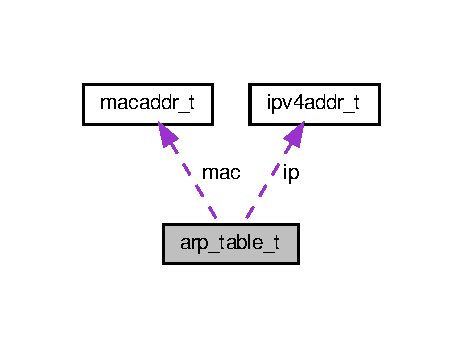
\includegraphics[width=224pt]{structarp__table__t__coll__graph}
\end{center}
\end{figure}
\subsection*{Public Member Functions}
\begin{DoxyCompactItemize}
\item 
\mbox{\Hypertarget{structarp__table__t_a55dbe4612e966b60efa8324e185922dc}\label{structarp__table__t_a55dbe4612e966b60efa8324e185922dc}} 
{\bfseries arp\+\_\+table\+\_\+t} (\hyperlink{macros_8h_a464a07ed2c6d005d677113cc44750a64}{u32t} ip, \hyperlink{macros_8h_a176a4ab0531a048e0693a4520c550193}{u8t} $\ast$mac)
\end{DoxyCompactItemize}
\subsection*{Public Attributes}
\begin{DoxyCompactItemize}
\item 
\mbox{\Hypertarget{structarp__table__t_ac52ee8bea2f590d4bc914c63a308e41e}\label{structarp__table__t_ac52ee8bea2f590d4bc914c63a308e41e}} 
\hyperlink{unionipv4addr__t}{ipv4addr\+\_\+t} {\bfseries ip}
\item 
\mbox{\Hypertarget{structarp__table__t_aa43555ba4be02b3ce8ff25269ef346f0}\label{structarp__table__t_aa43555ba4be02b3ce8ff25269ef346f0}} 
\hyperlink{structmacaddr__t}{macaddr\+\_\+t} {\bfseries mac}
\end{DoxyCompactItemize}


The documentation for this struct was generated from the following file\+:\begin{DoxyCompactItemize}
\item 
arptable.\+h\end{DoxyCompactItemize}

\hypertarget{classArpTable}{}\section{Arp\+Table Class Reference}
\label{classArpTable}\index{Arp\+Table@{Arp\+Table}}
\subsection*{Public Member Functions}
\begin{DoxyCompactItemize}
\item 
\mbox{\Hypertarget{classArpTable_a73005ba2b1e7a304ca8e52fc248fa088}\label{classArpTable_a73005ba2b1e7a304ca8e52fc248fa088}} 
void {\bfseries add\+Record} (\hyperlink{structarp__table__t}{arp\+\_\+table\+\_\+t} entry)
\item 
\mbox{\Hypertarget{classArpTable_a50ff8a76494c612b9d9a3e0959a22319}\label{classArpTable_a50ff8a76494c612b9d9a3e0959a22319}} 
void {\bfseries add\+Record} (\hyperlink{macros_8h_a464a07ed2c6d005d677113cc44750a64}{u32t} ip, \hyperlink{macros_8h_a176a4ab0531a048e0693a4520c550193}{u8t} $\ast$mac)
\item 
\mbox{\Hypertarget{classArpTable_a82253f8a60a10ccf891523af60127107}\label{classArpTable_a82253f8a60a10ccf891523af60127107}} 
void {\bfseries delete\+Record} (\hyperlink{macros_8h_a590a9a8f7df8fabfac6573e21da1922d}{u16t} index)
\item 
\mbox{\Hypertarget{classArpTable_a2caff3ffc36cabf9a3bfc08791fc54c3}\label{classArpTable_a2caff3ffc36cabf9a3bfc08791fc54c3}} 
void {\bfseries delete\+All\+Records} ()
\item 
\mbox{\Hypertarget{classArpTable_a7ccaac9af85787a5d0ac606e7f35d68c}\label{classArpTable_a7ccaac9af85787a5d0ac606e7f35d68c}} 
uint16\+\_\+t {\bfseries get\+Record\+Number} ()
\item 
\mbox{\Hypertarget{classArpTable_a74f045fa2052bfd3d54a61369862e434}\label{classArpTable_a74f045fa2052bfd3d54a61369862e434}} 
\hyperlink{structarp__table__t}{arp\+\_\+table\+\_\+t} {\bfseries get\+Record} (uint16\+\_\+t index)
\item 
\mbox{\Hypertarget{classArpTable_ae546c9a5a0a1711caa273c62840cc04c}\label{classArpTable_ae546c9a5a0a1711caa273c62840cc04c}} 
std\+::vector$<$ \hyperlink{structarp__table__t}{arp\+\_\+table\+\_\+t} $>$ {\bfseries get\+All\+Records} ()
\end{DoxyCompactItemize}
\subsection*{Private Attributes}
\begin{DoxyCompactItemize}
\item 
\mbox{\Hypertarget{classArpTable_a81b942abf2c4e35ca7790939595f59b3}\label{classArpTable_a81b942abf2c4e35ca7790939595f59b3}} 
std\+::vector$<$ \hyperlink{structarp__table__t}{arp\+\_\+table\+\_\+t} $>$ {\bfseries arp\+Table}
\end{DoxyCompactItemize}


The documentation for this class was generated from the following files\+:\begin{DoxyCompactItemize}
\item 
arptable.\+h\item 
arptable.\+cpp\end{DoxyCompactItemize}

\hypertarget{structcompass__t}{}\section{compass\+\_\+t Struct Reference}
\label{structcompass__t}\index{compass\+\_\+t@{compass\+\_\+t}}
\subsection*{Public Attributes}
\begin{DoxyCompactItemize}
\item 
\mbox{\Hypertarget{structcompass__t_aaa5323135e100dea4ba14a5e3d1dc555}\label{structcompass__t_aaa5323135e100dea4ba14a5e3d1dc555}} 
int16\+\_\+t {\bfseries raw\+\_\+x}
\item 
\mbox{\Hypertarget{structcompass__t_a719b0ea8a5f9dda8804bf91b98d8cedf}\label{structcompass__t_a719b0ea8a5f9dda8804bf91b98d8cedf}} 
int16\+\_\+t {\bfseries raw\+\_\+y}
\item 
\mbox{\Hypertarget{structcompass__t_ae7828390c86ad613fd89fa84526dc555}\label{structcompass__t_ae7828390c86ad613fd89fa84526dc555}} 
int16\+\_\+t {\bfseries raw\+\_\+z}
\item 
\mbox{\Hypertarget{structcompass__t_ac4778441994a1a67998c2fd2c3c422f1}\label{structcompass__t_ac4778441994a1a67998c2fd2c3c422f1}} 
float {\bfseries heading\+Degrees}
\end{DoxyCompactItemize}


The documentation for this struct was generated from the following file\+:\begin{DoxyCompactItemize}
\item 
\hyperlink{hmc5883_8h}{hmc5883.\+h}\end{DoxyCompactItemize}

\hypertarget{classDht11}{}\section{Dht11 Class Reference}
\label{classDht11}\index{Dht11@{Dht11}}


Collaboration diagram for Dht11\+:\nopagebreak
\begin{figure}[H]
\begin{center}
\leavevmode
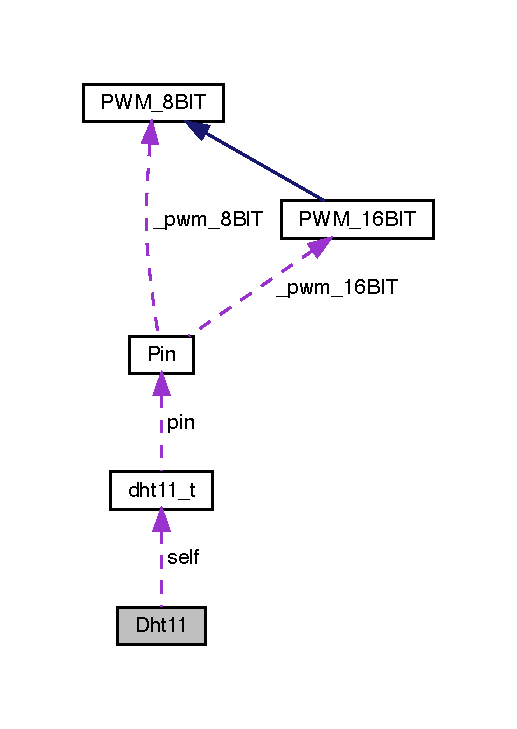
\includegraphics[width=248pt]{classDht11__coll__graph}
\end{center}
\end{figure}
\subsection*{Public Member Functions}
\begin{DoxyCompactItemize}
\item 
\mbox{\Hypertarget{classDht11_a2d28c64f9f68880b48c787fe8be65e82}\label{classDht11_a2d28c64f9f68880b48c787fe8be65e82}} 
{\bfseries Dht11} (\mbox{\hyperlink{classPin}{Pin}} pin)
\item 
\mbox{\Hypertarget{classDht11_aca67610ae8e6e7a2f1df449295944b12}\label{classDht11_aca67610ae8e6e7a2f1df449295944b12}} 
{\bfseries Dht11} (uint8\+\_\+t pin)
\item 
\mbox{\Hypertarget{classDht11_af3721521ff45bfbbe0a6b2ff3801d511}\label{classDht11_af3721521ff45bfbbe0a6b2ff3801d511}} 
{\bfseries Dht11} (\mbox{\hyperlink{structdht11__t}{dht11\+\_\+t}} dht11)
\item 
\mbox{\Hypertarget{classDht11_a0959ad424980bf0386e132b66cbade5c}\label{classDht11_a0959ad424980bf0386e132b66cbade5c}} 
uint8\+\_\+t {\bfseries get\+Temperature} ()
\item 
\mbox{\Hypertarget{classDht11_a7edaa36ffa969932f7522a92d4ebbc21}\label{classDht11_a7edaa36ffa969932f7522a92d4ebbc21}} 
uint8\+\_\+t {\bfseries get\+Humidity} ()
\item 
\mbox{\Hypertarget{classDht11_a2e70616b1c70d2dc6937e38c6cef27de}\label{classDht11_a2e70616b1c70d2dc6937e38c6cef27de}} 
bool {\bfseries start\+Contition} ()
\item 
\mbox{\Hypertarget{classDht11_ad4cb519c841e97b5d1464e1fb66b332f}\label{classDht11_ad4cb519c841e97b5d1464e1fb66b332f}} 
void {\bfseries get\+Data} ()
\item 
\mbox{\Hypertarget{classDht11_aded72886f2b8eed116d027ac47227046}\label{classDht11_aded72886f2b8eed116d027ac47227046}} 
bool {\bfseries check\+Crc} ()
\end{DoxyCompactItemize}
\subsection*{Private Attributes}
\begin{DoxyCompactItemize}
\item 
\mbox{\Hypertarget{classDht11_ad12915cbf961e219ef06dc617389ca51}\label{classDht11_ad12915cbf961e219ef06dc617389ca51}} 
\mbox{\hyperlink{structdht11__t}{dht11\+\_\+t}} {\bfseries self}
\end{DoxyCompactItemize}


The documentation for this class was generated from the following files\+:\begin{DoxyCompactItemize}
\item 
dht11.\+h\item 
dht11.\+cpp\end{DoxyCompactItemize}

\hypertarget{structdht11__t}{}\section{dht11\+\_\+t Struct Reference}
\label{structdht11__t}\index{dht11\_t@{dht11\_t}}


Collaboration diagram for dht11\+\_\+t\+:\nopagebreak
\begin{figure}[H]
\begin{center}
\leavevmode
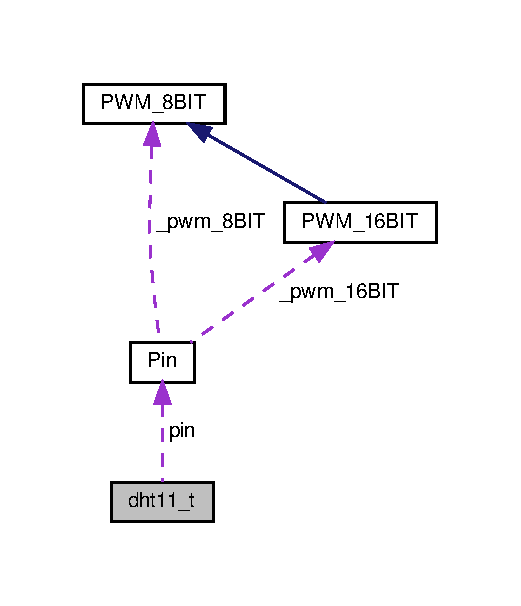
\includegraphics[width=248pt]{structdht11__t__coll__graph}
\end{center}
\end{figure}
\subsection*{Public Attributes}
\begin{DoxyCompactItemize}
\item 
\mbox{\Hypertarget{structdht11__t_af7ba765d61375a8088a63e33b4e91a35}\label{structdht11__t_af7ba765d61375a8088a63e33b4e91a35}} 
\mbox{\hyperlink{classPin}{Pin}} {\bfseries pin}
\item 
\mbox{\Hypertarget{structdht11__t_a981a3577bb83ac4f3f8f566e4eb9976c}\label{structdht11__t_a981a3577bb83ac4f3f8f566e4eb9976c}} 
uint8\+\_\+t {\bfseries humidity}
\item 
\mbox{\Hypertarget{structdht11__t_a3426ca69a0d25e6ff59cf1bb814194d5}\label{structdht11__t_a3426ca69a0d25e6ff59cf1bb814194d5}} 
uint8\+\_\+t {\bfseries humidity\+\_\+float}
\item 
\mbox{\Hypertarget{structdht11__t_acb375c16a957e10e3c316496492263da}\label{structdht11__t_acb375c16a957e10e3c316496492263da}} 
uint8\+\_\+t {\bfseries temperature}
\item 
\mbox{\Hypertarget{structdht11__t_aebb3d3b42b5c014880980fc77af3f7b6}\label{structdht11__t_aebb3d3b42b5c014880980fc77af3f7b6}} 
uint8\+\_\+t {\bfseries temperature\+\_\+float}
\item 
\mbox{\Hypertarget{structdht11__t_a51b07566b9cee55f9c9f473d4bda96d1}\label{structdht11__t_a51b07566b9cee55f9c9f473d4bda96d1}} 
uint8\+\_\+t {\bfseries crc}
\end{DoxyCompactItemize}


The documentation for this struct was generated from the following file\+:\begin{DoxyCompactItemize}
\item 
dht11.\+h\end{DoxyCompactItemize}

\hypertarget{classEnc28j60}{}\section{Enc28j60 Class Reference}
\label{classEnc28j60}\index{Enc28j60@{Enc28j60}}


Collaboration diagram for Enc28j60\+:\nopagebreak
\begin{figure}[H]
\begin{center}
\leavevmode
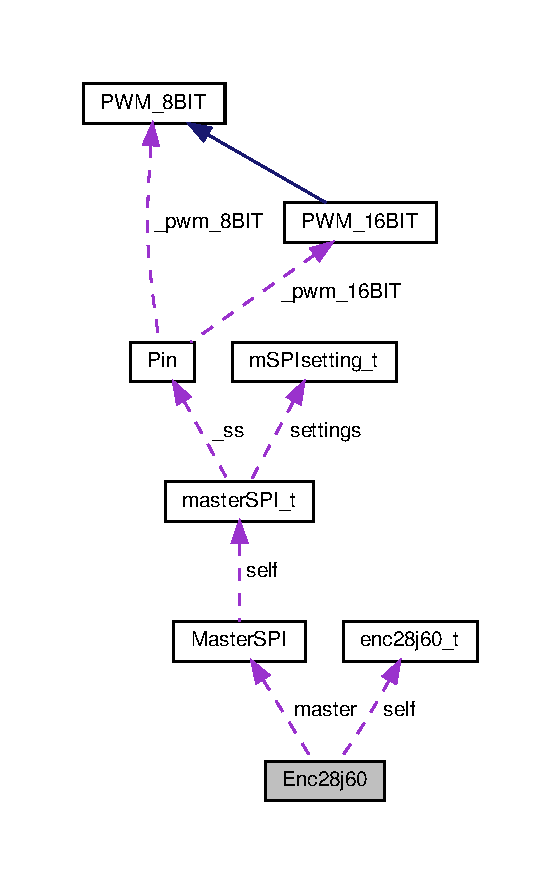
\includegraphics[width=268pt]{classEnc28j60__coll__graph}
\end{center}
\end{figure}
\subsection*{Public Member Functions}
\begin{DoxyCompactItemize}
\item 
\mbox{\Hypertarget{classEnc28j60_a02091be5ccc917e0e2faaa7053e9340d}\label{classEnc28j60_a02091be5ccc917e0e2faaa7053e9340d}} 
bool {\bfseries init} (std\+::string ip, std\+::vector$<$ uint8\+\_\+t $>$ \&mac)
\item 
\mbox{\Hypertarget{classEnc28j60_a52b9b6f5b16f09bf6734cbd92283fa01}\label{classEnc28j60_a52b9b6f5b16f09bf6734cbd92283fa01}} 
void {\bfseries set\+S\+PI} (uint8\+\_\+t miso, uint8\+\_\+t mosi, uint8\+\_\+t sck, uint8\+\_\+t ss)
\item 
\mbox{\Hypertarget{classEnc28j60_aa35d466c70b46fe8a8c23c688fe12bfa}\label{classEnc28j60_aa35d466c70b46fe8a8c23c688fe12bfa}} 
std\+::vector$<$ uint8\+\_\+t $>$ {\bfseries get\+M\+AC} ()
\item 
\mbox{\Hypertarget{classEnc28j60_ad26a59006c5dc25efe10e7787e10ad8d}\label{classEnc28j60_ad26a59006c5dc25efe10e7787e10ad8d}} 
void {\bfseries set\+M\+AC} (std\+::vector$<$ uint8\+\_\+t $>$ \&mac)
\item 
\mbox{\Hypertarget{classEnc28j60_a6725c414929ca567d39c30ddd2cebbc3}\label{classEnc28j60_a6725c414929ca567d39c30ddd2cebbc3}} 
void {\bfseries send} ()
\item 
\mbox{\Hypertarget{classEnc28j60_a3186dc79ca3d83c0f68f7d8479a2df4a}\label{classEnc28j60_a3186dc79ca3d83c0f68f7d8479a2df4a}} 
uint8\+\_\+t {\bfseries \+\_\+get\+Revision\+ID} ()
\end{DoxyCompactItemize}
\subsection*{Private Member Functions}
\begin{DoxyCompactItemize}
\item 
\mbox{\Hypertarget{classEnc28j60_a8aa52f4f9150cfd8975c01c388952be3}\label{classEnc28j60_a8aa52f4f9150cfd8975c01c388952be3}} 
uint8\+\_\+t {\bfseries read\+Reg} (uint8\+\_\+t reg)
\item 
\mbox{\Hypertarget{classEnc28j60_a44f843303ed9e671e867910c337d4421}\label{classEnc28j60_a44f843303ed9e671e867910c337d4421}} 
void {\bfseries write\+Reg} (uint8\+\_\+t reg, uint8\+\_\+t data)
\item 
\mbox{\Hypertarget{classEnc28j60_a52901d3be0ae0b8ad202927a2e7e3d0f}\label{classEnc28j60_a52901d3be0ae0b8ad202927a2e7e3d0f}} 
void {\bfseries read\+Buff\+Memory} (std\+::vector$<$ uint8\+\_\+t $>$ \&buff, size\+\_\+t size)
\item 
\mbox{\Hypertarget{classEnc28j60_ac242c72302b61d6d4b81508935665c8c}\label{classEnc28j60_ac242c72302b61d6d4b81508935665c8c}} 
void {\bfseries write\+Buff\+Memory} (std\+::vector$<$ uint8\+\_\+t $>$ \&buff)
\item 
\mbox{\Hypertarget{classEnc28j60_ac5853b6da39441aa8370bd3e809a3fd8}\label{classEnc28j60_ac5853b6da39441aa8370bd3e809a3fd8}} 
void {\bfseries bit\+Field\+Set} (uint8\+\_\+t reg, uint8\+\_\+t data)
\item 
\mbox{\Hypertarget{classEnc28j60_a60cd171ca97f496cbf51350c743e8247}\label{classEnc28j60_a60cd171ca97f496cbf51350c743e8247}} 
void {\bfseries bit\+Field\+Clear} (uint8\+\_\+t reg, uint8\+\_\+t data)
\item 
\mbox{\Hypertarget{classEnc28j60_a823d4bd466e9fd160c8730141c8e2e83}\label{classEnc28j60_a823d4bd466e9fd160c8730141c8e2e83}} 
void {\bfseries write\+OP} (\mbox{\hyperlink{structENC28J60__ISA}{E\+N\+C28\+J60\+\_\+\+I\+SA}} cmd)
\item 
\mbox{\Hypertarget{classEnc28j60_a7be0cb9c172c45453783009636548d09}\label{classEnc28j60_a7be0cb9c172c45453783009636548d09}} 
uint8\+\_\+t {\bfseries read\+OP} (\mbox{\hyperlink{structENC28J60__ISA}{E\+N\+C28\+J60\+\_\+\+I\+SA}} cmd)
\item 
\mbox{\Hypertarget{classEnc28j60_a3d0223a215213be14cccf8a6eb4c65e6}\label{classEnc28j60_a3d0223a215213be14cccf8a6eb4c65e6}} 
void {\bfseries select\+Bank} (uint8\+\_\+t bank)
\item 
\mbox{\Hypertarget{classEnc28j60_a1293d524f38225318c67bec2856c2cf3}\label{classEnc28j60_a1293d524f38225318c67bec2856c2cf3}} 
void {\bfseries reset} ()
\item 
\mbox{\Hypertarget{classEnc28j60_a7c5ee483693710bc8c973413e52dc5b9}\label{classEnc28j60_a7c5ee483693710bc8c973413e52dc5b9}} 
void {\bfseries init\+Receive\+Buff} ()
\item 
\mbox{\Hypertarget{classEnc28j60_aea901773a26edf7e13a0aa249ef354d2}\label{classEnc28j60_aea901773a26edf7e13a0aa249ef354d2}} 
void {\bfseries init\+Transmit\+Buff} ()
\item 
\mbox{\Hypertarget{classEnc28j60_a801b7b936e24295f75a51ccce398c61c}\label{classEnc28j60_a801b7b936e24295f75a51ccce398c61c}} 
void {\bfseries enable\+Mac\+Receive} ()
\item 
\mbox{\Hypertarget{classEnc28j60_a257b08a023955ade7d226e3c9a199780}\label{classEnc28j60_a257b08a023955ade7d226e3c9a199780}} 
void {\bfseries enable\+Auto\+Pad\+Crc} ()
\item 
\mbox{\Hypertarget{classEnc28j60_af4f9dbaf022b144ffea766c97630c902}\label{classEnc28j60_af4f9dbaf022b144ffea766c97630c902}} 
void {\bfseries set\+Max\+Packet\+Size} ()
\end{DoxyCompactItemize}
\subsection*{Private Attributes}
\begin{DoxyCompactItemize}
\item 
\mbox{\Hypertarget{classEnc28j60_a397a8e8f650313321fad2ad320e52b9e}\label{classEnc28j60_a397a8e8f650313321fad2ad320e52b9e}} 
\mbox{\hyperlink{structenc28j60__t}{enc28j60\+\_\+t}} {\bfseries self}
\item 
\mbox{\Hypertarget{classEnc28j60_add18edc29b10e89bacc3e83ecd2b51fb}\label{classEnc28j60_add18edc29b10e89bacc3e83ecd2b51fb}} 
\mbox{\hyperlink{classMasterSPI}{Master\+S\+PI}} $\ast$ {\bfseries master}
\end{DoxyCompactItemize}


The documentation for this class was generated from the following files\+:\begin{DoxyCompactItemize}
\item 
enc28j60.\+h\item 
enc28j60.\+cpp\end{DoxyCompactItemize}

\hypertarget{structENC28J60__ISA}{}\section{E\+N\+C28\+J60\+\_\+\+I\+SA Struct Reference}
\label{structENC28J60__ISA}\index{ENC28J60\_ISA@{ENC28J60\_ISA}}
\subsection*{Public Member Functions}
\begin{DoxyCompactItemize}
\item 
\mbox{\Hypertarget{structENC28J60__ISA_a79c2254ac740145cea5d92bd14e35a0c}\label{structENC28J60__ISA_a79c2254ac740145cea5d92bd14e35a0c}} 
{\bfseries E\+N\+C28\+J60\+\_\+\+I\+SA} (uint16\+\_\+t packet=0)
\end{DoxyCompactItemize}
\subsection*{Public Attributes}
\begin{DoxyCompactItemize}
\item 
\mbox{\Hypertarget{structENC28J60__ISA_a10bc49b8ef6d4f91a6f2302758c1fb71}\label{structENC28J60__ISA_a10bc49b8ef6d4f91a6f2302758c1fb71}} 
\begin{tabbing}
xx\=xx\=xx\=xx\=xx\=xx\=xx\=xx\=xx\=\kill
union \{\\
\>struct \{\\
\>\>union \{\\
\>\>\>struct \{\\
\>\>\>\>uint8\_t {\bfseries opcode}:3\\
\>\>\>\>uint8\_t {\bfseries argument}:5\\
\>\>\>\} {\bfseries fields}\\
\>\>\>uint8\_t {\bfseries data}\\
\>\>\} {\bfseries byte0}\\
\>\>uint8\_t {\bfseries payload}\\
\>\} {\bfseries cmd}\\
\>uint16\_t {\bfseries packet}\\
\}; \\

\end{tabbing}\end{DoxyCompactItemize}


The documentation for this struct was generated from the following file\+:\begin{DoxyCompactItemize}
\item 
enc28j60.\+h\end{DoxyCompactItemize}

\hypertarget{structenc28j60__t}{}\section{enc28j60\+\_\+t Struct Reference}
\label{structenc28j60__t}\index{enc28j60\_t@{enc28j60\_t}}
\subsection*{Public Attributes}
\begin{DoxyCompactItemize}
\item 
\mbox{\Hypertarget{structenc28j60__t_a657dad5c4c332641d1b43f4bfb767242}\label{structenc28j60__t_a657dad5c4c332641d1b43f4bfb767242}} 
std\+::vector$<$ uint8\+\_\+t $>$ {\bfseries M\+A\+C\+Address} \mbox{[}6\mbox{]}
\item 
\mbox{\Hypertarget{structenc28j60__t_ada7729afae8752ce121d1c113823dbab}\label{structenc28j60__t_ada7729afae8752ce121d1c113823dbab}} 
uint8\+\_\+t {\bfseries revision\+ID}
\item 
\mbox{\Hypertarget{structenc28j60__t_a606c78d2b4ecbad4bf211c8fd0f5b8d0}\label{structenc28j60__t_a606c78d2b4ecbad4bf211c8fd0f5b8d0}} 
bool {\bfseries full\+Duplex}
\item 
\mbox{\Hypertarget{structenc28j60__t_aa1da4572ba169749318a0ac87c4df06a}\label{structenc28j60__t_aa1da4572ba169749318a0ac87c4df06a}} 
uint8\+\_\+t {\bfseries current\+Bank}
\item 
\mbox{\Hypertarget{structenc28j60__t_a70a59370e15b65d068cfd2b7c401aa97}\label{structenc28j60__t_a70a59370e15b65d068cfd2b7c401aa97}} 
uint16\+\_\+t {\bfseries next\+Packet\+Ptr}
\end{DoxyCompactItemize}


The documentation for this struct was generated from the following file\+:\begin{DoxyCompactItemize}
\item 
enc28j60.\+h\end{DoxyCompactItemize}

\hypertarget{structeth__frame__t}{}\section{eth\+\_\+frame\+\_\+t Struct Reference}
\label{structeth__frame__t}\index{eth\+\_\+frame\+\_\+t@{eth\+\_\+frame\+\_\+t}}


Collaboration diagram for eth\+\_\+frame\+\_\+t\+:\nopagebreak
\begin{figure}[H]
\begin{center}
\leavevmode
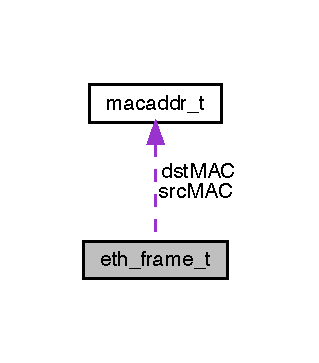
\includegraphics[width=153pt]{structeth__frame__t__coll__graph}
\end{center}
\end{figure}
\subsection*{Public Member Functions}
\begin{DoxyCompactItemize}
\item 
\mbox{\Hypertarget{structeth__frame__t_a8617affa4463b4e4b29484ddc6704ae1}\label{structeth__frame__t_a8617affa4463b4e4b29484ddc6704ae1}} 
{\bfseries eth\+\_\+frame\+\_\+t} (\hyperlink{structmacaddr__t}{macaddr\+\_\+t} dst\+M\+AC=\hyperlink{structmacaddr__t}{macaddr\+\_\+t}(), \hyperlink{structmacaddr__t}{macaddr\+\_\+t} src\+M\+AC=\hyperlink{structmacaddr__t}{macaddr\+\_\+t}(), \hyperlink{macros_8h_a590a9a8f7df8fabfac6573e21da1922d}{u16t} ether\+Type=0, \hyperlink{macros_8h_a464a07ed2c6d005d677113cc44750a64}{u32t} crc=0, \hyperlink{macros_8h_a176a4ab0531a048e0693a4520c550193}{u8t} $\ast$interpacket\+\_\+gap=nullptr)
\end{DoxyCompactItemize}
\subsection*{Public Attributes}
\begin{DoxyCompactItemize}
\item 
\mbox{\Hypertarget{structeth__frame__t_a7e917da155e1a71584d77ba116c51537}\label{structeth__frame__t_a7e917da155e1a71584d77ba116c51537}} 
\hyperlink{macros_8h_a176a4ab0531a048e0693a4520c550193}{u8t} {\bfseries preamble} \mbox{[}7\mbox{]} = \{0x55, 0x55, 0x55, 0x55, 0x55, 0x55, 0x55\}
\item 
\mbox{\Hypertarget{structeth__frame__t_a2373b35ac05da6d436fa1369a9868417}\label{structeth__frame__t_a2373b35ac05da6d436fa1369a9868417}} 
\hyperlink{macros_8h_a176a4ab0531a048e0693a4520c550193}{u8t} {\bfseries S\+FD} = 0x\+D5
\item 
\mbox{\Hypertarget{structeth__frame__t_ac8ac769f22710edece8c5de6f206b793}\label{structeth__frame__t_ac8ac769f22710edece8c5de6f206b793}} 
\hyperlink{structmacaddr__t}{macaddr\+\_\+t} {\bfseries dst\+M\+AC}
\item 
\mbox{\Hypertarget{structeth__frame__t_a23bd734d1f17859fca7aa01cf036e21d}\label{structeth__frame__t_a23bd734d1f17859fca7aa01cf036e21d}} 
\hyperlink{structmacaddr__t}{macaddr\+\_\+t} {\bfseries src\+M\+AC}
\item 
\mbox{\Hypertarget{structeth__frame__t_a955b35cc93d08eab023f0fa1383a6107}\label{structeth__frame__t_a955b35cc93d08eab023f0fa1383a6107}} 
\hyperlink{macros_8h_a590a9a8f7df8fabfac6573e21da1922d}{u16t} {\bfseries ether\+Type}
\item 
\mbox{\Hypertarget{structeth__frame__t_aa4b072edd94e393936b674c077dcf001}\label{structeth__frame__t_aa4b072edd94e393936b674c077dcf001}} 
std\+::vector$<$ \hyperlink{macros_8h_a176a4ab0531a048e0693a4520c550193}{u8t} $>$ {\bfseries payload}
\item 
\mbox{\Hypertarget{structeth__frame__t_ab479ce46f2f16015beb4f05eccae7b52}\label{structeth__frame__t_ab479ce46f2f16015beb4f05eccae7b52}} 
\hyperlink{macros_8h_a464a07ed2c6d005d677113cc44750a64}{u32t} {\bfseries crc}
\item 
\mbox{\Hypertarget{structeth__frame__t_aa64d327330c12dd5675c9b3ea5b717db}\label{structeth__frame__t_aa64d327330c12dd5675c9b3ea5b717db}} 
\hyperlink{macros_8h_a176a4ab0531a048e0693a4520c550193}{u8t} {\bfseries interpacket\+\_\+gap} \mbox{[}12\mbox{]}
\end{DoxyCompactItemize}


The documentation for this struct was generated from the following file\+:\begin{DoxyCompactItemize}
\item 
inet\+\_\+global.\+h\end{DoxyCompactItemize}

\hypertarget{structeth__vlan__frame__t}{}\section{eth\+\_\+vlan\+\_\+frame\+\_\+t Struct Reference}
\label{structeth__vlan__frame__t}\index{eth\+\_\+vlan\+\_\+frame\+\_\+t@{eth\+\_\+vlan\+\_\+frame\+\_\+t}}


Collaboration diagram for eth\+\_\+vlan\+\_\+frame\+\_\+t\+:\nopagebreak
\begin{figure}[H]
\begin{center}
\leavevmode
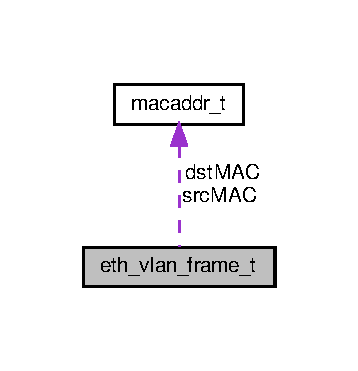
\includegraphics[width=172pt]{structeth__vlan__frame__t__coll__graph}
\end{center}
\end{figure}
\subsection*{Public Member Functions}
\begin{DoxyCompactItemize}
\item 
\mbox{\Hypertarget{structeth__vlan__frame__t_afd8ff79bdc0fd97dd158d1b0e6842363}\label{structeth__vlan__frame__t_afd8ff79bdc0fd97dd158d1b0e6842363}} 
{\bfseries eth\+\_\+vlan\+\_\+frame\+\_\+t} (\hyperlink{structmacaddr__t}{macaddr\+\_\+t} dst\+M\+AC=\hyperlink{structmacaddr__t}{macaddr\+\_\+t}(), \hyperlink{structmacaddr__t}{macaddr\+\_\+t} src\+M\+AC=\hyperlink{structmacaddr__t}{macaddr\+\_\+t}(), u32t vlan\+Tag=0, u16t ether\+Type=0, u32t crc=0, u8t $\ast$interpacket\+\_\+gap=nullptr)
\end{DoxyCompactItemize}
\subsection*{Public Attributes}
\begin{DoxyCompactItemize}
\item 
\mbox{\Hypertarget{structeth__vlan__frame__t_a78999322e3f11cb4c7e64f63671c9200}\label{structeth__vlan__frame__t_a78999322e3f11cb4c7e64f63671c9200}} 
u8t {\bfseries preamble} \mbox{[}7\mbox{]} = \{0x55, 0x55, 0x55, 0x55, 0x55, 0x55, 0x55\}
\item 
\mbox{\Hypertarget{structeth__vlan__frame__t_a69b29b6322d0d6d73939bff432538d06}\label{structeth__vlan__frame__t_a69b29b6322d0d6d73939bff432538d06}} 
u8t {\bfseries S\+FD} = 0x\+D5
\item 
\mbox{\Hypertarget{structeth__vlan__frame__t_af65384a13f1fbccc547ffcd5bd1914c1}\label{structeth__vlan__frame__t_af65384a13f1fbccc547ffcd5bd1914c1}} 
\hyperlink{structmacaddr__t}{macaddr\+\_\+t} {\bfseries dst\+M\+AC}
\item 
\mbox{\Hypertarget{structeth__vlan__frame__t_ae08beab62fa2486d9e06746fc62d5ae0}\label{structeth__vlan__frame__t_ae08beab62fa2486d9e06746fc62d5ae0}} 
\hyperlink{structmacaddr__t}{macaddr\+\_\+t} {\bfseries src\+M\+AC}
\item 
\mbox{\Hypertarget{structeth__vlan__frame__t_a2170006324fff8cb5f96172a340ef852}\label{structeth__vlan__frame__t_a2170006324fff8cb5f96172a340ef852}} 
u32t {\bfseries vlan\+Tag}
\item 
\mbox{\Hypertarget{structeth__vlan__frame__t_ab1a9bcb061996b0a8a384c89ae7477dc}\label{structeth__vlan__frame__t_ab1a9bcb061996b0a8a384c89ae7477dc}} 
u16t {\bfseries ether\+Type}
\item 
\mbox{\Hypertarget{structeth__vlan__frame__t_a3724d5d625e71ba2008fa1d058b1be76}\label{structeth__vlan__frame__t_a3724d5d625e71ba2008fa1d058b1be76}} 
std\+::vector$<$ uint8\+\_\+t $>$ {\bfseries payload}
\item 
\mbox{\Hypertarget{structeth__vlan__frame__t_a99ce30cc2b1b0c61306f056e71aa497d}\label{structeth__vlan__frame__t_a99ce30cc2b1b0c61306f056e71aa497d}} 
u32t {\bfseries crc}
\item 
\mbox{\Hypertarget{structeth__vlan__frame__t_aa68bb1e435d49b46770315990b3e2021}\label{structeth__vlan__frame__t_aa68bb1e435d49b46770315990b3e2021}} 
u8t {\bfseries interpacket\+\_\+gap} \mbox{[}12\mbox{]}
\end{DoxyCompactItemize}


The documentation for this struct was generated from the following file\+:\begin{DoxyCompactItemize}
\item 
inet\+\_\+global.\+h\end{DoxyCompactItemize}

\hypertarget{classEthernet}{}\section{Ethernet Class Reference}
\label{classEthernet}\index{Ethernet@{Ethernet}}


Collaboration diagram for Ethernet\+:\nopagebreak
\begin{figure}[H]
\begin{center}
\leavevmode
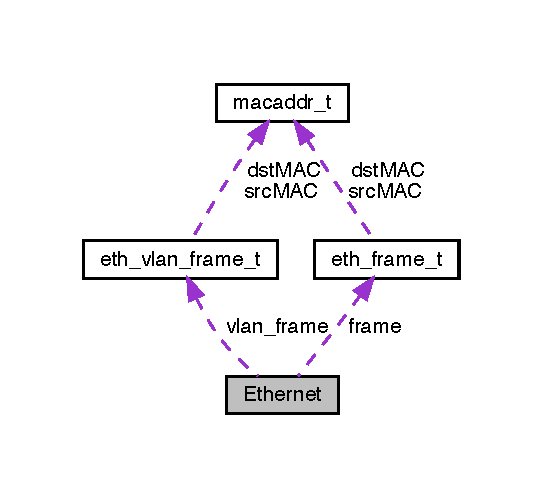
\includegraphics[width=258pt]{classEthernet__coll__graph}
\end{center}
\end{figure}
\subsection*{Public Member Functions}
\begin{DoxyCompactItemize}
\item 
\mbox{\Hypertarget{classEthernet_a0ee0a7b0720489214113bde0fb14fd12}\label{classEthernet_a0ee0a7b0720489214113bde0fb14fd12}} 
bool {\bfseries encapsulate} (std\+::vector$<$ u8t $>$ \&payload)
\item 
\mbox{\Hypertarget{classEthernet_a6a3304c3cd5c3b79049d24fcc2854f48}\label{classEthernet_a6a3304c3cd5c3b79049d24fcc2854f48}} 
void {\bfseries decapsulate} (std\+::vector$<$ u8t $>$ \&data)
\end{DoxyCompactItemize}
\subsection*{Private Attributes}
\begin{DoxyCompactItemize}
\item 
\mbox{\Hypertarget{classEthernet_a9d4e1ec352eb5209d5675592aebfdd85}\label{classEthernet_a9d4e1ec352eb5209d5675592aebfdd85}} 
\hyperlink{structeth__frame__t}{eth\+\_\+frame\+\_\+t} {\bfseries frame}
\item 
\mbox{\Hypertarget{classEthernet_ad6f419f6b4c1050af2d4b974186d862e}\label{classEthernet_ad6f419f6b4c1050af2d4b974186d862e}} 
\hyperlink{structeth__vlan__frame__t}{eth\+\_\+vlan\+\_\+frame\+\_\+t} {\bfseries vlan\+\_\+frame}
\end{DoxyCompactItemize}


The documentation for this class was generated from the following files\+:\begin{DoxyCompactItemize}
\item 
ethernet.\+h\item 
ethernet.\+cpp\end{DoxyCompactItemize}

\hypertarget{classHmc5883}{}\section{Hmc5883 Class Reference}
\label{classHmc5883}\index{Hmc5883@{Hmc5883}}


Collaboration diagram for Hmc5883\+:\nopagebreak
\begin{figure}[H]
\begin{center}
\leavevmode
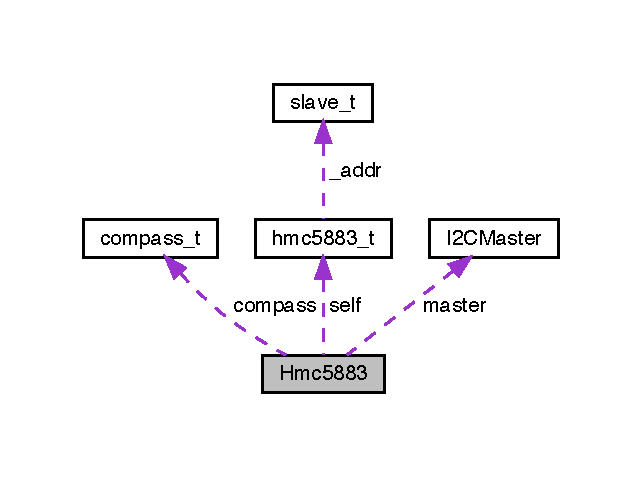
\includegraphics[width=308pt]{classHmc5883__coll__graph}
\end{center}
\end{figure}
\subsection*{Public Member Functions}
\begin{DoxyCompactItemize}
\item 
\mbox{\Hypertarget{classHmc5883_ac524eb35511c0cc1af4fde7c25ce6bc8}\label{classHmc5883_ac524eb35511c0cc1af4fde7c25ce6bc8}} 
{\bfseries Hmc5883} (uint8\+\_\+t write\+Addr=0x3c, uint8\+\_\+t read\+Addr=0x3d)
\item 
\mbox{\Hypertarget{classHmc5883_ab21eb9fe07af129ca5f838b568183d7b}\label{classHmc5883_ab21eb9fe07af129ca5f838b568183d7b}} 
void {\bfseries init} ()
\item 
\mbox{\Hypertarget{classHmc5883_a11189f87dac5ff48217551fc76d3c93b}\label{classHmc5883_a11189f87dac5ff48217551fc76d3c93b}} 
\mbox{\hyperlink{structcompass__t}{compass\+\_\+t}} {\bfseries get\+Data} ()
\item 
\mbox{\Hypertarget{classHmc5883_a69dbf7355977a9b33ca7910d8f716095}\label{classHmc5883_a69dbf7355977a9b33ca7910d8f716095}} 
void {\bfseries set\+Sample} (S\+A\+M\+P\+L\+E\+\_\+\+M\+E\+A\+S\+U\+RE sample)
\item 
\mbox{\Hypertarget{classHmc5883_aa2592ac2bfc5a4e98c13ed278fa8f414}\label{classHmc5883_aa2592ac2bfc5a4e98c13ed278fa8f414}} 
S\+A\+M\+P\+L\+E\+\_\+\+M\+E\+A\+S\+U\+RE {\bfseries get\+Sample} ()
\item 
\mbox{\Hypertarget{classHmc5883_af850118d4a20b7622aa796d8dbca5662}\label{classHmc5883_af850118d4a20b7622aa796d8dbca5662}} 
void {\bfseries set\+Out\+Rate} ()
\item 
\mbox{\Hypertarget{classHmc5883_a692ad42338c883012ec5b11347e1bfd8}\label{classHmc5883_a692ad42338c883012ec5b11347e1bfd8}} 
O\+U\+T\+P\+U\+T\+\_\+\+R\+A\+TE {\bfseries get\+Out\+Rate} ()
\item 
\mbox{\Hypertarget{classHmc5883_a106b6982d67ef293f8f4d7f5dd3bff46}\label{classHmc5883_a106b6982d67ef293f8f4d7f5dd3bff46}} 
void {\bfseries set\+Gain} ()
\item 
\mbox{\Hypertarget{classHmc5883_a9a2dc9a1b419a096ebf7aacb1a2e0ef3}\label{classHmc5883_a9a2dc9a1b419a096ebf7aacb1a2e0ef3}} 
G\+A\+IN {\bfseries get\+Gain} ()
\item 
\mbox{\Hypertarget{classHmc5883_a4f244d6aa1a8f37f7ca77bc4d456ba85}\label{classHmc5883_a4f244d6aa1a8f37f7ca77bc4d456ba85}} 
void {\bfseries set\+Op\+Mode} ()
\item 
\mbox{\Hypertarget{classHmc5883_a522657db88177c0cca2b64741f796e7d}\label{classHmc5883_a522657db88177c0cca2b64741f796e7d}} 
O\+P\+\_\+\+M\+O\+DE {\bfseries get\+Op\+Mode} ()
\item 
\mbox{\Hypertarget{classHmc5883_a3264769daed5ee49c9ce3011b07abc3d}\label{classHmc5883_a3264769daed5ee49c9ce3011b07abc3d}} 
void {\bfseries set\+Measure\+Mode} ()
\item 
\mbox{\Hypertarget{classHmc5883_ac514cf477af1b8f325bc9d3d7837d5ff}\label{classHmc5883_ac514cf477af1b8f325bc9d3d7837d5ff}} 
M\+E\+A\+S\+U\+R\+E\+\_\+\+M\+O\+DE {\bfseries get\+Measure\+Mode} ()
\end{DoxyCompactItemize}
\subsection*{Private Member Functions}
\begin{DoxyCompactItemize}
\item 
\mbox{\Hypertarget{classHmc5883_ad4af7af089cc97b70cd75f705773e509}\label{classHmc5883_ad4af7af089cc97b70cd75f705773e509}} 
void {\bfseries get\+Heading} ()
\end{DoxyCompactItemize}
\subsection*{Private Attributes}
\begin{DoxyCompactItemize}
\item 
\mbox{\Hypertarget{classHmc5883_a7864e224789881243d69cefce89d7918}\label{classHmc5883_a7864e224789881243d69cefce89d7918}} 
\mbox{\hyperlink{structhmc5883__t}{hmc5883\+\_\+t}} {\bfseries self}
\item 
\mbox{\Hypertarget{classHmc5883_a8c46d4fe172002c5020423939d2e98d1}\label{classHmc5883_a8c46d4fe172002c5020423939d2e98d1}} 
\mbox{\hyperlink{classI2CMaster}{I2\+C\+Master}} {\bfseries master}
\item 
\mbox{\Hypertarget{classHmc5883_a3db3c0edeb0859b84b4530f935bc75b1}\label{classHmc5883_a3db3c0edeb0859b84b4530f935bc75b1}} 
\mbox{\hyperlink{structcompass__t}{compass\+\_\+t}} {\bfseries compass}
\end{DoxyCompactItemize}


The documentation for this class was generated from the following files\+:\begin{DoxyCompactItemize}
\item 
hmc5883.\+h\item 
hmc5883.\+cpp\end{DoxyCompactItemize}

\hypertarget{structhmc5883__t}{}\section{hmc5883\+\_\+t Struct Reference}
\label{structhmc5883__t}\index{hmc5883\+\_\+t@{hmc5883\+\_\+t}}


Collaboration diagram for hmc5883\+\_\+t\+:\nopagebreak
\begin{figure}[H]
\begin{center}
\leavevmode
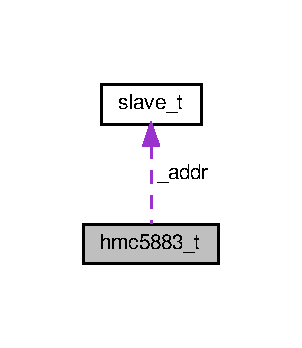
\includegraphics[width=145pt]{structhmc5883__t__coll__graph}
\end{center}
\end{figure}
\subsection*{Public Member Functions}
\begin{DoxyCompactItemize}
\item 
\mbox{\Hypertarget{structhmc5883__t_ada60b7eb8c551a11403cac80c69ad222}\label{structhmc5883__t_ada60b7eb8c551a11403cac80c69ad222}} 
{\bfseries hmc5883\+\_\+t} (\hyperlink{structslave__t}{slave\+\_\+t} addr=0, S\+A\+M\+P\+L\+E\+\_\+\+M\+E\+A\+S\+U\+RE sample=A\+V\+G\+\_\+1, O\+U\+T\+P\+U\+T\+\_\+\+R\+A\+TE out\+Rate=R\+A\+T\+E\+\_\+15\+Hz, G\+A\+IN gain=R\+A\+N\+G\+E\+\_\+1\+\_\+30\+Ga, O\+P\+\_\+\+M\+O\+DE op\+Mode=C\+O\+N\+T\+I\+N\+U\+O\+U\+S\+\_\+\+M\+O\+DE, M\+E\+A\+S\+U\+R\+E\+\_\+\+M\+O\+DE measure\+Mode=D\+E\+F\+\_\+\+B\+I\+AS)
\end{DoxyCompactItemize}
\subsection*{Public Attributes}
\begin{DoxyCompactItemize}
\item 
\mbox{\Hypertarget{structhmc5883__t_a78fcab12d61314413e2000223c8acc9b}\label{structhmc5883__t_a78fcab12d61314413e2000223c8acc9b}} 
\hyperlink{structslave__t}{slave\+\_\+t} {\bfseries \+\_\+addr}
\item 
\mbox{\Hypertarget{structhmc5883__t_a5d6bda3e7c498f9338bf60d4eb0676f1}\label{structhmc5883__t_a5d6bda3e7c498f9338bf60d4eb0676f1}} 
S\+A\+M\+P\+L\+E\+\_\+\+M\+E\+A\+S\+U\+RE {\bfseries \+\_\+sample}
\item 
\mbox{\Hypertarget{structhmc5883__t_abdd992bb7c065497ba272dff4bd5b5fc}\label{structhmc5883__t_abdd992bb7c065497ba272dff4bd5b5fc}} 
O\+U\+T\+P\+U\+T\+\_\+\+R\+A\+TE {\bfseries \+\_\+out\+Rate}
\item 
\mbox{\Hypertarget{structhmc5883__t_adafec64b6dd1f3fab546d3af997ccd0e}\label{structhmc5883__t_adafec64b6dd1f3fab546d3af997ccd0e}} 
G\+A\+IN {\bfseries \+\_\+gain}
\item 
\mbox{\Hypertarget{structhmc5883__t_ae5ae94558f6f65fc5bfda7c3cd23c0da}\label{structhmc5883__t_ae5ae94558f6f65fc5bfda7c3cd23c0da}} 
O\+P\+\_\+\+M\+O\+DE {\bfseries \+\_\+op\+Mode}
\item 
\mbox{\Hypertarget{structhmc5883__t_ab81da8b66db5c81e2d5104b018cca68d}\label{structhmc5883__t_ab81da8b66db5c81e2d5104b018cca68d}} 
M\+E\+A\+S\+U\+R\+E\+\_\+\+M\+O\+DE {\bfseries \+\_\+measure\+Mode}
\end{DoxyCompactItemize}


The documentation for this struct was generated from the following file\+:\begin{DoxyCompactItemize}
\item 
\hyperlink{hmc5883_8h}{hmc5883.\+h}\end{DoxyCompactItemize}

\hypertarget{structHW__INT__PIN}{}\section{H\+W\+\_\+\+I\+N\+T\+\_\+\+P\+IN Struct Reference}
\label{structHW__INT__PIN}\index{H\+W\+\_\+\+I\+N\+T\+\_\+\+P\+IN@{H\+W\+\_\+\+I\+N\+T\+\_\+\+P\+IN}}


The \hyperlink{structHW__INT__PIN}{H\+W\+\_\+\+I\+N\+T\+\_\+\+P\+IN} struct.  




{\ttfamily \#include $<$interrupt.\+h$>$}

\subsection*{Public Attributes}
\begin{DoxyCompactItemize}
\item 
\mbox{\Hypertarget{structHW__INT__PIN_a69d9ddba3cc41c69082271c88e3b9620}\label{structHW__INT__PIN_a69d9ddba3cc41c69082271c88e3b9620}} 
uint8\+\_\+t {\bfseries mapped\+Pin}
\item 
\mbox{\Hypertarget{structHW__INT__PIN_a9f324c3632281053376de195c8a4401a}\label{structHW__INT__PIN_a9f324c3632281053376de195c8a4401a}} 
uint8\+\_\+t {\bfseries E\+I\+C\+Rx}
\item 
\mbox{\Hypertarget{structHW__INT__PIN_a553e9442be5f738b892a8d065b274313}\label{structHW__INT__PIN_a553e9442be5f738b892a8d065b274313}} 
volatile \hyperlink{interrupt_8h_af3e04027ddcd2e23670a55888d788d13}{int\+\_\+cb\+\_\+t} $\ast$$\ast$ {\bfseries interrupt\+Callback}
\item 
\mbox{\Hypertarget{structHW__INT__PIN_aeca115b23cb1b3a6130444eb6de309b6}\label{structHW__INT__PIN_aeca115b23cb1b3a6130444eb6de309b6}} 
\hyperlink{interrupt_8h_affe9baf0034f4cbb8aec6ed2c42b1676}{I\+N\+T\+\_\+\+E\+D\+GE} $\ast$ {\bfseries px\+\_\+edge}
\item 
\mbox{\Hypertarget{structHW__INT__PIN_ad2a69e2c92f937cfde12c0eaca5d41c2}\label{structHW__INT__PIN_ad2a69e2c92f937cfde12c0eaca5d41c2}} 
\hyperlink{interrupt_8h_a7e03a41431c7de6b2b1af4cb96b7e2b2}{I\+S\+Cx\+\_\+\+I\+NT} {\bfseries low\+Level}
\item 
\mbox{\Hypertarget{structHW__INT__PIN_a9527056267580f8c3698107c0f5bf9f7}\label{structHW__INT__PIN_a9527056267580f8c3698107c0f5bf9f7}} 
\hyperlink{interrupt_8h_a7e03a41431c7de6b2b1af4cb96b7e2b2}{I\+S\+Cx\+\_\+\+I\+NT} {\bfseries any\+Edge}
\item 
\mbox{\Hypertarget{structHW__INT__PIN_a5dce3e9352d00bd55cb9f87de720b2f5}\label{structHW__INT__PIN_a5dce3e9352d00bd55cb9f87de720b2f5}} 
\hyperlink{interrupt_8h_a7e03a41431c7de6b2b1af4cb96b7e2b2}{I\+S\+Cx\+\_\+\+I\+NT} {\bfseries falling}
\item 
\mbox{\Hypertarget{structHW__INT__PIN_aa15c9ca17d61e91ec5ff071067b0e027}\label{structHW__INT__PIN_aa15c9ca17d61e91ec5ff071067b0e027}} 
\hyperlink{interrupt_8h_a7e03a41431c7de6b2b1af4cb96b7e2b2}{I\+S\+Cx\+\_\+\+I\+NT} {\bfseries rising}
\item 
\mbox{\Hypertarget{structHW__INT__PIN_a5d1c0c3c1a4b58026c292c8d155ce35b}\label{structHW__INT__PIN_a5d1c0c3c1a4b58026c292c8d155ce35b}} 
uint8\+\_\+t {\bfseries bit\+Field}
\end{DoxyCompactItemize}


\subsection{Detailed Description}
The \hyperlink{structHW__INT__PIN}{H\+W\+\_\+\+I\+N\+T\+\_\+\+P\+IN} struct. 

The documentation for this struct was generated from the following file\+:\begin{DoxyCompactItemize}
\item 
\hyperlink{interrupt_8h}{interrupt.\+h}\end{DoxyCompactItemize}

\hypertarget{classI2CMaster}{}\section{I2\+C\+Master Class Reference}
\label{classI2CMaster}\index{I2\+C\+Master@{I2\+C\+Master}}
\subsection*{Public Member Functions}
\begin{DoxyCompactItemize}
\item 
\mbox{\Hypertarget{classI2CMaster_ac9d3207e9fab769eed77b183a4b730aa}\label{classI2CMaster_ac9d3207e9fab769eed77b183a4b730aa}} 
void {\bfseries enable} (F\+\_\+\+S\+CL f\+\_\+scl=S\+C\+L\+\_\+100\+K\+HZ)
\item 
\mbox{\Hypertarget{classI2CMaster_acd2d2d5f67df795ea7fef95cb007f7fc}\label{classI2CMaster_acd2d2d5f67df795ea7fef95cb007f7fc}} 
void {\bfseries disable} ()
\item 
\mbox{\Hypertarget{classI2CMaster_a88533525021e772d710ff34e43a0053c}\label{classI2CMaster_a88533525021e772d710ff34e43a0053c}} 
uint8\+\_\+t {\bfseries start} (uint8\+\_\+t address)
\item 
\mbox{\Hypertarget{classI2CMaster_a043dbcfd7c2e19fb5b00cbf72ba7ca49}\label{classI2CMaster_a043dbcfd7c2e19fb5b00cbf72ba7ca49}} 
void {\bfseries stop} (void)
\item 
\mbox{\Hypertarget{classI2CMaster_a38da9e8a049971c91d476bccc9c6fec5}\label{classI2CMaster_a38da9e8a049971c91d476bccc9c6fec5}} 
uint8\+\_\+t {\bfseries send} (uint8\+\_\+t data)
\item 
\mbox{\Hypertarget{classI2CMaster_a852ab025cc29eeab36105a2f2af369f2}\label{classI2CMaster_a852ab025cc29eeab36105a2f2af369f2}} 
uint8\+\_\+t {\bfseries send} (uint8\+\_\+t $\ast$buff, uint16\+\_\+t length)
\item 
\mbox{\Hypertarget{classI2CMaster_a62d7e3ab8a463c3ceb8cd04d51443a01}\label{classI2CMaster_a62d7e3ab8a463c3ceb8cd04d51443a01}} 
uint8\+\_\+t {\bfseries send} (uint8\+\_\+t address, uint8\+\_\+t $\ast$buff, uint16\+\_\+t length)
\item 
\mbox{\Hypertarget{classI2CMaster_af5f697ab93e94346b54739ff4a33fb8c}\label{classI2CMaster_af5f697ab93e94346b54739ff4a33fb8c}} 
uint8\+\_\+t {\bfseries receive} (uint8\+\_\+t address)
\item 
\mbox{\Hypertarget{classI2CMaster_a30586cb3867aa0ad8c03a73b6e393bdb}\label{classI2CMaster_a30586cb3867aa0ad8c03a73b6e393bdb}} 
uint8\+\_\+t {\bfseries receive} (uint8\+\_\+t address, uint8\+\_\+t $\ast$data, uint16\+\_\+t length)
\item 
\mbox{\Hypertarget{classI2CMaster_a8de7eba73af26425844c8e367278067b}\label{classI2CMaster_a8de7eba73af26425844c8e367278067b}} 
uint8\+\_\+t {\bfseries write\+Reg} (uint8\+\_\+t devaddr, uint8\+\_\+t regaddr, uint8\+\_\+t $\ast$data, size\+\_\+t length)
\item 
\mbox{\Hypertarget{classI2CMaster_aabfbdaa651c8965928f2aee51a554a86}\label{classI2CMaster_aabfbdaa651c8965928f2aee51a554a86}} 
uint8\+\_\+t {\bfseries read\+Reg} (uint8\+\_\+t dev\+Addr, uint8\+\_\+t reg\+Addr, uint8\+\_\+t $\ast$data, size\+\_\+t length)
\item 
\mbox{\Hypertarget{classI2CMaster_a90399cf812db2fb854b3d198e2771797}\label{classI2CMaster_a90399cf812db2fb854b3d198e2771797}} 
\hyperlink{structslave__t}{slave\+\_\+t} {\bfseries scan} ()
\item 
\mbox{\Hypertarget{classI2CMaster_a9462113b6cf72724be7bbc92becc5f45}\label{classI2CMaster_a9462113b6cf72724be7bbc92becc5f45}} 
\hyperlink{classyanujz_1_1vector}{yanujz\+::vector}$<$ \hyperlink{structslave__t}{slave\+\_\+t} $>$ {\bfseries scan\+Multiple} ()
\item 
\mbox{\Hypertarget{classI2CMaster_a83ef1a0c9c1e4eaa046bc97afa281f1f}\label{classI2CMaster_a83ef1a0c9c1e4eaa046bc97afa281f1f}} 
uint8\+\_\+t {\bfseries read\+\_\+send\+Ack} (void)
\item 
\mbox{\Hypertarget{classI2CMaster_a57d0a938061fa240f144ebf0981d7e77}\label{classI2CMaster_a57d0a938061fa240f144ebf0981d7e77}} 
uint8\+\_\+t {\bfseries read\+\_\+send\+Nack} (void)
\end{DoxyCompactItemize}


The documentation for this class was generated from the following files\+:\begin{DoxyCompactItemize}
\item 
\hyperlink{i2cmaster_8h}{i2cmaster.\+h}\item 
i2cmaster.\+cpp\end{DoxyCompactItemize}

\hypertarget{structINT__REG__CALLBACK}{}\section{I\+N\+T\+\_\+\+R\+E\+G\+\_\+\+C\+A\+L\+L\+B\+A\+CK Struct Reference}
\label{structINT__REG__CALLBACK}\index{INT\_REG\_CALLBACK@{INT\_REG\_CALLBACK}}
\subsection*{Public Attributes}
\begin{DoxyCompactItemize}
\item 
\mbox{\Hypertarget{structINT__REG__CALLBACK_aa932181035723b3de2ec5f82db946557}\label{structINT__REG__CALLBACK_aa932181035723b3de2ec5f82db946557}} 
volatile int\+\_\+cb\+\_\+t $\ast$ {\bfseries pe0} = nullptr
\item 
\mbox{\Hypertarget{structINT__REG__CALLBACK_acbfc6b664a8852266985391d5dcefb7a}\label{structINT__REG__CALLBACK_acbfc6b664a8852266985391d5dcefb7a}} 
volatile int\+\_\+cb\+\_\+t $\ast$ {\bfseries pe1} = nullptr
\item 
\mbox{\Hypertarget{structINT__REG__CALLBACK_ae29f0525c9174e162bea4ef23a5b9d71}\label{structINT__REG__CALLBACK_ae29f0525c9174e162bea4ef23a5b9d71}} 
volatile int\+\_\+cb\+\_\+t $\ast$ {\bfseries ph3} = nullptr
\item 
\mbox{\Hypertarget{structINT__REG__CALLBACK_a43da983ddbba9d6a0c8cf96f1e3fc3f4}\label{structINT__REG__CALLBACK_a43da983ddbba9d6a0c8cf96f1e3fc3f4}} 
volatile int\+\_\+cb\+\_\+t $\ast$ {\bfseries pb4} = nullptr
\item 
\mbox{\Hypertarget{structINT__REG__CALLBACK_a219d24c34c9ced938e995fd58f435e43}\label{structINT__REG__CALLBACK_a219d24c34c9ced938e995fd58f435e43}} 
volatile int\+\_\+cb\+\_\+t $\ast$ {\bfseries pb5} = nullptr
\item 
\mbox{\Hypertarget{structINT__REG__CALLBACK_ad819d37ce1f7d80a57a170f0c7b918fe}\label{structINT__REG__CALLBACK_ad819d37ce1f7d80a57a170f0c7b918fe}} 
volatile int\+\_\+cb\+\_\+t $\ast$ {\bfseries pb6} = nullptr
\item 
\mbox{\Hypertarget{structINT__REG__CALLBACK_a89c3284d40d6a95ba349bd641c188a73}\label{structINT__REG__CALLBACK_a89c3284d40d6a95ba349bd641c188a73}} 
volatile int\+\_\+cb\+\_\+t $\ast$ {\bfseries pb7} = nullptr
\item 
\mbox{\Hypertarget{structINT__REG__CALLBACK_ad62a5473687b44b0d7a902bce7a7dacd}\label{structINT__REG__CALLBACK_ad62a5473687b44b0d7a902bce7a7dacd}} 
volatile int\+\_\+cb\+\_\+t $\ast$ {\bfseries pj1} = nullptr
\item 
\mbox{\Hypertarget{structINT__REG__CALLBACK_a1619e22ceeb23e9efa62a1cf3381ef64}\label{structINT__REG__CALLBACK_a1619e22ceeb23e9efa62a1cf3381ef64}} 
volatile int\+\_\+cb\+\_\+t $\ast$ {\bfseries pj0} = nullptr
\item 
\mbox{\Hypertarget{structINT__REG__CALLBACK_a73e1aa37de97c4a76ed194118bfc45f3}\label{structINT__REG__CALLBACK_a73e1aa37de97c4a76ed194118bfc45f3}} 
volatile int\+\_\+cb\+\_\+t $\ast$ {\bfseries pb3} = nullptr
\item 
\mbox{\Hypertarget{structINT__REG__CALLBACK_a6a322a31f2bae9555a478df6af553ac7}\label{structINT__REG__CALLBACK_a6a322a31f2bae9555a478df6af553ac7}} 
volatile int\+\_\+cb\+\_\+t $\ast$ {\bfseries pb2} = nullptr
\item 
\mbox{\Hypertarget{structINT__REG__CALLBACK_a6030787faeff9d5d7bfcb16d99275c58}\label{structINT__REG__CALLBACK_a6030787faeff9d5d7bfcb16d99275c58}} 
volatile int\+\_\+cb\+\_\+t $\ast$ {\bfseries pb1} = nullptr
\item 
\mbox{\Hypertarget{structINT__REG__CALLBACK_a55b94f37c47ca74ec8d731505f45496c}\label{structINT__REG__CALLBACK_a55b94f37c47ca74ec8d731505f45496c}} 
volatile int\+\_\+cb\+\_\+t $\ast$ {\bfseries pb0} = nullptr
\item 
\mbox{\Hypertarget{structINT__REG__CALLBACK_a2ae49af2c7185acd3b062f5de6df6357}\label{structINT__REG__CALLBACK_a2ae49af2c7185acd3b062f5de6df6357}} 
volatile int\+\_\+cb\+\_\+t $\ast$ {\bfseries pk0} = nullptr
\item 
\mbox{\Hypertarget{structINT__REG__CALLBACK_ad39938f04d0a9684a7b242cf956ff6ea}\label{structINT__REG__CALLBACK_ad39938f04d0a9684a7b242cf956ff6ea}} 
volatile int\+\_\+cb\+\_\+t $\ast$ {\bfseries pk1} = nullptr
\item 
\mbox{\Hypertarget{structINT__REG__CALLBACK_a120c718374447ae58afa7d2d749fb9fe}\label{structINT__REG__CALLBACK_a120c718374447ae58afa7d2d749fb9fe}} 
volatile int\+\_\+cb\+\_\+t $\ast$ {\bfseries pk2} = nullptr
\item 
\mbox{\Hypertarget{structINT__REG__CALLBACK_a955752bcfbfc7fcc8a58f955b756f87c}\label{structINT__REG__CALLBACK_a955752bcfbfc7fcc8a58f955b756f87c}} 
volatile int\+\_\+cb\+\_\+t $\ast$ {\bfseries pk3} = nullptr
\item 
\mbox{\Hypertarget{structINT__REG__CALLBACK_a58ea2758f8abe28c4d83ffabc06bff26}\label{structINT__REG__CALLBACK_a58ea2758f8abe28c4d83ffabc06bff26}} 
volatile int\+\_\+cb\+\_\+t $\ast$ {\bfseries pk4} = nullptr
\item 
\mbox{\Hypertarget{structINT__REG__CALLBACK_a8dcc04739d8e221908a1053bffebb04b}\label{structINT__REG__CALLBACK_a8dcc04739d8e221908a1053bffebb04b}} 
volatile int\+\_\+cb\+\_\+t $\ast$ {\bfseries pk5} = nullptr
\item 
\mbox{\Hypertarget{structINT__REG__CALLBACK_ad57e2e23cafd33cf1bc1738bd26ef2a3}\label{structINT__REG__CALLBACK_ad57e2e23cafd33cf1bc1738bd26ef2a3}} 
volatile int\+\_\+cb\+\_\+t $\ast$ {\bfseries pk6} = nullptr
\item 
\mbox{\Hypertarget{structINT__REG__CALLBACK_a2d058aa14a8ffea2b2f7d08bf5ee0016}\label{structINT__REG__CALLBACK_a2d058aa14a8ffea2b2f7d08bf5ee0016}} 
volatile int\+\_\+cb\+\_\+t $\ast$ {\bfseries pk7} = nullptr
\item 
\mbox{\Hypertarget{structINT__REG__CALLBACK_ab9ae3ca08e34ffd6a778c63be5cc50f3}\label{structINT__REG__CALLBACK_ab9ae3ca08e34ffd6a778c63be5cc50f3}} 
I\+N\+T\+\_\+\+E\+D\+GE {\bfseries pe0\+\_\+edge}
\item 
\mbox{\Hypertarget{structINT__REG__CALLBACK_a6d9e2d2b22036e8b80891b04d8e5e854}\label{structINT__REG__CALLBACK_a6d9e2d2b22036e8b80891b04d8e5e854}} 
I\+N\+T\+\_\+\+E\+D\+GE {\bfseries pe1\+\_\+edge}
\item 
\mbox{\Hypertarget{structINT__REG__CALLBACK_ab17c4fbb82b874adfa8209b26abcb5f5}\label{structINT__REG__CALLBACK_ab17c4fbb82b874adfa8209b26abcb5f5}} 
I\+N\+T\+\_\+\+E\+D\+GE {\bfseries ph3\+\_\+edge}
\item 
\mbox{\Hypertarget{structINT__REG__CALLBACK_ae1d0681a46596f237b017312d97c6419}\label{structINT__REG__CALLBACK_ae1d0681a46596f237b017312d97c6419}} 
I\+N\+T\+\_\+\+E\+D\+GE {\bfseries pj0\+\_\+edge}
\item 
\mbox{\Hypertarget{structINT__REG__CALLBACK_a5f5c53a27a298d1d1f5270fd3a79ba41}\label{structINT__REG__CALLBACK_a5f5c53a27a298d1d1f5270fd3a79ba41}} 
I\+N\+T\+\_\+\+E\+D\+GE {\bfseries pj1\+\_\+edge}
\item 
\mbox{\Hypertarget{structINT__REG__CALLBACK_ac170f1ad3a035176de69b7dc318913c3}\label{structINT__REG__CALLBACK_ac170f1ad3a035176de69b7dc318913c3}} 
I\+N\+T\+\_\+\+E\+D\+GE {\bfseries pb0\+\_\+edge}
\item 
\mbox{\Hypertarget{structINT__REG__CALLBACK_a1ce0b5d74aaf303d13d1fe3052c771d4}\label{structINT__REG__CALLBACK_a1ce0b5d74aaf303d13d1fe3052c771d4}} 
I\+N\+T\+\_\+\+E\+D\+GE {\bfseries pb1\+\_\+edge}
\item 
\mbox{\Hypertarget{structINT__REG__CALLBACK_ae4e722945cd883d9ed5cb766524231f6}\label{structINT__REG__CALLBACK_ae4e722945cd883d9ed5cb766524231f6}} 
I\+N\+T\+\_\+\+E\+D\+GE {\bfseries pb2\+\_\+edge}
\item 
\mbox{\Hypertarget{structINT__REG__CALLBACK_a3d11afe28234284b6b830bf6d1499b8b}\label{structINT__REG__CALLBACK_a3d11afe28234284b6b830bf6d1499b8b}} 
I\+N\+T\+\_\+\+E\+D\+GE {\bfseries pb3\+\_\+edge}
\item 
\mbox{\Hypertarget{structINT__REG__CALLBACK_ac720dd6c1e75bd5bbc93e2767236c3e0}\label{structINT__REG__CALLBACK_ac720dd6c1e75bd5bbc93e2767236c3e0}} 
I\+N\+T\+\_\+\+E\+D\+GE {\bfseries pb4\+\_\+edge}
\item 
\mbox{\Hypertarget{structINT__REG__CALLBACK_a249f4247ca6170e1d2bcc3cfa715a793}\label{structINT__REG__CALLBACK_a249f4247ca6170e1d2bcc3cfa715a793}} 
I\+N\+T\+\_\+\+E\+D\+GE {\bfseries pb5\+\_\+edge}
\item 
\mbox{\Hypertarget{structINT__REG__CALLBACK_a5ba8e7b73177ae907ec81b482556ff45}\label{structINT__REG__CALLBACK_a5ba8e7b73177ae907ec81b482556ff45}} 
I\+N\+T\+\_\+\+E\+D\+GE {\bfseries pb6\+\_\+edge}
\item 
\mbox{\Hypertarget{structINT__REG__CALLBACK_ae837b8403f724535528d115c00e15f87}\label{structINT__REG__CALLBACK_ae837b8403f724535528d115c00e15f87}} 
I\+N\+T\+\_\+\+E\+D\+GE {\bfseries pb7\+\_\+edge}
\item 
\mbox{\Hypertarget{structINT__REG__CALLBACK_ace6a4dcd58cf7f02961addc25ea23373}\label{structINT__REG__CALLBACK_ace6a4dcd58cf7f02961addc25ea23373}} 
I\+N\+T\+\_\+\+E\+D\+GE {\bfseries pk0\+\_\+edge}
\item 
\mbox{\Hypertarget{structINT__REG__CALLBACK_ae1b043e44669b58a1acdb121794d91c9}\label{structINT__REG__CALLBACK_ae1b043e44669b58a1acdb121794d91c9}} 
I\+N\+T\+\_\+\+E\+D\+GE {\bfseries pk1\+\_\+edge}
\item 
\mbox{\Hypertarget{structINT__REG__CALLBACK_a64923450202bb18ed39f5e467c37b85b}\label{structINT__REG__CALLBACK_a64923450202bb18ed39f5e467c37b85b}} 
I\+N\+T\+\_\+\+E\+D\+GE {\bfseries pk2\+\_\+edge}
\item 
\mbox{\Hypertarget{structINT__REG__CALLBACK_a241d3528ef8c988807bd37eeae6d2ef6}\label{structINT__REG__CALLBACK_a241d3528ef8c988807bd37eeae6d2ef6}} 
I\+N\+T\+\_\+\+E\+D\+GE {\bfseries pk3\+\_\+edge}
\item 
\mbox{\Hypertarget{structINT__REG__CALLBACK_a1f804b618ba0319114f13a93f728b0d8}\label{structINT__REG__CALLBACK_a1f804b618ba0319114f13a93f728b0d8}} 
I\+N\+T\+\_\+\+E\+D\+GE {\bfseries pk4\+\_\+edge}
\item 
\mbox{\Hypertarget{structINT__REG__CALLBACK_a6732959a22e36e6f79a32b60d3f0c66f}\label{structINT__REG__CALLBACK_a6732959a22e36e6f79a32b60d3f0c66f}} 
I\+N\+T\+\_\+\+E\+D\+GE {\bfseries pk5\+\_\+edge}
\item 
\mbox{\Hypertarget{structINT__REG__CALLBACK_ad2d067cea460bbf325fa491ee11a4677}\label{structINT__REG__CALLBACK_ad2d067cea460bbf325fa491ee11a4677}} 
I\+N\+T\+\_\+\+E\+D\+GE {\bfseries pk6\+\_\+edge}
\item 
\mbox{\Hypertarget{structINT__REG__CALLBACK_a76f8e29a826eddc1851387c235f7fecf}\label{structINT__REG__CALLBACK_a76f8e29a826eddc1851387c235f7fecf}} 
I\+N\+T\+\_\+\+E\+D\+GE {\bfseries pk7\+\_\+edge}
\item 
\mbox{\Hypertarget{structINT__REG__CALLBACK_af18c97cc543f3b932805aeac68f55c41}\label{structINT__REG__CALLBACK_af18c97cc543f3b932805aeac68f55c41}} 
volatile int\+\_\+cb\+\_\+t $\ast$ {\bfseries pd0} = nullptr
\item 
\mbox{\Hypertarget{structINT__REG__CALLBACK_a087f0f9acc0475417ef4e448589c504f}\label{structINT__REG__CALLBACK_a087f0f9acc0475417ef4e448589c504f}} 
volatile int\+\_\+cb\+\_\+t $\ast$ {\bfseries pd1} = nullptr
\item 
\mbox{\Hypertarget{structINT__REG__CALLBACK_ac461b1c1f871ffa4c0e8b9a094ba33a5}\label{structINT__REG__CALLBACK_ac461b1c1f871ffa4c0e8b9a094ba33a5}} 
volatile int\+\_\+cb\+\_\+t $\ast$ {\bfseries pd2} = nullptr
\item 
\mbox{\Hypertarget{structINT__REG__CALLBACK_a3456e0f1d8ced1223f0af2e50d26005b}\label{structINT__REG__CALLBACK_a3456e0f1d8ced1223f0af2e50d26005b}} 
volatile int\+\_\+cb\+\_\+t $\ast$ {\bfseries pd3} = nullptr
\item 
\mbox{\Hypertarget{structINT__REG__CALLBACK_a38a91b8c7815eb29f8d76b7e2e933710}\label{structINT__REG__CALLBACK_a38a91b8c7815eb29f8d76b7e2e933710}} 
volatile int\+\_\+cb\+\_\+t $\ast$ {\bfseries pe4} = nullptr
\item 
\mbox{\Hypertarget{structINT__REG__CALLBACK_ae25a976c45ef6f70fb4204d4b4c5e1ed}\label{structINT__REG__CALLBACK_ae25a976c45ef6f70fb4204d4b4c5e1ed}} 
volatile int\+\_\+cb\+\_\+t $\ast$ {\bfseries pe5} = nullptr
\item 
\mbox{\Hypertarget{structINT__REG__CALLBACK_a6d2067a39087c24577476438b7c56869}\label{structINT__REG__CALLBACK_a6d2067a39087c24577476438b7c56869}} 
I\+N\+T\+\_\+\+E\+D\+GE {\bfseries pd0\+\_\+edge}
\item 
\mbox{\Hypertarget{structINT__REG__CALLBACK_a99b42a5ffe23fcdeef9f9d449cbd90cb}\label{structINT__REG__CALLBACK_a99b42a5ffe23fcdeef9f9d449cbd90cb}} 
I\+N\+T\+\_\+\+E\+D\+GE {\bfseries pd1\+\_\+edge}
\item 
\mbox{\Hypertarget{structINT__REG__CALLBACK_a31612e0ddabf4d61a86ab87a4e70b97e}\label{structINT__REG__CALLBACK_a31612e0ddabf4d61a86ab87a4e70b97e}} 
I\+N\+T\+\_\+\+E\+D\+GE {\bfseries pd2\+\_\+edge}
\item 
\mbox{\Hypertarget{structINT__REG__CALLBACK_ad6405304b424fe3dc843c17582538633}\label{structINT__REG__CALLBACK_ad6405304b424fe3dc843c17582538633}} 
I\+N\+T\+\_\+\+E\+D\+GE {\bfseries pd3\+\_\+edge}
\item 
\mbox{\Hypertarget{structINT__REG__CALLBACK_a56c033a69ca99c16108e525437dc55c3}\label{structINT__REG__CALLBACK_a56c033a69ca99c16108e525437dc55c3}} 
I\+N\+T\+\_\+\+E\+D\+GE {\bfseries pe4\+\_\+edge}
\item 
\mbox{\Hypertarget{structINT__REG__CALLBACK_ad192d736896bae445961e765a3ee816c}\label{structINT__REG__CALLBACK_ad192d736896bae445961e765a3ee816c}} 
I\+N\+T\+\_\+\+E\+D\+GE {\bfseries pe5\+\_\+edge}
\end{DoxyCompactItemize}


The documentation for this struct was generated from the following file\+:\begin{DoxyCompactItemize}
\item 
interrupt.\+h\end{DoxyCompactItemize}

\hypertarget{classInterrupt}{}\section{Interrupt Class Reference}
\label{classInterrupt}\index{Interrupt@{Interrupt}}


Collaboration diagram for Interrupt\+:\nopagebreak
\begin{figure}[H]
\begin{center}
\leavevmode
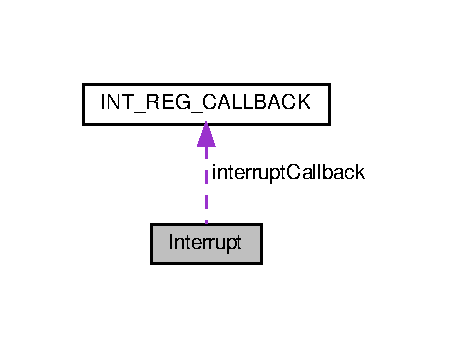
\includegraphics[width=216pt]{classInterrupt__coll__graph}
\end{center}
\end{figure}
\subsection*{Static Public Member Functions}
\begin{DoxyCompactItemize}
\item 
\mbox{\Hypertarget{classInterrupt_a00ff3f6de1e03971a6883b7cb72577e4}\label{classInterrupt_a00ff3f6de1e03971a6883b7cb72577e4}} 
static bool {\bfseries attach\+Interrupt} (uint8\+\_\+t pin, \hyperlink{interrupt_8h_affe9baf0034f4cbb8aec6ed2c42b1676}{I\+N\+T\+\_\+\+E\+D\+GE} edge, \hyperlink{interrupt_8h_af3e04027ddcd2e23670a55888d788d13}{int\+\_\+cb\+\_\+t} $\ast$func)
\item 
\mbox{\Hypertarget{classInterrupt_a3e17ff585a7271441a17f1d5a7a95a47}\label{classInterrupt_a3e17ff585a7271441a17f1d5a7a95a47}} 
static bool {\bfseries deatch\+Interrupt} (uint8\+\_\+t pin)
\end{DoxyCompactItemize}
\subsection*{Static Public Attributes}
\begin{DoxyCompactItemize}
\item 
\mbox{\Hypertarget{classInterrupt_ad98c7ff1c3a116c56b7c67b630967413}\label{classInterrupt_ad98c7ff1c3a116c56b7c67b630967413}} 
static \hyperlink{structINT__REG__CALLBACK}{I\+N\+T\+\_\+\+R\+E\+G\+\_\+\+C\+A\+L\+L\+B\+A\+CK} {\bfseries interrupt\+Callback}
\end{DoxyCompactItemize}
\subsection*{Static Private Member Functions}
\begin{DoxyCompactItemize}
\item 
\mbox{\Hypertarget{classInterrupt_acf51bc7c69619e4ccd95e90ff31aa286}\label{classInterrupt_acf51bc7c69619e4ccd95e90ff31aa286}} 
static void {\bfseries init\+Interrupt} ()
\item 
\mbox{\Hypertarget{classInterrupt_a262ad3f1bb4a5cdf24a356b20d037a56}\label{classInterrupt_a262ad3f1bb4a5cdf24a356b20d037a56}} 
static \hyperlink{interrupt_8h_a530c4d3ebd7cd9fb12aba6242e88d494}{I\+N\+T\+\_\+\+P\+I\+N\+\_\+\+R\+ES} {\bfseries search\+Pin} (uint8\+\_\+t pin, \hyperlink{structPCINT__PIN}{P\+C\+I\+N\+T\+\_\+\+P\+IN} $\ast$\+\_\+pin, \hyperlink{structHW__INT__PIN}{H\+W\+\_\+\+I\+N\+T\+\_\+\+P\+IN} $\ast$\+\_\+pin\+HW)
\end{DoxyCompactItemize}


The documentation for this class was generated from the following files\+:\begin{DoxyCompactItemize}
\item 
\hyperlink{interrupt_8h}{interrupt.\+h}\item 
interrupt.\+cpp\end{DoxyCompactItemize}

\hypertarget{classIPv4}{}\section{I\+Pv4 Class Reference}
\label{classIPv4}\index{I\+Pv4@{I\+Pv4}}


Collaboration diagram for I\+Pv4\+:\nopagebreak
\begin{figure}[H]
\begin{center}
\leavevmode
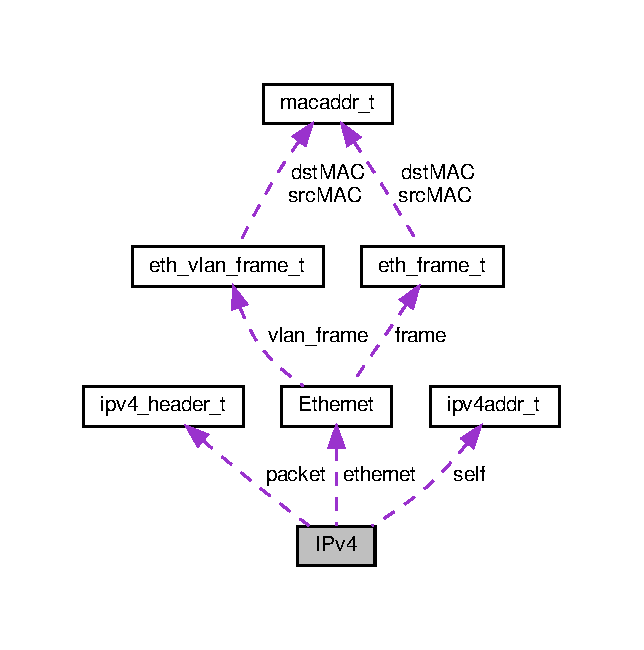
\includegraphics[width=309pt]{classIPv4__coll__graph}
\end{center}
\end{figure}
\subsection*{Public Member Functions}
\begin{DoxyCompactItemize}
\item 
\mbox{\Hypertarget{classIPv4_a1a9cf95c0b539638ccf87ec9540d1f5f}\label{classIPv4_a1a9cf95c0b539638ccf87ec9540d1f5f}} 
void {\bfseries encapsulate} (std\+::vector$<$ u8t $>$ \&payload)
\item 
\mbox{\Hypertarget{classIPv4_ac755be8eb652472e2976200f4c7112da}\label{classIPv4_ac755be8eb652472e2976200f4c7112da}} 
std\+::vector$<$ u8t $>$ {\bfseries decapsulate} (std\+::vector$<$ u8t $>$ \&data)
\item 
\mbox{\Hypertarget{classIPv4_aee57f9b38cf587fd7580324b4e0cf363}\label{classIPv4_aee57f9b38cf587fd7580324b4e0cf363}} 
u32t {\bfseries get\+Src\+Address} ()
\item 
\mbox{\Hypertarget{classIPv4_a4b2067f9ec3bc10827b005a41ab8629c}\label{classIPv4_a4b2067f9ec3bc10827b005a41ab8629c}} 
void {\bfseries set\+Src\+Address} (\hyperlink{unionipv4addr__t}{ipv4addr\+\_\+t} \&ip)
\item 
\mbox{\Hypertarget{classIPv4_a3d00ed1f1cbee5b83110c896b785cf2a}\label{classIPv4_a3d00ed1f1cbee5b83110c896b785cf2a}} 
u32t {\bfseries get\+Dst\+Address} ()
\item 
\mbox{\Hypertarget{classIPv4_afdf051ffbaafe88e789a222f39a75226}\label{classIPv4_afdf051ffbaafe88e789a222f39a75226}} 
void {\bfseries set\+Dst\+Address} (\hyperlink{unionipv4addr__t}{ipv4addr\+\_\+t} \&ip)
\item 
\mbox{\Hypertarget{classIPv4_abd91126dd9d1f07b31e42b7df0d5f210}\label{classIPv4_abd91126dd9d1f07b31e42b7df0d5f210}} 
H\+E\+A\+D\+\_\+\+I\+P\+V4\+\_\+\+P\+R\+O\+T\+O\+C\+OL {\bfseries get\+Protocol} () const
\item 
\mbox{\Hypertarget{classIPv4_ac157b4db97d939fbe2c3f3ae0ed1425a}\label{classIPv4_ac157b4db97d939fbe2c3f3ae0ed1425a}} 
void {\bfseries set\+Protocol} (const H\+E\+A\+D\+\_\+\+I\+P\+V4\+\_\+\+P\+R\+O\+T\+O\+C\+OL \&value)
\item 
\mbox{\Hypertarget{classIPv4_a46bc1d4063db256e32195873bc52ba6a}\label{classIPv4_a46bc1d4063db256e32195873bc52ba6a}} 
char $\ast$ {\bfseries ntoa} (const u32t ip)
\end{DoxyCompactItemize}
\subsection*{Private Member Functions}
\begin{DoxyCompactItemize}
\item 
\mbox{\Hypertarget{classIPv4_a302dbff73ecbbdf99d3552fb996362b9}\label{classIPv4_a302dbff73ecbbdf99d3552fb996362b9}} 
u16t {\bfseries calc\+Header\+Crc} ()
\end{DoxyCompactItemize}
\subsection*{Private Attributes}
\begin{DoxyCompactItemize}
\item 
\mbox{\Hypertarget{classIPv4_a4288e410994ae3a739dc7e2a6aedeb90}\label{classIPv4_a4288e410994ae3a739dc7e2a6aedeb90}} 
\hyperlink{unionipv4addr__t}{ipv4addr\+\_\+t} {\bfseries self}
\item 
\mbox{\Hypertarget{classIPv4_abc94da213c7f9b909a96821315230fbc}\label{classIPv4_abc94da213c7f9b909a96821315230fbc}} 
\hyperlink{structipv4__header__t}{ipv4\+\_\+header\+\_\+t} {\bfseries packet}
\item 
\mbox{\Hypertarget{classIPv4_a0cded8cd68cb45095673e91d3739a15c}\label{classIPv4_a0cded8cd68cb45095673e91d3739a15c}} 
\hyperlink{classEthernet}{Ethernet} {\bfseries ethernet}
\end{DoxyCompactItemize}


The documentation for this class was generated from the following files\+:\begin{DoxyCompactItemize}
\item 
ipv4.\+h\item 
ipv4.\+cpp\end{DoxyCompactItemize}

\hypertarget{structipv4__header__t}{}\section{ipv4\+\_\+header\+\_\+t Struct Reference}
\label{structipv4__header__t}\index{ipv4\+\_\+header\+\_\+t@{ipv4\+\_\+header\+\_\+t}}
\subsection*{Public Attributes}
\begin{DoxyCompactItemize}
\item 
\mbox{\Hypertarget{structipv4__header__t_ac188d1ae5ea19139be084aabea16ecb1}\label{structipv4__header__t_ac188d1ae5ea19139be084aabea16ecb1}} 
\hyperlink{macros_8h_a176a4ab0531a048e0693a4520c550193}{u8t} {\bfseries version}\+:4
\item 
\mbox{\Hypertarget{structipv4__header__t_ac11ce6acd566bf026316c761fc9532fd}\label{structipv4__header__t_ac11ce6acd566bf026316c761fc9532fd}} 
\hyperlink{macros_8h_a176a4ab0531a048e0693a4520c550193}{u8t} {\bfseries header\+Length}\+:4
\item 
\mbox{\Hypertarget{structipv4__header__t_a55f855624993b828721755ec8942256d}\label{structipv4__header__t_a55f855624993b828721755ec8942256d}} 
\hyperlink{macros_8h_a176a4ab0531a048e0693a4520c550193}{u8t} {\bfseries diff\+Services}
\item 
\mbox{\Hypertarget{structipv4__header__t_a3503c52bc9b72749fb422fa108dd15f8}\label{structipv4__header__t_a3503c52bc9b72749fb422fa108dd15f8}} 
\hyperlink{macros_8h_a464a07ed2c6d005d677113cc44750a64}{u32t} {\bfseries total\+\_\+length}
\item 
\mbox{\Hypertarget{structipv4__header__t_a039763ed73f6968b0a6cecf4f144fe85}\label{structipv4__header__t_a039763ed73f6968b0a6cecf4f144fe85}} 
\hyperlink{macros_8h_a590a9a8f7df8fabfac6573e21da1922d}{u16t} {\bfseries identificaton}
\item 
\mbox{\Hypertarget{structipv4__header__t_a7865e9fdc047af71d5bf561256bc5081}\label{structipv4__header__t_a7865e9fdc047af71d5bf561256bc5081}} 
\hyperlink{macros_8h_a176a4ab0531a048e0693a4520c550193}{u8t} {\bfseries flags}\+:3
\item 
\mbox{\Hypertarget{structipv4__header__t_a5b4f68e31a631a875b616d6c389936ce}\label{structipv4__header__t_a5b4f68e31a631a875b616d6c389936ce}} 
\hyperlink{macros_8h_a590a9a8f7df8fabfac6573e21da1922d}{u16t} {\bfseries fragment\+Offset}\+:13
\item 
\mbox{\Hypertarget{structipv4__header__t_a43c20799b97f008f7eb1226329078b89}\label{structipv4__header__t_a43c20799b97f008f7eb1226329078b89}} 
\hyperlink{macros_8h_a176a4ab0531a048e0693a4520c550193}{u8t} {\bfseries T\+TL}
\item 
\mbox{\Hypertarget{structipv4__header__t_abcb115504415c8546c24394f44037f5f}\label{structipv4__header__t_abcb115504415c8546c24394f44037f5f}} 
\hyperlink{macros_8h_a176a4ab0531a048e0693a4520c550193}{u8t} {\bfseries protocol}
\item 
\mbox{\Hypertarget{structipv4__header__t_a056f1d4b637c9ac36f326690ab584ab3}\label{structipv4__header__t_a056f1d4b637c9ac36f326690ab584ab3}} 
\hyperlink{macros_8h_a464a07ed2c6d005d677113cc44750a64}{u32t} {\bfseries header\+C\+RC}
\item 
\mbox{\Hypertarget{structipv4__header__t_ade49e0bd0402fafc2f94d31277ebe6e3}\label{structipv4__header__t_ade49e0bd0402fafc2f94d31277ebe6e3}} 
\hyperlink{macros_8h_a464a07ed2c6d005d677113cc44750a64}{u32t} {\bfseries source\+Address}
\item 
\mbox{\Hypertarget{structipv4__header__t_a2b746f34fa839a18b548f8b950fdab61}\label{structipv4__header__t_a2b746f34fa839a18b548f8b950fdab61}} 
\hyperlink{macros_8h_a464a07ed2c6d005d677113cc44750a64}{u32t} {\bfseries destination\+Address}
\item 
\mbox{\Hypertarget{structipv4__header__t_a86340594c0fd6d27fe9bbeeb129f31f2}\label{structipv4__header__t_a86340594c0fd6d27fe9bbeeb129f31f2}} 
\hyperlink{macros_8h_a176a4ab0531a048e0693a4520c550193}{u8t} {\bfseries option}
\item 
\mbox{\Hypertarget{structipv4__header__t_a3e5bb6d694e89999c96e42576d7a052b}\label{structipv4__header__t_a3e5bb6d694e89999c96e42576d7a052b}} 
\hyperlink{macros_8h_a176a4ab0531a048e0693a4520c550193}{u8t} {\bfseries padding} \mbox{[}3\mbox{]}
\item 
\mbox{\Hypertarget{structipv4__header__t_a6cb0f06ef984e798b7bfe4eeb11fa4d9}\label{structipv4__header__t_a6cb0f06ef984e798b7bfe4eeb11fa4d9}} 
std\+::vector$<$ \hyperlink{macros_8h_a176a4ab0531a048e0693a4520c550193}{u8t} $>$ {\bfseries payload}
\end{DoxyCompactItemize}


The documentation for this struct was generated from the following file\+:\begin{DoxyCompactItemize}
\item 
inet\+\_\+global.\+h\end{DoxyCompactItemize}

\hypertarget{unionipv4addr__t}{}\section{ipv4addr\+\_\+t Union Reference}
\label{unionipv4addr__t}\index{ipv4addr\_t@{ipv4addr\_t}}
\subsection*{Public Attributes}
\begin{DoxyCompactItemize}
\item 
\mbox{\Hypertarget{unionipv4addr__t_ad433218e640ad7a4cfa6382a4edc026d}\label{unionipv4addr__t_ad433218e640ad7a4cfa6382a4edc026d}} 
u8t {\bfseries fields} \mbox{[}4\mbox{]}
\item 
\mbox{\Hypertarget{unionipv4addr__t_a7ad3271285fde5de3a499b380f668851}\label{unionipv4addr__t_a7ad3271285fde5de3a499b380f668851}} 
u32t {\bfseries ip}
\end{DoxyCompactItemize}


The documentation for this union was generated from the following file\+:\begin{DoxyCompactItemize}
\item 
inet\+\_\+global.\+h\end{DoxyCompactItemize}

\hypertarget{structmacaddr__t}{}\section{macaddr\+\_\+t Struct Reference}
\label{structmacaddr__t}\index{macaddr\_t@{macaddr\_t}}
\subsection*{Public Member Functions}
\begin{DoxyCompactItemize}
\item 
\mbox{\Hypertarget{structmacaddr__t_a442a83a92a78c0a1acacbe36e0471728}\label{structmacaddr__t_a442a83a92a78c0a1acacbe36e0471728}} 
{\bfseries macaddr\+\_\+t} (u8t $\ast$mac=nullptr)
\end{DoxyCompactItemize}
\subsection*{Public Attributes}
\begin{DoxyCompactItemize}
\item 
\mbox{\Hypertarget{structmacaddr__t_a3c7dd2e488f6e23119c500482ac3c64a}\label{structmacaddr__t_a3c7dd2e488f6e23119c500482ac3c64a}} 
uint8\+\_\+t {\bfseries mac} \mbox{[}6\mbox{]}
\end{DoxyCompactItemize}


The documentation for this struct was generated from the following file\+:\begin{DoxyCompactItemize}
\item 
inet\+\_\+global.\+h\end{DoxyCompactItemize}

\hypertarget{structMappedPort}{}\section{Mapped\+Port Struct Reference}
\label{structMappedPort}\index{MappedPort@{MappedPort}}


The \mbox{\hyperlink{structMappedPort}{Mapped\+Port}} struct. It\textquotesingle{}s used to manage pins.  




{\ttfamily \#include $<$portmanager.\+h$>$}

\subsection*{Public Attributes}
\begin{DoxyCompactItemize}
\item 
\mbox{\Hypertarget{structMappedPort_a504fc8fe2e91d886ed39d36a3c4e40f8}\label{structMappedPort_a504fc8fe2e91d886ed39d36a3c4e40f8}} 
volatile uint8\+\_\+t $\ast$ \mbox{\hyperlink{structMappedPort_a504fc8fe2e91d886ed39d36a3c4e40f8}{pinx}}
\begin{DoxyCompactList}\small\item\em Is the pointer used to manage a pin. \end{DoxyCompactList}\item 
\mbox{\Hypertarget{structMappedPort_a5a906790bc9881785c9c166c8591dfc2}\label{structMappedPort_a5a906790bc9881785c9c166c8591dfc2}} 
uint8\+\_\+t \mbox{\hyperlink{structMappedPort_a5a906790bc9881785c9c166c8591dfc2}{register\+Bit}}
\begin{DoxyCompactList}\small\item\em The bit into own register. \end{DoxyCompactList}\item 
uint16\+\_\+t \mbox{\hyperlink{structMappedPort_ae73f042b9d9a8a1a87d489525a2ca947}{control\+Bits}}
\begin{DoxyCompactList}\small\item\em Used to get pin functions mode. \end{DoxyCompactList}\end{DoxyCompactItemize}


\subsection{Detailed Description}
The \mbox{\hyperlink{structMappedPort}{Mapped\+Port}} struct. It\textquotesingle{}s used to manage pins. 

\subsection{Member Data Documentation}
\mbox{\Hypertarget{structMappedPort_ae73f042b9d9a8a1a87d489525a2ca947}\label{structMappedPort_ae73f042b9d9a8a1a87d489525a2ca947}} 
\index{MappedPort@{MappedPort}!controlBits@{controlBits}}
\index{controlBits@{controlBits}!MappedPort@{MappedPort}}
\subsubsection{\texorpdfstring{controlBits}{controlBits}}
{\footnotesize\ttfamily Mapped\+Port\+::control\+Bits}



Used to get pin functions mode. 

\begin{DoxyVerb}╔═══════╦══════╦══════╦══════╦══════╦═════╦═══════╦═══╦═══╦═══╦═══╦════════╦═════╦════╗
║ 13    ║ 12   ║ 11   ║ 10   ║ 9    ║ 8   ║ 7     ║ 6 ║ 5 ║ 4 ║ 3 ║ 2      ║ 1   ║ 0  ║
╠═══════╬══════╩══════╩══════╬══════╩═════╬═══════╬═══╩═══╩═══╩═══╬════════╬═════╩════╣
║ isPWM ║ Output Compare Sel ║ Letter Sel ║ isADC ║ ADC_SEL       ║ isUART ║ UART_SEL ║
╚═══════╩════════════════════╩════════════╩═══════╩═══════════════╩════════╩══════════╝
\end{DoxyVerb}
 

The documentation for this struct was generated from the following file\+:\begin{DoxyCompactItemize}
\item 
\mbox{\hyperlink{portmanager_8h}{portmanager.\+h}}\end{DoxyCompactItemize}

\hypertarget{classMasterSPI}{}\section{Master\+S\+PI Class Reference}
\label{classMasterSPI}\index{Master\+S\+PI@{Master\+S\+PI}}


Collaboration diagram for Master\+S\+PI\+:\nopagebreak
\begin{figure}[H]
\begin{center}
\leavevmode
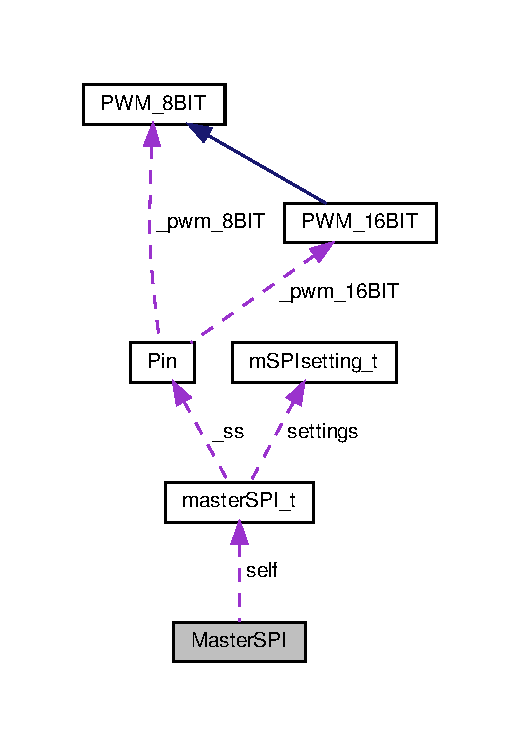
\includegraphics[width=248pt]{classMasterSPI__coll__graph}
\end{center}
\end{figure}
\subsection*{Public Member Functions}
\begin{DoxyCompactItemize}
\item 
\mbox{\Hypertarget{classMasterSPI_abfc56edf4c6f5c60d8f55f4c4a579c75}\label{classMasterSPI_abfc56edf4c6f5c60d8f55f4c4a579c75}} 
{\bfseries Master\+S\+PI} (\hyperlink{structmasterSPI__t}{master\+S\+P\+I\+\_\+t} data, \hyperlink{structmSPIsetting__t}{m\+S\+P\+Isetting\+\_\+t} settings)
\item 
\mbox{\Hypertarget{classMasterSPI_a1e141d3c600973a7fbc20295fd848166}\label{classMasterSPI_a1e141d3c600973a7fbc20295fd848166}} 
void {\bfseries enable} ()
\item 
\mbox{\Hypertarget{classMasterSPI_adae97af990eca4566cec849cb39dd0fc}\label{classMasterSPI_adae97af990eca4566cec849cb39dd0fc}} 
void {\bfseries disable} ()
\item 
\mbox{\Hypertarget{classMasterSPI_a9bdb983b346cc4b03eac1ef30dfc8686}\label{classMasterSPI_a9bdb983b346cc4b03eac1ef30dfc8686}} 
void {\bfseries set\+Clock} (S\+P\+I\+\_\+\+C\+L\+K\+S\+EL clock)
\item 
\mbox{\Hypertarget{classMasterSPI_a21f2d0bfe737d96f628bd70ea7b6514d}\label{classMasterSPI_a21f2d0bfe737d96f628bd70ea7b6514d}} 
S\+P\+I\+\_\+\+C\+L\+K\+S\+EL {\bfseries get\+Clock} ()
\item 
\mbox{\Hypertarget{classMasterSPI_a566f067a1e45eea6705d0973c4cf8862}\label{classMasterSPI_a566f067a1e45eea6705d0973c4cf8862}} 
void {\bfseries set\+Data\+Order} (S\+P\+I\+\_\+\+D\+O\+RD data\+Order)
\item 
\mbox{\Hypertarget{classMasterSPI_af65dc8e666dacce098002f25d8154e4b}\label{classMasterSPI_af65dc8e666dacce098002f25d8154e4b}} 
S\+P\+I\+\_\+\+D\+O\+RD {\bfseries get\+Data\+Order} ()
\item 
\mbox{\Hypertarget{classMasterSPI_a7bd208fd11af5254a31acd9ac17aedcf}\label{classMasterSPI_a7bd208fd11af5254a31acd9ac17aedcf}} 
void {\bfseries set\+Clock\+Polarity} (S\+P\+I\+\_\+\+C\+P\+OL clock\+Polarity)
\item 
\mbox{\Hypertarget{classMasterSPI_abe36df23759ef1ac4ceabf8beb0c87e1}\label{classMasterSPI_abe36df23759ef1ac4ceabf8beb0c87e1}} 
S\+P\+I\+\_\+\+C\+P\+OL {\bfseries get\+Clock\+Polarity} ()
\item 
\mbox{\Hypertarget{classMasterSPI_af62130860321f5d56dbef942ed4dd976}\label{classMasterSPI_af62130860321f5d56dbef942ed4dd976}} 
void {\bfseries set\+Clock\+Phase} (S\+P\+I\+\_\+\+C\+P\+HA clock\+Phase)
\item 
\mbox{\Hypertarget{classMasterSPI_a4ab249c40732baf10c84e679716c06bb}\label{classMasterSPI_a4ab249c40732baf10c84e679716c06bb}} 
S\+P\+I\+\_\+\+C\+P\+HA {\bfseries get\+Clock\+Phase} ()
\item 
\mbox{\Hypertarget{classMasterSPI_a405be54a885e480053d6bed914ae945b}\label{classMasterSPI_a405be54a885e480053d6bed914ae945b}} 
void {\bfseries enable\+Slave} (uint8\+\_\+t slave)
\item 
\mbox{\Hypertarget{classMasterSPI_ab68209dd073458c4d9e67c8fe48f0c23}\label{classMasterSPI_ab68209dd073458c4d9e67c8fe48f0c23}} 
void {\bfseries disable\+Slave} (uint8\+\_\+t slave)
\item 
\mbox{\Hypertarget{classMasterSPI_ab14828b0e7ba5d57b69416592e967827}\label{classMasterSPI_ab14828b0e7ba5d57b69416592e967827}} 
void {\bfseries send} (uint8\+\_\+t data)
\item 
\mbox{\Hypertarget{classMasterSPI_a488585ba1bcc08d0d996351eae1a5846}\label{classMasterSPI_a488585ba1bcc08d0d996351eae1a5846}} 
void {\bfseries send} (uint8\+\_\+t $\ast$buff, size\+\_\+t size)
\item 
\mbox{\Hypertarget{classMasterSPI_a9fb1e852ea7f95416ac3eb3823fde022}\label{classMasterSPI_a9fb1e852ea7f95416ac3eb3823fde022}} 
uint8\+\_\+t {\bfseries receive} ()
\item 
\mbox{\Hypertarget{classMasterSPI_a1ef210d931a745610273733223f813e1}\label{classMasterSPI_a1ef210d931a745610273733223f813e1}} 
void {\bfseries receive} (uint8\+\_\+t $\ast$buff, size\+\_\+t size)
\item 
\mbox{\Hypertarget{classMasterSPI_a6b3659712a73698d618d7ce9e6b7fce0}\label{classMasterSPI_a6b3659712a73698d618d7ce9e6b7fce0}} 
uint8\+\_\+t {\bfseries send\+Receive} (uint8\+\_\+t data)
\item 
\mbox{\Hypertarget{classMasterSPI_a44270af41c0a3a77e6dd3d57248b062c}\label{classMasterSPI_a44270af41c0a3a77e6dd3d57248b062c}} 
void {\bfseries send\+Receive} (uint8\+\_\+t $\ast$dst, uint8\+\_\+t $\ast$src, size\+\_\+t size)
\item 
\mbox{\Hypertarget{classMasterSPI_ab812254b48ad06a1a3d4da3d7dbd577f}\label{classMasterSPI_ab812254b48ad06a1a3d4da3d7dbd577f}} 
bool {\bfseries is\+Initilized\+S\+PI} ()
\end{DoxyCompactItemize}
\subsection*{Private Member Functions}
\begin{DoxyCompactItemize}
\item 
\mbox{\Hypertarget{classMasterSPI_ad1442558b7d3ee172b3529d50854b8bc}\label{classMasterSPI_ad1442558b7d3ee172b3529d50854b8bc}} 
bool {\bfseries slave\+Is\+Valid} (uint8\+\_\+t slave)
\end{DoxyCompactItemize}
\subsection*{Private Attributes}
\begin{DoxyCompactItemize}
\item 
\mbox{\Hypertarget{classMasterSPI_ad92299e347f8e51309afc226daff5677}\label{classMasterSPI_ad92299e347f8e51309afc226daff5677}} 
\hyperlink{structmasterSPI__t}{master\+S\+P\+I\+\_\+t} {\bfseries self}
\end{DoxyCompactItemize}


The documentation for this class was generated from the following files\+:\begin{DoxyCompactItemize}
\item 
\hyperlink{spimaster_8h}{spimaster.\+h}\item 
spimaster.\+cpp\end{DoxyCompactItemize}

\hypertarget{structmasterSPI__t}{}\section{master\+S\+P\+I\+\_\+t Struct Reference}
\label{structmasterSPI__t}\index{masterSPI\_t@{masterSPI\_t}}


Collaboration diagram for master\+S\+P\+I\+\_\+t\+:\nopagebreak
\begin{figure}[H]
\begin{center}
\leavevmode
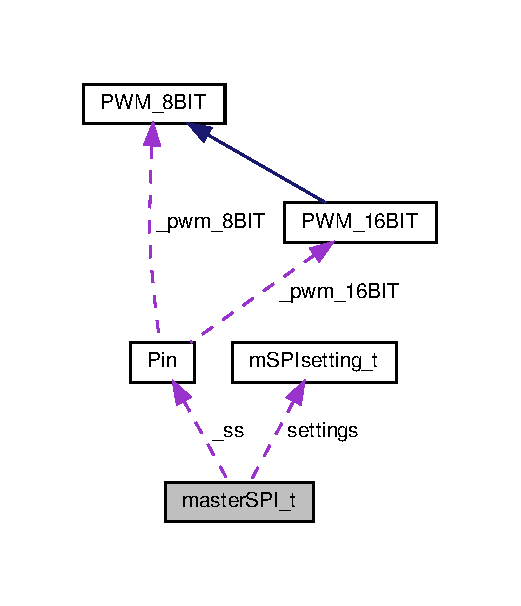
\includegraphics[width=248pt]{structmasterSPI__t__coll__graph}
\end{center}
\end{figure}
\subsection*{Public Member Functions}
\begin{DoxyCompactItemize}
\item 
\mbox{\Hypertarget{structmasterSPI__t_a3344d8520f2e855f5ecf53bfe03415fe}\label{structmasterSPI__t_a3344d8520f2e855f5ecf53bfe03415fe}} 
{\bfseries master\+S\+P\+I\+\_\+t} (volatile uint8\+\_\+t $\ast$pinx=nullptr, \mbox{\hyperlink{classPin}{Pin}} $\ast$miso=nullptr, \mbox{\hyperlink{classPin}{Pin}} $\ast$mosi=nullptr, \mbox{\hyperlink{classPin}{Pin}} $\ast$sck=nullptr, \mbox{\hyperlink{classPin}{Pin}} $\ast$ss=nullptr)
\end{DoxyCompactItemize}
\subsection*{Public Attributes}
\begin{DoxyCompactItemize}
\item 
\mbox{\Hypertarget{structmasterSPI__t_a69f13d6f82316cbad3e05aa1067c25ab}\label{structmasterSPI__t_a69f13d6f82316cbad3e05aa1067c25ab}} 
volatile uint8\+\_\+t $\ast$ {\bfseries P\+I\+Nx}
\item 
\mbox{\Hypertarget{structmasterSPI__t_a24aa73fb35508a28c63f1fad2f3548dc}\label{structmasterSPI__t_a24aa73fb35508a28c63f1fad2f3548dc}} 
volatile uint8\+\_\+t $\ast$ {\bfseries D\+D\+Rx}
\item 
\mbox{\Hypertarget{structmasterSPI__t_a819eae46f1e853b89ac501081cb1c2e9}\label{structmasterSPI__t_a819eae46f1e853b89ac501081cb1c2e9}} 
volatile uint8\+\_\+t $\ast$ {\bfseries P\+O\+R\+Tx}
\item 
\mbox{\Hypertarget{structmasterSPI__t_a9265e0ac3fe401504361a960fce3eb78}\label{structmasterSPI__t_a9265e0ac3fe401504361a960fce3eb78}} 
uint8\+\_\+t {\bfseries bit\+M\+I\+SO}
\item 
\mbox{\Hypertarget{structmasterSPI__t_acfbd932e92c901306860214a154e383b}\label{structmasterSPI__t_acfbd932e92c901306860214a154e383b}} 
uint8\+\_\+t {\bfseries bit\+M\+O\+SI}
\item 
\mbox{\Hypertarget{structmasterSPI__t_af26928ddc81c31b6b66dd473d6c63c4c}\label{structmasterSPI__t_af26928ddc81c31b6b66dd473d6c63c4c}} 
uint8\+\_\+t {\bfseries bit\+S\+CK}
\item 
\mbox{\Hypertarget{structmasterSPI__t_a7238d1be10b3bf5e15fd9786d09b3b3f}\label{structmasterSPI__t_a7238d1be10b3bf5e15fd9786d09b3b3f}} 
uint8\+\_\+t {\bfseries bit\+SS}
\item 
\mbox{\Hypertarget{structmasterSPI__t_a49ce53c491227c03ddb088bf918437d2}\label{structmasterSPI__t_a49ce53c491227c03ddb088bf918437d2}} 
\mbox{\hyperlink{classPin}{Pin}} {\bfseries \+\_\+ss}
\item 
\mbox{\Hypertarget{structmasterSPI__t_ad0195c06fe173b42b66d9169ba1d15df}\label{structmasterSPI__t_ad0195c06fe173b42b66d9169ba1d15df}} 
std\+::vector$<$ \mbox{\hyperlink{classPin}{Pin}} $>$ {\bfseries SS}
\item 
\mbox{\Hypertarget{structmasterSPI__t_ae2c1bb02c7d7b80d2fff99eacf108eb0}\label{structmasterSPI__t_ae2c1bb02c7d7b80d2fff99eacf108eb0}} 
\mbox{\hyperlink{structmSPIsetting__t}{m\+S\+P\+Isetting\+\_\+t}} {\bfseries settings}
\end{DoxyCompactItemize}


The documentation for this struct was generated from the following file\+:\begin{DoxyCompactItemize}
\item 
spimaster.\+h\end{DoxyCompactItemize}

\hypertarget{classMpu6050}{}\section{Mpu6050 Class Reference}
\label{classMpu6050}\index{Mpu6050@{Mpu6050}}


Collaboration diagram for Mpu6050\+:\nopagebreak
\begin{figure}[H]
\begin{center}
\leavevmode
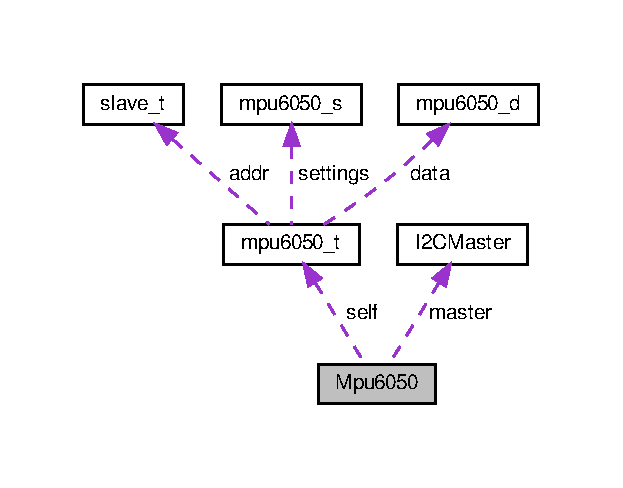
\includegraphics[width=299pt]{classMpu6050__coll__graph}
\end{center}
\end{figure}
\subsection*{Public Member Functions}
\begin{DoxyCompactItemize}
\item 
\mbox{\Hypertarget{classMpu6050_a66c02083300656955c6ab4825a9a2cf7}\label{classMpu6050_a66c02083300656955c6ab4825a9a2cf7}} 
{\bfseries Mpu6050} (\hyperlink{structslave__t}{slave\+\_\+t} addr)
\item 
\mbox{\Hypertarget{classMpu6050_ada44fc04a552a9f0ac78e8406958f372}\label{classMpu6050_ada44fc04a552a9f0ac78e8406958f372}} 
{\bfseries Mpu6050} (uint8\+\_\+t write\+Addr=0x\+D0, uint8\+\_\+t read\+Addr=0x\+D1)
\item 
\mbox{\Hypertarget{classMpu6050_a066832c484d51f19bca711291eb8b6f6}\label{classMpu6050_a066832c484d51f19bca711291eb8b6f6}} 
void {\bfseries wake\+Up} ()
\item 
\mbox{\Hypertarget{classMpu6050_aad083177a7f103792055e0fffdabc99c}\label{classMpu6050_aad083177a7f103792055e0fffdabc99c}} 
void {\bfseries sleep} ()
\item 
\mbox{\Hypertarget{classMpu6050_adff3dea805b3277544f2a1055ab88b82}\label{classMpu6050_adff3dea805b3277544f2a1055ab88b82}} 
\hyperlink{structmpu6050__d}{mpu6050\+\_\+d} {\bfseries get\+Raw\+Data} ()
\item 
\mbox{\Hypertarget{classMpu6050_a454db86b0f6deaec49bec03104fbc36b}\label{classMpu6050_a454db86b0f6deaec49bec03104fbc36b}} 
\hyperlink{structmpu6050__f}{mpu6050\+\_\+f} {\bfseries get\+Data\+Fixed} (T\+E\+M\+P\+\_\+\+U\+N\+I\+TS unit)
\item 
\mbox{\Hypertarget{classMpu6050_aec4a6223578c5b5ec218c549b529acfc}\label{classMpu6050_aec4a6223578c5b5ec218c549b529acfc}} 
void {\bfseries set\+Accel\+Range} (A\+C\+C\+E\+L\+\_\+\+R\+A\+N\+GE range=M\+P\+U6050\+\_\+\+R\+A\+N\+G\+E\+\_\+2G)
\item 
\mbox{\Hypertarget{classMpu6050_a09ea34d6c38da2353cb7162404f08da6}\label{classMpu6050_a09ea34d6c38da2353cb7162404f08da6}} 
A\+C\+C\+E\+L\+\_\+\+R\+A\+N\+GE {\bfseries get\+Accel\+Range} ()
\item 
\mbox{\Hypertarget{classMpu6050_a7b9f3b74955abf148a7f7e9a2de00819}\label{classMpu6050_a7b9f3b74955abf148a7f7e9a2de00819}} 
void {\bfseries set\+Gyro\+Range} (G\+Y\+R\+O\+\_\+\+R\+A\+N\+GE range=M\+P\+U6050\+\_\+\+G\+Y\+R\+O\+\_\+\+F\+S\+\_\+250)
\item 
\mbox{\Hypertarget{classMpu6050_a97ff9e30c5af6767b44cce16f317c877}\label{classMpu6050_a97ff9e30c5af6767b44cce16f317c877}} 
G\+Y\+R\+O\+\_\+\+R\+A\+N\+GE {\bfseries get\+Gyro\+Range} ()
\end{DoxyCompactItemize}
\subsection*{Private Attributes}
\begin{DoxyCompactItemize}
\item 
\mbox{\Hypertarget{classMpu6050_a268012468e495b0888a659dc0458a72c}\label{classMpu6050_a268012468e495b0888a659dc0458a72c}} 
\hyperlink{classI2CMaster}{I2\+C\+Master} {\bfseries master}
\item 
\mbox{\Hypertarget{classMpu6050_a53fb7f46e549c2fc2a40a3fcca31825f}\label{classMpu6050_a53fb7f46e549c2fc2a40a3fcca31825f}} 
\hyperlink{structmpu6050__t}{mpu6050\+\_\+t} {\bfseries self}
\end{DoxyCompactItemize}


The documentation for this class was generated from the following files\+:\begin{DoxyCompactItemize}
\item 
mpu6050.\+h\item 
mpu6050.\+cpp\end{DoxyCompactItemize}

\hypertarget{structmpu6050__d}{}\section{mpu6050\+\_\+d Struct Reference}
\label{structmpu6050__d}\index{mpu6050\_d@{mpu6050\_d}}
\subsection*{Public Attributes}
\begin{DoxyCompactItemize}
\item 
\mbox{\Hypertarget{structmpu6050__d_adb7ccae71a0c5e7f258586d0495c6a8c}\label{structmpu6050__d_adb7ccae71a0c5e7f258586d0495c6a8c}} 
int16\+\_\+t {\bfseries accelX}
\item 
\mbox{\Hypertarget{structmpu6050__d_aaa5222f3976416bcae0e75a9ba65f0fe}\label{structmpu6050__d_aaa5222f3976416bcae0e75a9ba65f0fe}} 
int16\+\_\+t {\bfseries accelY}
\item 
\mbox{\Hypertarget{structmpu6050__d_a0fdcaed0c39c82e43beb78ccb49c47f2}\label{structmpu6050__d_a0fdcaed0c39c82e43beb78ccb49c47f2}} 
int16\+\_\+t {\bfseries accelZ}
\item 
\mbox{\Hypertarget{structmpu6050__d_ad9660eb6bd1f5d93fd06b8d8f8edbfeb}\label{structmpu6050__d_ad9660eb6bd1f5d93fd06b8d8f8edbfeb}} 
int16\+\_\+t {\bfseries temp}
\item 
\mbox{\Hypertarget{structmpu6050__d_a2c4aa4ef6faddb414f6a638a45d5f634}\label{structmpu6050__d_a2c4aa4ef6faddb414f6a638a45d5f634}} 
int16\+\_\+t {\bfseries gyroX}
\item 
\mbox{\Hypertarget{structmpu6050__d_aae7232a3273a9b40ab0b97a18cb42451}\label{structmpu6050__d_aae7232a3273a9b40ab0b97a18cb42451}} 
int16\+\_\+t {\bfseries gyroY}
\item 
\mbox{\Hypertarget{structmpu6050__d_a5e65eb26d9829b2fff3eeb96823f0fa1}\label{structmpu6050__d_a5e65eb26d9829b2fff3eeb96823f0fa1}} 
int16\+\_\+t {\bfseries gyroZ}
\end{DoxyCompactItemize}


The documentation for this struct was generated from the following file\+:\begin{DoxyCompactItemize}
\item 
mpu6050.\+h\end{DoxyCompactItemize}

\hypertarget{structmpu6050__f}{}\section{mpu6050\+\_\+f Struct Reference}
\label{structmpu6050__f}\index{mpu6050\_f@{mpu6050\_f}}
\subsection*{Public Attributes}
\begin{DoxyCompactItemize}
\item 
\mbox{\Hypertarget{structmpu6050__f_ae1a231d8c1f6e9774d139f86827e66e9}\label{structmpu6050__f_ae1a231d8c1f6e9774d139f86827e66e9}} 
float {\bfseries accelX}
\item 
\mbox{\Hypertarget{structmpu6050__f_a1621b7a2d56e6c51e43019fe3c0b9033}\label{structmpu6050__f_a1621b7a2d56e6c51e43019fe3c0b9033}} 
float {\bfseries accelY}
\item 
\mbox{\Hypertarget{structmpu6050__f_a0cddb44272fc95b87c8fb19caf59d4ac}\label{structmpu6050__f_a0cddb44272fc95b87c8fb19caf59d4ac}} 
float {\bfseries accelZ}
\item 
\mbox{\Hypertarget{structmpu6050__f_a6111a88fd6044126275b43e88be5bedc}\label{structmpu6050__f_a6111a88fd6044126275b43e88be5bedc}} 
float {\bfseries temp}
\item 
\mbox{\Hypertarget{structmpu6050__f_a800cead01d2de6ac814684a145ec7c53}\label{structmpu6050__f_a800cead01d2de6ac814684a145ec7c53}} 
float {\bfseries gyroX}
\item 
\mbox{\Hypertarget{structmpu6050__f_abc55afc127c40b7797bef8d4965b8939}\label{structmpu6050__f_abc55afc127c40b7797bef8d4965b8939}} 
float {\bfseries gyroY}
\item 
\mbox{\Hypertarget{structmpu6050__f_a7c3f52a114e6417080ebdbb3d6560a1a}\label{structmpu6050__f_a7c3f52a114e6417080ebdbb3d6560a1a}} 
float {\bfseries gyroZ}
\end{DoxyCompactItemize}


The documentation for this struct was generated from the following file\+:\begin{DoxyCompactItemize}
\item 
mpu6050.\+h\end{DoxyCompactItemize}

\hypertarget{structmpu6050__s}{}\section{mpu6050\+\_\+s Struct Reference}
\label{structmpu6050__s}\index{mpu6050\+\_\+s@{mpu6050\+\_\+s}}
\subsection*{Public Member Functions}
\begin{DoxyCompactItemize}
\item 
\mbox{\Hypertarget{structmpu6050__s_ab8ff10bcdf8741b34b5fa0d44d8d444c}\label{structmpu6050__s_ab8ff10bcdf8741b34b5fa0d44d8d444c}} 
{\bfseries mpu6050\+\_\+s} (A\+C\+C\+E\+L\+\_\+\+R\+A\+N\+GE accel=M\+P\+U6050\+\_\+\+R\+A\+N\+G\+E\+\_\+2G, G\+Y\+R\+O\+\_\+\+R\+A\+N\+GE gyro=M\+P\+U6050\+\_\+\+G\+Y\+R\+O\+\_\+\+F\+S\+\_\+250)
\end{DoxyCompactItemize}
\subsection*{Public Attributes}
\begin{DoxyCompactItemize}
\item 
\mbox{\Hypertarget{structmpu6050__s_ad31e74a1edf8e3a6259925c87fc8043e}\label{structmpu6050__s_ad31e74a1edf8e3a6259925c87fc8043e}} 
uint8\+\_\+t {\bfseries accel\+Cfg}
\item 
\mbox{\Hypertarget{structmpu6050__s_a2e8ba692a704c815ce6e4c6288b64787}\label{structmpu6050__s_a2e8ba692a704c815ce6e4c6288b64787}} 
uint8\+\_\+t {\bfseries gyro\+Cfg}
\end{DoxyCompactItemize}


The documentation for this struct was generated from the following file\+:\begin{DoxyCompactItemize}
\item 
mpu6050.\+h\end{DoxyCompactItemize}

\hypertarget{structmpu6050__t}{}\section{mpu6050\+\_\+t Struct Reference}
\label{structmpu6050__t}\index{mpu6050\+\_\+t@{mpu6050\+\_\+t}}


Collaboration diagram for mpu6050\+\_\+t\+:\nopagebreak
\begin{figure}[H]
\begin{center}
\leavevmode
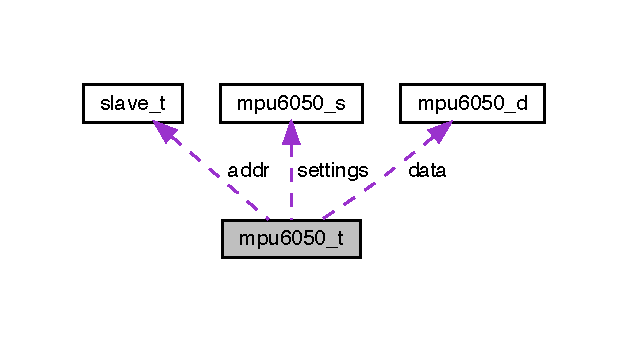
\includegraphics[width=299pt]{structmpu6050__t__coll__graph}
\end{center}
\end{figure}
\subsection*{Public Member Functions}
\begin{DoxyCompactItemize}
\item 
\mbox{\Hypertarget{structmpu6050__t_ae66ee931655d40f389f45fa2bd652dbf}\label{structmpu6050__t_ae66ee931655d40f389f45fa2bd652dbf}} 
{\bfseries mpu6050\+\_\+t} (\hyperlink{structslave__t}{slave\+\_\+t} addr=\hyperlink{structslave__t}{slave\+\_\+t}())
\end{DoxyCompactItemize}
\subsection*{Public Attributes}
\begin{DoxyCompactItemize}
\item 
\mbox{\Hypertarget{structmpu6050__t_a61f3fb7626fd4df7fe919da15b61f400}\label{structmpu6050__t_a61f3fb7626fd4df7fe919da15b61f400}} 
\hyperlink{structslave__t}{slave\+\_\+t} {\bfseries addr}
\item 
\mbox{\Hypertarget{structmpu6050__t_ad9d6c6a1e71d62ebffdbf123aafe009e}\label{structmpu6050__t_ad9d6c6a1e71d62ebffdbf123aafe009e}} 
\hyperlink{structmpu6050__d}{mpu6050\+\_\+d} {\bfseries data}
\item 
\mbox{\Hypertarget{structmpu6050__t_a185513b1c965c430645d75eecf5a401d}\label{structmpu6050__t_a185513b1c965c430645d75eecf5a401d}} 
\hyperlink{structmpu6050__s}{mpu6050\+\_\+s} {\bfseries settings}
\end{DoxyCompactItemize}


The documentation for this struct was generated from the following file\+:\begin{DoxyCompactItemize}
\item 
mpu6050.\+h\end{DoxyCompactItemize}

\hypertarget{structmSPIsetting__t}{}\section{m\+S\+P\+Isetting\+\_\+t Struct Reference}
\label{structmSPIsetting__t}\index{m\+S\+P\+Isetting\+\_\+t@{m\+S\+P\+Isetting\+\_\+t}}
\subsection*{Public Member Functions}
\begin{DoxyCompactItemize}
\item 
\mbox{\Hypertarget{structmSPIsetting__t_a8e24b798a3f9dcd4f90fadffbcab0503}\label{structmSPIsetting__t_a8e24b798a3f9dcd4f90fadffbcab0503}} 
{\bfseries m\+S\+P\+Isetting\+\_\+t} (S\+P\+I\+\_\+\+C\+L\+K\+S\+EL clock\+Sel=F\+O\+S\+C\+\_\+\+B\+Y\+\_\+4, S\+P\+I\+\_\+\+D\+O\+RD data\+Order=M\+S\+B\+\_\+\+F\+I\+R\+ST, S\+P\+I\+\_\+\+C\+P\+OL clock\+Polarity=L\+R\+\_\+\+TF, S\+P\+I\+\_\+\+C\+P\+HA clock\+Phase=L\+S\+\_\+\+TP)
\end{DoxyCompactItemize}
\subsection*{Public Attributes}
\begin{DoxyCompactItemize}
\item 
\mbox{\Hypertarget{structmSPIsetting__t_a808514c1d694629406dbafc8d09d6aac}\label{structmSPIsetting__t_a808514c1d694629406dbafc8d09d6aac}} 
S\+P\+I\+\_\+\+C\+L\+K\+S\+EL {\bfseries \+\_\+clock}
\item 
\mbox{\Hypertarget{structmSPIsetting__t_a8de7023e2f95faed221ee03a3cf5dd93}\label{structmSPIsetting__t_a8de7023e2f95faed221ee03a3cf5dd93}} 
S\+P\+I\+\_\+\+D\+O\+RD {\bfseries \+\_\+data\+Order}
\item 
\mbox{\Hypertarget{structmSPIsetting__t_aa831f0b03d1dfad178c75dc2d4f70904}\label{structmSPIsetting__t_aa831f0b03d1dfad178c75dc2d4f70904}} 
S\+P\+I\+\_\+\+C\+P\+OL {\bfseries \+\_\+clock\+Polarity}
\item 
\mbox{\Hypertarget{structmSPIsetting__t_ae5bee01044abda654f22370844528d21}\label{structmSPIsetting__t_ae5bee01044abda654f22370844528d21}} 
S\+P\+I\+\_\+\+C\+P\+HA {\bfseries \+\_\+clock\+Phase}
\end{DoxyCompactItemize}


The documentation for this struct was generated from the following file\+:\begin{DoxyCompactItemize}
\item 
\hyperlink{spimaster_8h}{spimaster.\+h}\end{DoxyCompactItemize}

\hypertarget{structPCINT__PIN}{}\section{P\+C\+I\+N\+T\+\_\+\+P\+IN Struct Reference}
\label{structPCINT__PIN}\index{P\+C\+I\+N\+T\+\_\+\+P\+IN@{P\+C\+I\+N\+T\+\_\+\+P\+IN}}


The \hyperlink{structPCINT__PIN}{P\+C\+I\+N\+T\+\_\+\+P\+IN} struct.  




{\ttfamily \#include $<$interrupt.\+h$>$}

\subsection*{Public Attributes}
\begin{DoxyCompactItemize}
\item 
\mbox{\Hypertarget{structPCINT__PIN_a2496d6cb8626cb2f59cbce2275c955f7}\label{structPCINT__PIN_a2496d6cb8626cb2f59cbce2275c955f7}} 
uint8\+\_\+t {\bfseries mapped\+Pin}
\item 
\mbox{\Hypertarget{structPCINT__PIN_afc86dc0ea0cd5858b9bd39354192ef0e}\label{structPCINT__PIN_afc86dc0ea0cd5858b9bd39354192ef0e}} 
uint8\+\_\+t {\bfseries P\+C\+I\+N\+Tx\+\_\+vect}
\item 
\mbox{\Hypertarget{structPCINT__PIN_a365ae7574c175d0e95b17e72f6d10d14}\label{structPCINT__PIN_a365ae7574c175d0e95b17e72f6d10d14}} 
uint8\+\_\+t {\bfseries P\+C\+I\+N\+Tx}
\item 
\mbox{\Hypertarget{structPCINT__PIN_a86cd558d3cb07e08e09aa5b4fc764a6b}\label{structPCINT__PIN_a86cd558d3cb07e08e09aa5b4fc764a6b}} 
volatile \hyperlink{interrupt_8h_af3e04027ddcd2e23670a55888d788d13}{int\+\_\+cb\+\_\+t} $\ast$$\ast$ {\bfseries interrupt\+Callback}
\item 
\mbox{\Hypertarget{structPCINT__PIN_ac80a352adca1ee695bd338be6e3828e3}\label{structPCINT__PIN_ac80a352adca1ee695bd338be6e3828e3}} 
\hyperlink{interrupt_8h_affe9baf0034f4cbb8aec6ed2c42b1676}{I\+N\+T\+\_\+\+E\+D\+GE} $\ast$ {\bfseries px\+\_\+edge}
\end{DoxyCompactItemize}


\subsection{Detailed Description}
The \hyperlink{structPCINT__PIN}{P\+C\+I\+N\+T\+\_\+\+P\+IN} struct. 

The documentation for this struct was generated from the following file\+:\begin{DoxyCompactItemize}
\item 
\hyperlink{interrupt_8h}{interrupt.\+h}\end{DoxyCompactItemize}

\hypertarget{classPin}{}\section{Pin Class Reference}
\label{classPin}\index{Pin@{Pin}}


The \mbox{\hyperlink{classPin}{Pin}} class.  




{\ttfamily \#include $<$portmanager.\+h$>$}



Collaboration diagram for Pin\+:\nopagebreak
\begin{figure}[H]
\begin{center}
\leavevmode
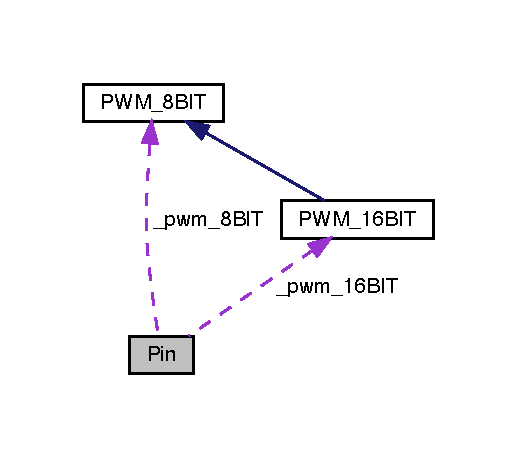
\includegraphics[width=248pt]{classPin__coll__graph}
\end{center}
\end{figure}
\subsection*{Public Member Functions}
\begin{DoxyCompactItemize}
\item 
\mbox{\Hypertarget{classPin_a5a77b8b0c99771c11582f0a011496e6b}\label{classPin_a5a77b8b0c99771c11582f0a011496e6b}} 
{\bfseries Pin} (uint8\+\_\+t port\+No, \mbox{\hyperlink{portmanager_8h_a63d6a5e91a2b1a4156b6c0466f828554}{D\+D\+Rx}} direction)
\item 
\mbox{\Hypertarget{classPin_ae562d4913700a9af64086bc0bad95a28}\label{classPin_ae562d4913700a9af64086bc0bad95a28}} 
void {\bfseries on} ()
\item 
\mbox{\Hypertarget{classPin_a2488d5db01d0bae6d5fe8932b39d3bbe}\label{classPin_a2488d5db01d0bae6d5fe8932b39d3bbe}} 
void {\bfseries set\+State} (bool stat=true)
\item 
\mbox{\Hypertarget{classPin_aa568e83b313f1b9f66bb50f66f18e62c}\label{classPin_aa568e83b313f1b9f66bb50f66f18e62c}} 
void {\bfseries off} ()
\item 
\mbox{\Hypertarget{classPin_a5ecffd86fb366af5ff559faf82a1fc81}\label{classPin_a5ecffd86fb366af5ff559faf82a1fc81}} 
void {\bfseries toggle} ()
\item 
\mbox{\Hypertarget{classPin_a49a4bc8df0fad82b4799fa19da708f12}\label{classPin_a49a4bc8df0fad82b4799fa19da708f12}} 
void {\bfseries set\+Direction} (\mbox{\hyperlink{portmanager_8h_a63d6a5e91a2b1a4156b6c0466f828554}{D\+D\+Rx}} direction)
\item 
\mbox{\Hypertarget{classPin_ae3b0862a7ec9b11f7a8986024669e25a}\label{classPin_ae3b0862a7ec9b11f7a8986024669e25a}} 
bool {\bfseries set\+P\+WM} (uint32\+\_\+t freq, uint8\+\_\+t duty=50)
\item 
\mbox{\Hypertarget{classPin_a938a229474b8319ced9edbad488d6157}\label{classPin_a938a229474b8319ced9edbad488d6157}} 
bool {\bfseries set\+Duty} (uint8\+\_\+t duty)
\item 
\mbox{\Hypertarget{classPin_a8610548d2ab0b531e4e0697ca09aeb0c}\label{classPin_a8610548d2ab0b531e4e0697ca09aeb0c}} 
bool {\bfseries set\+Freq} (uint16\+\_\+t freq)
\item 
\mbox{\Hypertarget{classPin_a4ea18c4f3780b3af59406be5d0b5a176}\label{classPin_a4ea18c4f3780b3af59406be5d0b5a176}} 
bool {\bfseries stop\+P\+WM} ()
\item 
\mbox{\Hypertarget{classPin_ae04006b8dc5d6fb25ff4e2a781ba047d}\label{classPin_ae04006b8dc5d6fb25ff4e2a781ba047d}} 
bool {\bfseries digital\+Read} ()
\item 
\mbox{\Hypertarget{classPin_ac678e5fd7f7bc33260eb909178e17367}\label{classPin_ac678e5fd7f7bc33260eb909178e17367}} 
uint16\+\_\+t {\bfseries analog\+Read} (\+\_\+\+A\+D\+M\+UX v\+Ref=A\+V\+CC, \+\_\+\+A\+D\+C\+S\+R\+A\+\_\+\+P\+R\+E\+S\+C\+A\+L\+ER prescaler=F\+\_\+\+C\+P\+U\+\_\+\+B\+Y\+\_\+128, \+\_\+\+A\+D\+C\+S\+R\+B\+\_\+\+A\+U\+T\+O\+T\+R\+I\+G\+G\+ER auto\+Trigger=F\+R\+E\+E\+\_\+\+R\+U\+N\+N\+I\+N\+G\+\_\+\+M\+O\+DE)
\item 
\mbox{\Hypertarget{classPin_aa81249603376710b26f6e803db46658e}\label{classPin_aa81249603376710b26f6e803db46658e}} 
void {\bfseries get\+Pin\+Data} ()
\item 
uint8\+\_\+t \mbox{\hyperlink{classPin_aaad2c2cc8ccda03ffe9c07e12323cf4d}{get\+Pin\+Number}} ()
\begin{DoxyCompactList}\small\item\em get\+Pin\+Number \end{DoxyCompactList}\item 
uint8\+\_\+t \mbox{\hyperlink{classPin_a5a9c1d0f1937b7083779ca4afba2a607}{get\+P\+WM}} ()
\begin{DoxyCompactList}\small\item\em get\+P\+WM \end{DoxyCompactList}\item 
uint8\+\_\+t \mbox{\hyperlink{classPin_af7d88df8c24769198ee8e022ce0ed0fd}{get\+Register\+Bit}} ()
\begin{DoxyCompactList}\small\item\em get\+Register\+Bit \end{DoxyCompactList}\item 
volatile uint8\+\_\+t $\ast$ \mbox{\hyperlink{classPin_ae2d4f832b081cd2d188151a0c4589f8d}{get\+P\+I\+Nx\+Addr}} ()
\begin{DoxyCompactList}\small\item\em get\+P\+I\+Nx\+Addr \end{DoxyCompactList}\end{DoxyCompactItemize}
\subsection*{Private Member Functions}
\begin{DoxyCompactItemize}
\item 
\mbox{\Hypertarget{classPin_a6a094c4d39ce02a525e77d1951001b53}\label{classPin_a6a094c4d39ce02a525e77d1951001b53}} 
uint16\+\_\+t {\bfseries calculate\+Ticks} (uint32\+\_\+t freq)
\end{DoxyCompactItemize}
\subsection*{Private Attributes}
\begin{DoxyCompactItemize}
\item 
\mbox{\Hypertarget{classPin_a07ee57af89974777d3839df8a13e1791}\label{classPin_a07ee57af89974777d3839df8a13e1791}} 
volatile uint8\+\_\+t $\ast$ {\bfseries \+\_\+ddrx}
\item 
\mbox{\Hypertarget{classPin_a6bad8a39ce0aece01804bf34474a8a24}\label{classPin_a6bad8a39ce0aece01804bf34474a8a24}} 
volatile uint8\+\_\+t $\ast$ {\bfseries \+\_\+portx}
\item 
\mbox{\Hypertarget{classPin_ad36da0eaefb41596bb204bbe489c5599}\label{classPin_ad36da0eaefb41596bb204bbe489c5599}} 
volatile uint8\+\_\+t $\ast$ {\bfseries \+\_\+pinx}
\item 
\mbox{\Hypertarget{classPin_a38f8a9dd584cf216ab48f4524b6f7808}\label{classPin_a38f8a9dd584cf216ab48f4524b6f7808}} 
uint16\+\_\+t {\bfseries channel} = 65535
\item 
\mbox{\Hypertarget{classPin_abd8ffe1c180d2e91cae0567bd7562192}\label{classPin_abd8ffe1c180d2e91cae0567bd7562192}} 
uint8\+\_\+t {\bfseries \+\_\+register\+Bit}
\item 
\mbox{\Hypertarget{classPin_a58fa22db3e90c1a048446df1fa0781c9}\label{classPin_a58fa22db3e90c1a048446df1fa0781c9}} 
uint8\+\_\+t {\bfseries \+\_\+local\+\_\+ctrl\+\_\+bits}
\item 
\mbox{\Hypertarget{classPin_a948a3306a825241abc9634e7d477511a}\label{classPin_a948a3306a825241abc9634e7d477511a}} 
\mbox{\hyperlink{structPWM__16BIT}{P\+W\+M\+\_\+16\+B\+IT}} {\bfseries \+\_\+pwm\+\_\+16\+B\+IT}
\item 
\mbox{\Hypertarget{classPin_a94fc11a6e7aea0f84844b8b3627c38b6}\label{classPin_a94fc11a6e7aea0f84844b8b3627c38b6}} 
\mbox{\hyperlink{structPWM__8BIT}{P\+W\+M\+\_\+8\+B\+IT}} {\bfseries \+\_\+pwm\+\_\+8\+B\+IT}
\item 
\mbox{\Hypertarget{classPin_a8c83fc94d50888134e19fd3c30fc8184}\label{classPin_a8c83fc94d50888134e19fd3c30fc8184}} 
uint16\+\_\+t {\bfseries \+\_\+freq\+\_\+pwm}
\item 
\mbox{\Hypertarget{classPin_a0b0f93214d2c2fd6df6e94b931a63674}\label{classPin_a0b0f93214d2c2fd6df6e94b931a63674}} 
uint16\+\_\+t {\bfseries \+\_\+duty\+\_\+pwm}
\item 
\mbox{\Hypertarget{classPin_ad1b2636ee51b9eea404113295a17e2d7}\label{classPin_ad1b2636ee51b9eea404113295a17e2d7}} 
uint16\+\_\+t {\bfseries \+\_\+control\+Bits}
\item 
\mbox{\Hypertarget{classPin_ae83866782be29ac99476647e3ef26f40}\label{classPin_ae83866782be29ac99476647e3ef26f40}} 
uint8\+\_\+t {\bfseries \+\_\+pin\+Number}
\end{DoxyCompactItemize}


\subsection{Detailed Description}
The \mbox{\hyperlink{classPin}{Pin}} class. 

\subsection{Member Function Documentation}
\mbox{\Hypertarget{classPin_aaad2c2cc8ccda03ffe9c07e12323cf4d}\label{classPin_aaad2c2cc8ccda03ffe9c07e12323cf4d}} 
\index{Pin@{Pin}!getPinNumber@{getPinNumber}}
\index{getPinNumber@{getPinNumber}!Pin@{Pin}}
\subsubsection{\texorpdfstring{getPinNumber()}{getPinNumber()}}
{\footnotesize\ttfamily uint8\+\_\+t Pin\+::get\+Pin\+Number (\begin{DoxyParamCaption}{ }\end{DoxyParamCaption})}



get\+Pin\+Number 

\begin{DoxyReturn}{Returns}
Number of mapped pin into the board 
\end{DoxyReturn}
\mbox{\Hypertarget{classPin_ae2d4f832b081cd2d188151a0c4589f8d}\label{classPin_ae2d4f832b081cd2d188151a0c4589f8d}} 
\index{Pin@{Pin}!getPINxAddr@{getPINxAddr}}
\index{getPINxAddr@{getPINxAddr}!Pin@{Pin}}
\subsubsection{\texorpdfstring{getPINxAddr()}{getPINxAddr()}}
{\footnotesize\ttfamily volatile uint8\+\_\+t $\ast$ Pin\+::get\+P\+I\+Nx\+Addr (\begin{DoxyParamCaption}{ }\end{DoxyParamCaption})}



get\+P\+I\+Nx\+Addr 

\begin{DoxyReturn}{Returns}
Mapped address of P\+I\+Nx 
\end{DoxyReturn}
\mbox{\Hypertarget{classPin_a5a9c1d0f1937b7083779ca4afba2a607}\label{classPin_a5a9c1d0f1937b7083779ca4afba2a607}} 
\index{Pin@{Pin}!getPWM@{getPWM}}
\index{getPWM@{getPWM}!Pin@{Pin}}
\subsubsection{\texorpdfstring{getPWM()}{getPWM()}}
{\footnotesize\ttfamily uint8\+\_\+t Pin\+::get\+P\+WM (\begin{DoxyParamCaption}{ }\end{DoxyParamCaption})}



get\+P\+WM 

\begin{DoxyReturn}{Returns}
Percentage of duty cycle. Range \+: 0\% -\/ 100\% 
\end{DoxyReturn}
\mbox{\Hypertarget{classPin_af7d88df8c24769198ee8e022ce0ed0fd}\label{classPin_af7d88df8c24769198ee8e022ce0ed0fd}} 
\index{Pin@{Pin}!getRegisterBit@{getRegisterBit}}
\index{getRegisterBit@{getRegisterBit}!Pin@{Pin}}
\subsubsection{\texorpdfstring{getRegisterBit()}{getRegisterBit()}}
{\footnotesize\ttfamily uint8\+\_\+t Pin\+::get\+Register\+Bit (\begin{DoxyParamCaption}{ }\end{DoxyParamCaption})}



get\+Register\+Bit 

\begin{DoxyReturn}{Returns}
Bits into own register 
\end{DoxyReturn}


The documentation for this class was generated from the following files\+:\begin{DoxyCompactItemize}
\item 
\mbox{\hyperlink{portmanager_8h}{portmanager.\+h}}\item 
portmanager.\+cpp\end{DoxyCompactItemize}

\hypertarget{structPWM__16BIT}{}\section{P\+W\+M\+\_\+16\+B\+IT Struct Reference}
\label{structPWM__16BIT}\index{P\+W\+M\+\_\+16\+B\+IT@{P\+W\+M\+\_\+16\+B\+IT}}


The \hyperlink{structPWM__16BIT}{P\+W\+M\+\_\+16\+B\+IT} struct.  




{\ttfamily \#include $<$portmanager.\+h$>$}



Inheritance diagram for P\+W\+M\+\_\+16\+B\+IT\+:\nopagebreak
\begin{figure}[H]
\begin{center}
\leavevmode
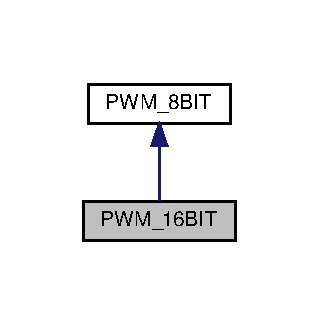
\includegraphics[width=153pt]{structPWM__16BIT__inherit__graph}
\end{center}
\end{figure}


Collaboration diagram for P\+W\+M\+\_\+16\+B\+IT\+:\nopagebreak
\begin{figure}[H]
\begin{center}
\leavevmode
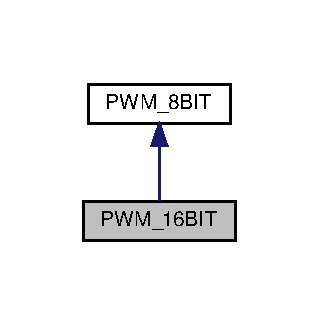
\includegraphics[width=153pt]{structPWM__16BIT__coll__graph}
\end{center}
\end{figure}
\subsection*{Public Attributes}
\begin{DoxyCompactItemize}
\item 
\mbox{\Hypertarget{structPWM__16BIT_aed58d52d5a361e85b19d584d9b59f1b9}\label{structPWM__16BIT_aed58d52d5a361e85b19d584d9b59f1b9}} 
volatile uint8\+\_\+t $\ast$ {\bfseries T\+C\+C\+RxC} = (volatile uint8\+\_\+t $\ast$)0x\+FF
\item 
\mbox{\Hypertarget{structPWM__16BIT_a6e5ea7c07d0fa0f6970bbfe9c2a11677}\label{structPWM__16BIT_a6e5ea7c07d0fa0f6970bbfe9c2a11677}} 
volatile uint8\+\_\+t $\ast$ {\bfseries I\+C\+Rx} = (volatile uint8\+\_\+t $\ast$)0x\+FF
\end{DoxyCompactItemize}


\subsection{Detailed Description}
The \hyperlink{structPWM__16BIT}{P\+W\+M\+\_\+16\+B\+IT} struct. 

The documentation for this struct was generated from the following file\+:\begin{DoxyCompactItemize}
\item 
\hyperlink{portmanager_8h}{portmanager.\+h}\end{DoxyCompactItemize}

\hypertarget{structPWM__8BIT}{}\section{P\+W\+M\+\_\+8\+B\+IT Struct Reference}
\label{structPWM__8BIT}\index{P\+W\+M\+\_\+8\+B\+IT@{P\+W\+M\+\_\+8\+B\+IT}}


The \hyperlink{structPWM__8BIT}{P\+W\+M\+\_\+8\+B\+IT} struct.  




{\ttfamily \#include $<$portmanager.\+h$>$}



Inheritance diagram for P\+W\+M\+\_\+8\+B\+IT\+:\nopagebreak
\begin{figure}[H]
\begin{center}
\leavevmode
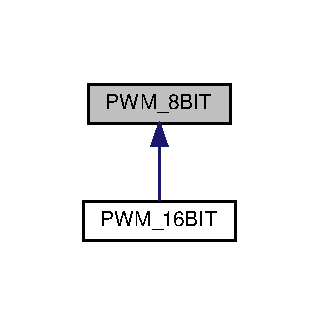
\includegraphics[width=153pt]{structPWM__8BIT__inherit__graph}
\end{center}
\end{figure}
\subsection*{Public Attributes}
\begin{DoxyCompactItemize}
\item 
\mbox{\Hypertarget{structPWM__8BIT_a67a66abe93d97084f94c41c4bb4264b7}\label{structPWM__8BIT_a67a66abe93d97084f94c41c4bb4264b7}} 
volatile uint8\+\_\+t $\ast$ {\bfseries T\+C\+C\+RxA} = (volatile uint8\+\_\+t $\ast$)0x\+FF
\item 
\mbox{\Hypertarget{structPWM__8BIT_a9b5a0f38311b0914a5011204a0039255}\label{structPWM__8BIT_a9b5a0f38311b0914a5011204a0039255}} 
volatile uint8\+\_\+t $\ast$ {\bfseries T\+C\+C\+RxB} = (volatile uint8\+\_\+t $\ast$)0x\+FF
\item 
\mbox{\Hypertarget{structPWM__8BIT_ad1f2062ca0b4dce0decf2282f045f56e}\label{structPWM__8BIT_ad1f2062ca0b4dce0decf2282f045f56e}} 
volatile uint8\+\_\+t $\ast$ {\bfseries T\+C\+N\+Tx} = (volatile uint8\+\_\+t $\ast$)0x\+FF
\item 
\mbox{\Hypertarget{structPWM__8BIT_aac6d531b2442f9217341d7c1e27aa54d}\label{structPWM__8BIT_aac6d531b2442f9217341d7c1e27aa54d}} 
volatile uint8\+\_\+t $\ast$ {\bfseries O\+C\+Rx} = (volatile uint8\+\_\+t $\ast$)0x\+FF
\end{DoxyCompactItemize}


\subsection{Detailed Description}
The \hyperlink{structPWM__8BIT}{P\+W\+M\+\_\+8\+B\+IT} struct. 

The documentation for this struct was generated from the following file\+:\begin{DoxyCompactItemize}
\item 
\hyperlink{portmanager_8h}{portmanager.\+h}\end{DoxyCompactItemize}

\hypertarget{classRdm6300}{}\section{Rdm6300 Class Reference}
\label{classRdm6300}\index{Rdm6300@{Rdm6300}}


Collaboration diagram for Rdm6300\+:\nopagebreak
\begin{figure}[H]
\begin{center}
\leavevmode
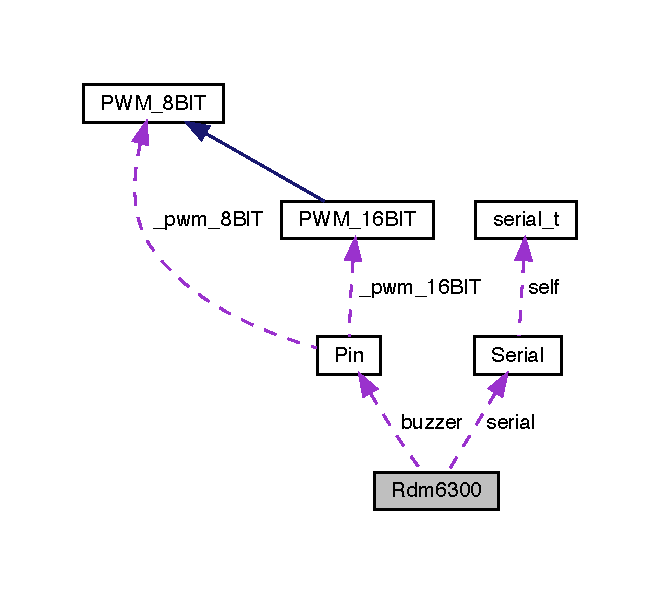
\includegraphics[width=317pt]{classRdm6300__coll__graph}
\end{center}
\end{figure}
\subsection*{Public Member Functions}
\begin{DoxyCompactItemize}
\item 
\mbox{\Hypertarget{classRdm6300_aff170c6261d9e9364d3592dea5743671}\label{classRdm6300_aff170c6261d9e9364d3592dea5743671}} 
bool {\bfseries attach\+To} (enum Serial\+Port serial, enum U\+A\+RT baud)
\item 
\mbox{\Hypertarget{classRdm6300_a09b6928f381395bf097db97bab27639d}\label{classRdm6300_a09b6928f381395bf097db97bab27639d}} 
bool {\bfseries is\+New\+Card} ()
\item 
\mbox{\Hypertarget{classRdm6300_a26db1ddb2e181b75063681a930ae296a}\label{classRdm6300_a26db1ddb2e181b75063681a930ae296a}} 
std\+::vector$<$ uint8\+\_\+t $>$ {\bfseries get\+Data} ()
\item 
\mbox{\Hypertarget{classRdm6300_ae1b10584606691ff109c5395432e7ef9}\label{classRdm6300_ae1b10584606691ff109c5395432e7ef9}} 
bool {\bfseries set\+Buzzer\+Pin} (uint8\+\_\+t pin)
\end{DoxyCompactItemize}
\subsection*{Private Member Functions}
\begin{DoxyCompactItemize}
\item 
\mbox{\Hypertarget{classRdm6300_a5a57029ca033dfb57dacb8af1279a63c}\label{classRdm6300_a5a57029ca033dfb57dacb8af1279a63c}} 
bool {\bfseries calc\+Crc} (std\+::vector$<$ uint8\+\_\+t $>$ \&buff)
\item 
\mbox{\Hypertarget{classRdm6300_a11bf89a8c306cdf0c329eb535d20c154}\label{classRdm6300_a11bf89a8c306cdf0c329eb535d20c154}} 
bool {\bfseries is\+Valid\+Packet} (std\+::vector$<$ uint8\+\_\+t $>$ \&data)
\item 
\mbox{\Hypertarget{classRdm6300_a38956667d6cd8aa2746bcdbe8de77e0c}\label{classRdm6300_a38956667d6cd8aa2746bcdbe8de77e0c}} 
void {\bfseries buzzer\+Incoming} ()
\item 
\mbox{\Hypertarget{classRdm6300_a81a9625c32a797937fecfee9268ac79d}\label{classRdm6300_a81a9625c32a797937fecfee9268ac79d}} 
void {\bfseries buzzer\+Outcoming} ()
\item 
\mbox{\Hypertarget{classRdm6300_a067a47af67954c2e845743ea5de3ebb0}\label{classRdm6300_a067a47af67954c2e845743ea5de3ebb0}} 
void {\bfseries buzzer\+Denied} ()
\end{DoxyCompactItemize}
\subsection*{Private Attributes}
\begin{DoxyCompactItemize}
\item 
\mbox{\Hypertarget{classRdm6300_aab29f639a26cfce2ef7865f829efc1d4}\label{classRdm6300_aab29f639a26cfce2ef7865f829efc1d4}} 
\mbox{\hyperlink{classSerial}{Serial}} $\ast$ {\bfseries serial}
\item 
\mbox{\Hypertarget{classRdm6300_ab67e1bc66505b024850419b28cb44371}\label{classRdm6300_ab67e1bc66505b024850419b28cb44371}} 
std\+::vector$<$ uint8\+\_\+t $>$ {\bfseries last\+Card}
\item 
\mbox{\Hypertarget{classRdm6300_adbb47250f01692e5394006137e50a1fa}\label{classRdm6300_adbb47250f01692e5394006137e50a1fa}} 
\mbox{\hyperlink{classPin}{Pin}} $\ast$ {\bfseries buzzer}
\end{DoxyCompactItemize}


The documentation for this class was generated from the following files\+:\begin{DoxyCompactItemize}
\item 
rdm630.\+h\item 
rdm630.\+cpp\end{DoxyCompactItemize}

\hypertarget{classSerial}{}\section{Serial Class Reference}
\label{classSerial}\index{Serial@{Serial}}


Inheritance diagram for Serial\+:\nopagebreak
\begin{figure}[H]
\begin{center}
\leavevmode
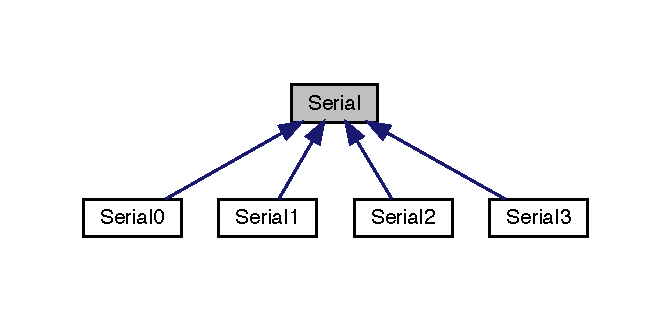
\includegraphics[width=322pt]{classSerial__inherit__graph}
\end{center}
\end{figure}


Collaboration diagram for Serial\+:\nopagebreak
\begin{figure}[H]
\begin{center}
\leavevmode
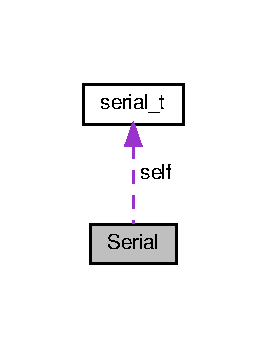
\includegraphics[width=128pt]{classSerial__coll__graph}
\end{center}
\end{figure}
\subsection*{Public Member Functions}
\begin{DoxyCompactItemize}
\item 
\mbox{\Hypertarget{classSerial_ab84837438196db931f7cb9f73f14a343}\label{classSerial_ab84837438196db931f7cb9f73f14a343}} 
void {\bfseries init} (\hyperlink{serial_8h_a6f88b8988ee3bab3eaaa301212c7f804}{U\+A\+RT} baud, \hyperlink{serial_8h_aa8b6628780447bd68953ca27d2f1acd8}{Serial\+Priority} priority=\+\_\+\+L\+O\+W\+\_\+\+P\+R\+I\+O\+R\+I\+TY)
\item 
\mbox{\Hypertarget{classSerial_a4c0b18b5cff99f166aed20fa8295ccf9}\label{classSerial_a4c0b18b5cff99f166aed20fa8295ccf9}} 
void {\bfseries printf} (const char $\ast$fmt,...)
\item 
\mbox{\Hypertarget{classSerial_aba74e314aa15524ce7cd49306accc666}\label{classSerial_aba74e314aa15524ce7cd49306accc666}} 
void {\bfseries read\+Until} (char $\ast$buffer, char chr)
\item 
\mbox{\Hypertarget{classSerial_a63b7abf172cad25bfc998b3b1f98310f}\label{classSerial_a63b7abf172cad25bfc998b3b1f98310f}} 
void {\bfseries flush} ()
\item 
\mbox{\Hypertarget{classSerial_aac4dc5a6eb54ac09c3813684295f00f4}\label{classSerial_aac4dc5a6eb54ac09c3813684295f00f4}} 
void {\bfseries set\+Rx\+I\+S\+R\+Call\+Back} (bool state)
\item 
\mbox{\Hypertarget{classSerial_aca6f48464bb0a4828177f0c70111a36a}\label{classSerial_aca6f48464bb0a4828177f0c70111a36a}} 
void {\bfseries set\+Echo\+Server} (bool state=false)
\item 
\mbox{\Hypertarget{classSerial_ad805c3cc6c46156d640f34eac1585d4a}\label{classSerial_ad805c3cc6c46156d640f34eac1585d4a}} 
void {\bfseries insert\+Data} (uint8\+\_\+t data)
\item 
\mbox{\Hypertarget{classSerial_a54041d1af51695205e804dfc911983da}\label{classSerial_a54041d1af51695205e804dfc911983da}} 
void {\bfseries inc\+Read\+Data} (uint8\+\_\+t value=1)
\item 
\mbox{\Hypertarget{classSerial_ab8ff24beb4593dd912b8091099a6ebd4}\label{classSerial_ab8ff24beb4593dd912b8091099a6ebd4}} 
void {\bfseries enable\+Shell} (bool value=false)
\item 
\mbox{\Hypertarget{classSerial_a2e870d7b7fcab20cc2d2fb70ad73764d}\label{classSerial_a2e870d7b7fcab20cc2d2fb70ad73764d}} 
void {\bfseries register\+Callback} (\hyperlink{serial_8h_ae45e33beead6f4d4d7ec9ce44c4bcc83}{ser\+\_\+cb\+\_\+t} $\ast$cb=nullptr)
\item 
\mbox{\Hypertarget{classSerial_a2485ab59468bc39160fa72ba9a22c784}\label{classSerial_a2485ab59468bc39160fa72ba9a22c784}} 
void {\bfseries rx\+Call\+Back} ()
\item 
\mbox{\Hypertarget{classSerial_a624ff162bdefdca9bcaedc3720137e1a}\label{classSerial_a624ff162bdefdca9bcaedc3720137e1a}} 
bool {\bfseries shell\+Is\+Enabled} ()
\item 
\mbox{\Hypertarget{classSerial_abe5d32f3ea45b75b8cf996b2054bc252}\label{classSerial_abe5d32f3ea45b75b8cf996b2054bc252}} 
bool {\bfseries buffer\+Is\+Readable} ()
\item 
\mbox{\Hypertarget{classSerial_afc5602930c046d828392eb1eea31c045}\label{classSerial_afc5602930c046d828392eb1eea31c045}} 
bool {\bfseries is\+Available} ()
\item 
\mbox{\Hypertarget{classSerial_add2575d5d0352d7dbb4d5aff0c08df7e}\label{classSerial_add2575d5d0352d7dbb4d5aff0c08df7e}} 
bool {\bfseries echo\+Is\+Enabled} ()
\item 
\mbox{\Hypertarget{classSerial_a2acff37fe9102262032a3f8767204c52}\label{classSerial_a2acff37fe9102262032a3f8767204c52}} 
uint8\+\_\+t {\bfseries receive} ()
\item 
\mbox{\Hypertarget{classSerial_a6453a654842a1b901bef5b789c38de65}\label{classSerial_a6453a654842a1b901bef5b789c38de65}} 
uint8\+\_\+t {\bfseries read\+Data} ()
\item 
\mbox{\Hypertarget{classSerial_a4deaf90a27cb5d2d146ee7636ed1d025}\label{classSerial_a4deaf90a27cb5d2d146ee7636ed1d025}} 
\hyperlink{serial_8h_aa8b6628780447bd68953ca27d2f1acd8}{Serial\+Priority} {\bfseries get\+Priority} ()
\item 
\mbox{\Hypertarget{classSerial_a5348fa97c36cc7f5444252d952cbedde}\label{classSerial_a5348fa97c36cc7f5444252d952cbedde}} 
void {\bfseries clear} ()
\end{DoxyCompactItemize}
\subsection*{Public Attributes}
\begin{DoxyCompactItemize}
\item 
\mbox{\Hypertarget{classSerial_a090daed60c890a076321d6bcd1c3ef0f}\label{classSerial_a090daed60c890a076321d6bcd1c3ef0f}} 
uint8\+\_\+t {\bfseries U\+S\+A\+R\+T\+\_\+\+B\+U\+FF} \mbox{[}M\+A\+X\+\_\+\+S\+E\+R\+I\+A\+L\+\_\+\+B\+U\+F\+F\+ER\mbox{]}
\end{DoxyCompactItemize}
\subsection*{Protected Member Functions}
\begin{DoxyCompactItemize}
\item 
\mbox{\Hypertarget{classSerial_a89295653be64224bbe1a11b572d9b0e4}\label{classSerial_a89295653be64224bbe1a11b572d9b0e4}} 
void {\bfseries print} (const char $\ast$str)
\end{DoxyCompactItemize}
\subsection*{Protected Attributes}
\begin{DoxyCompactItemize}
\item 
\mbox{\Hypertarget{classSerial_a71585071c3169b915300f84557d273d3}\label{classSerial_a71585071c3169b915300f84557d273d3}} 
bool {\bfseries echo\+Server}
\item 
\mbox{\Hypertarget{classSerial_a3ae40010a266baadc7a7d1c655d0f3ab}\label{classSerial_a3ae40010a266baadc7a7d1c655d0f3ab}} 
bool {\bfseries shell\+Enabled}
\item 
\mbox{\Hypertarget{classSerial_a58f8acbb0746b9dce8992d68ab380098}\label{classSerial_a58f8acbb0746b9dce8992d68ab380098}} 
bool {\bfseries buffer\+Readable}
\item 
\mbox{\Hypertarget{classSerial_a461b01260601124608caefb58aa97321}\label{classSerial_a461b01260601124608caefb58aa97321}} 
uint8\+\_\+t $\ast$ {\bfseries \+\_\+read}
\item 
\mbox{\Hypertarget{classSerial_adf357435a54ad0273470165af0b32b40}\label{classSerial_adf357435a54ad0273470165af0b32b40}} 
uint8\+\_\+t $\ast$ {\bfseries \+\_\+write}
\item 
\mbox{\Hypertarget{classSerial_ace848b00193579670c9092e2866b04c5}\label{classSerial_ace848b00193579670c9092e2866b04c5}} 
\hyperlink{structserial__t}{serial\+\_\+t} {\bfseries self}
\item 
\mbox{\Hypertarget{classSerial_a456da36721b84dab734da1b47e39545e}\label{classSerial_a456da36721b84dab734da1b47e39545e}} 
\hyperlink{serial_8h_aa8b6628780447bd68953ca27d2f1acd8}{Serial\+Priority} {\bfseries priority}
\item 
\mbox{\Hypertarget{classSerial_aa18535152da1ad701fc2470451974c32}\label{classSerial_aa18535152da1ad701fc2470451974c32}} 
\hyperlink{serial_8h_ae45e33beead6f4d4d7ec9ce44c4bcc83}{ser\+\_\+cb\+\_\+t} $\ast$ {\bfseries callback}
\end{DoxyCompactItemize}


The documentation for this class was generated from the following files\+:\begin{DoxyCompactItemize}
\item 
\hyperlink{serial_8h}{serial.\+h}\item 
serial.\+cpp\end{DoxyCompactItemize}

\hypertarget{classSerial0}{}\section{Serial0 Class Reference}
\label{classSerial0}\index{Serial0@{Serial0}}


Inheritance diagram for Serial0\+:\nopagebreak
\begin{figure}[H]
\begin{center}
\leavevmode
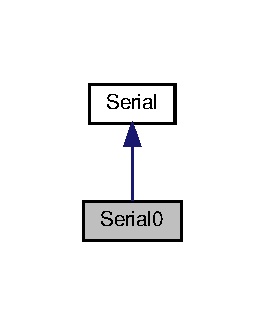
\includegraphics[width=127pt]{classSerial0__inherit__graph}
\end{center}
\end{figure}


Collaboration diagram for Serial0\+:\nopagebreak
\begin{figure}[H]
\begin{center}
\leavevmode
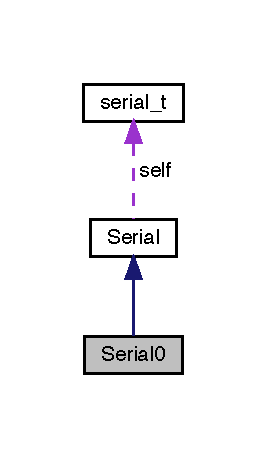
\includegraphics[width=128pt]{classSerial0__coll__graph}
\end{center}
\end{figure}
\subsection*{Friends}
\begin{DoxyCompactItemize}
\item 
\mbox{\Hypertarget{classSerial0_ae711712f6bc003a5d1156a409a19941b}\label{classSerial0_ae711712f6bc003a5d1156a409a19941b}} 
class {\bfseries Serial\+Manager}
\end{DoxyCompactItemize}
\subsection*{Additional Inherited Members}


The documentation for this class was generated from the following file\+:\begin{DoxyCompactItemize}
\item 
serial.\+h\end{DoxyCompactItemize}

\hypertarget{classSerial1}{}\section{Serial1 Class Reference}
\label{classSerial1}\index{Serial1@{Serial1}}


Inheritance diagram for Serial1\+:\nopagebreak
\begin{figure}[H]
\begin{center}
\leavevmode
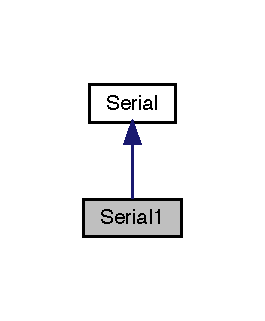
\includegraphics[width=127pt]{classSerial1__inherit__graph}
\end{center}
\end{figure}


Collaboration diagram for Serial1\+:\nopagebreak
\begin{figure}[H]
\begin{center}
\leavevmode
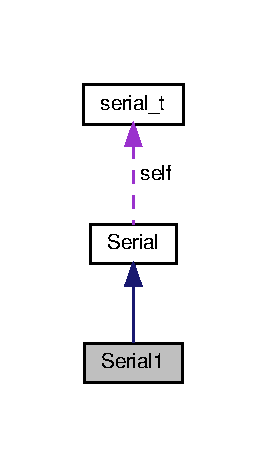
\includegraphics[width=128pt]{classSerial1__coll__graph}
\end{center}
\end{figure}
\subsection*{Friends}
\begin{DoxyCompactItemize}
\item 
\mbox{\Hypertarget{classSerial1_ae711712f6bc003a5d1156a409a19941b}\label{classSerial1_ae711712f6bc003a5d1156a409a19941b}} 
class {\bfseries Serial\+Manager}
\end{DoxyCompactItemize}
\subsection*{Additional Inherited Members}


The documentation for this class was generated from the following file\+:\begin{DoxyCompactItemize}
\item 
serial.\+h\end{DoxyCompactItemize}

\hypertarget{classSerial2}{}\section{Serial2 Class Reference}
\label{classSerial2}\index{Serial2@{Serial2}}


Inheritance diagram for Serial2\+:\nopagebreak
\begin{figure}[H]
\begin{center}
\leavevmode
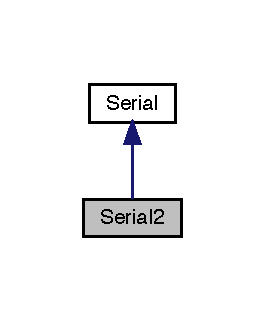
\includegraphics[width=127pt]{classSerial2__inherit__graph}
\end{center}
\end{figure}


Collaboration diagram for Serial2\+:\nopagebreak
\begin{figure}[H]
\begin{center}
\leavevmode
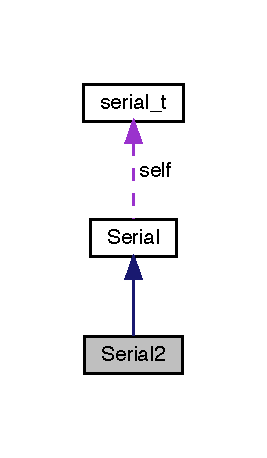
\includegraphics[width=128pt]{classSerial2__coll__graph}
\end{center}
\end{figure}
\subsection*{Friends}
\begin{DoxyCompactItemize}
\item 
\mbox{\Hypertarget{classSerial2_ae711712f6bc003a5d1156a409a19941b}\label{classSerial2_ae711712f6bc003a5d1156a409a19941b}} 
class {\bfseries Serial\+Manager}
\end{DoxyCompactItemize}
\subsection*{Additional Inherited Members}


The documentation for this class was generated from the following file\+:\begin{DoxyCompactItemize}
\item 
serial.\+h\end{DoxyCompactItemize}

\hypertarget{classSerial3}{}\section{Serial3 Class Reference}
\label{classSerial3}\index{Serial3@{Serial3}}


Inheritance diagram for Serial3\+:\nopagebreak
\begin{figure}[H]
\begin{center}
\leavevmode
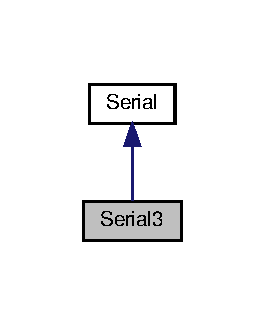
\includegraphics[width=127pt]{classSerial3__inherit__graph}
\end{center}
\end{figure}


Collaboration diagram for Serial3\+:\nopagebreak
\begin{figure}[H]
\begin{center}
\leavevmode
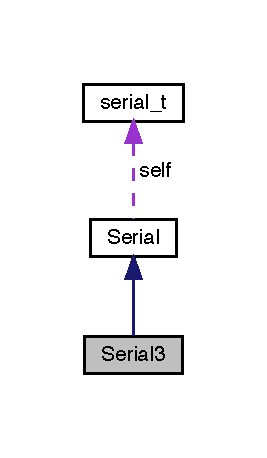
\includegraphics[width=128pt]{classSerial3__coll__graph}
\end{center}
\end{figure}
\subsection*{Friends}
\begin{DoxyCompactItemize}
\item 
\mbox{\Hypertarget{classSerial3_ae711712f6bc003a5d1156a409a19941b}\label{classSerial3_ae711712f6bc003a5d1156a409a19941b}} 
class {\bfseries Serial\+Manager}
\end{DoxyCompactItemize}
\subsection*{Additional Inherited Members}


The documentation for this class was generated from the following file\+:\begin{DoxyCompactItemize}
\item 
serial.\+h\end{DoxyCompactItemize}

\hypertarget{structserial__t}{}\section{serial\+\_\+t Struct Reference}
\label{structserial__t}\index{serial\+\_\+t@{serial\+\_\+t}}


The \hyperlink{structserial__t}{serial\+\_\+t} struct.  




{\ttfamily \#include $<$serial.\+h$>$}

\subsection*{Public Attributes}
\begin{DoxyCompactItemize}
\item 
\mbox{\Hypertarget{structserial__t_a217e81ee8801f862b447e651016bb71b}\label{structserial__t_a217e81ee8801f862b447e651016bb71b}} 
volatile uint8\+\_\+t $\ast$ {\bfseries U\+C\+S\+RxA}
\item 
\mbox{\Hypertarget{structserial__t_a2e14c00b5f729305a98f44927d91fa65}\label{structserial__t_a2e14c00b5f729305a98f44927d91fa65}} 
volatile uint8\+\_\+t $\ast$ {\bfseries U\+C\+S\+RxB}
\item 
\mbox{\Hypertarget{structserial__t_aeb6357850a478ff1c9f50f342764ed3a}\label{structserial__t_aeb6357850a478ff1c9f50f342764ed3a}} 
volatile uint8\+\_\+t $\ast$ {\bfseries U\+C\+S\+RxC}
\item 
\mbox{\Hypertarget{structserial__t_ae458e42ede033302f20deeb82d51d282}\label{structserial__t_ae458e42ede033302f20deeb82d51d282}} 
volatile uint8\+\_\+t $\ast$ {\bfseries U\+B\+R\+RxH}
\item 
\mbox{\Hypertarget{structserial__t_a9f1c7df5c88c819e1b858fede2735e82}\label{structserial__t_a9f1c7df5c88c819e1b858fede2735e82}} 
volatile uint8\+\_\+t $\ast$ {\bfseries U\+B\+R\+RxL}
\item 
\mbox{\Hypertarget{structserial__t_a4bdffabefd1f4ca2c15c249ff6300510}\label{structserial__t_a4bdffabefd1f4ca2c15c249ff6300510}} 
volatile uint8\+\_\+t $\ast$ {\bfseries U\+D\+Rx}
\end{DoxyCompactItemize}


\subsection{Detailed Description}
The \hyperlink{structserial__t}{serial\+\_\+t} struct. 

The documentation for this struct was generated from the following file\+:\begin{DoxyCompactItemize}
\item 
\hyperlink{serial_8h}{serial.\+h}\end{DoxyCompactItemize}

\hypertarget{classSerialManager}{}\section{Serial\+Manager Class Reference}
\label{classSerialManager}\index{SerialManager@{SerialManager}}
\subsection*{Static Public Member Functions}
\begin{DoxyCompactItemize}
\item 
\mbox{\Hypertarget{classSerialManager_a6b9c81d22a14b2c3a072a4c2120e5ae7}\label{classSerialManager_a6b9c81d22a14b2c3a072a4c2120e5ae7}} 
static \mbox{\hyperlink{classSerial}{Serial}} $\ast$ {\bfseries get\+Instance} (Serial\+Port port)
\end{DoxyCompactItemize}


The documentation for this class was generated from the following file\+:\begin{DoxyCompactItemize}
\item 
serial.\+h\end{DoxyCompactItemize}

\hypertarget{structslave__t}{}\section{slave\+\_\+t Struct Reference}
\label{structslave__t}\index{slave\+\_\+t@{slave\+\_\+t}}
\subsection*{Public Member Functions}
\begin{DoxyCompactItemize}
\item 
\mbox{\Hypertarget{structslave__t_a50d44b07fa05774c4c213fc5d1507227}\label{structslave__t_a50d44b07fa05774c4c213fc5d1507227}} 
{\bfseries slave\+\_\+t} (uint8\+\_\+t w\+Addr=0, uint8\+\_\+t r\+Addr=0)
\end{DoxyCompactItemize}
\subsection*{Public Attributes}
\begin{DoxyCompactItemize}
\item 
\mbox{\Hypertarget{structslave__t_a196e25cee6c8b9b6d8f66cfcba13feff}\label{structslave__t_a196e25cee6c8b9b6d8f66cfcba13feff}} 
uint8\+\_\+t {\bfseries write\+Addr}
\item 
\mbox{\Hypertarget{structslave__t_a014945119b5636f2aa55604e1b63c3d2}\label{structslave__t_a014945119b5636f2aa55604e1b63c3d2}} 
uint8\+\_\+t {\bfseries read\+Addr}
\end{DoxyCompactItemize}


The documentation for this struct was generated from the following file\+:\begin{DoxyCompactItemize}
\item 
i2cmaster.\+h\end{DoxyCompactItemize}

\hypertarget{classSlaveSPI}{}\section{Slave\+S\+PI Class Reference}
\label{classSlaveSPI}\index{Slave\+S\+PI@{Slave\+S\+PI}}


Collaboration diagram for Slave\+S\+PI\+:\nopagebreak
\begin{figure}[H]
\begin{center}
\leavevmode
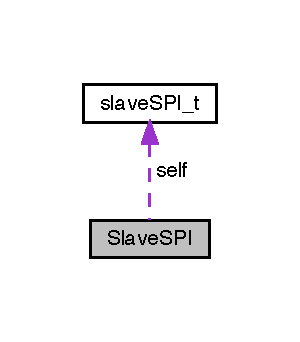
\includegraphics[width=144pt]{classSlaveSPI__coll__graph}
\end{center}
\end{figure}
\subsection*{Public Member Functions}
\begin{DoxyCompactItemize}
\item 
\mbox{\Hypertarget{classSlaveSPI_a1a89540f74f13d1189540158df8cdcc0}\label{classSlaveSPI_a1a89540f74f13d1189540158df8cdcc0}} 
void {\bfseries set\+I\+SR} (bool value=false)
\item 
\mbox{\Hypertarget{classSlaveSPI_a285c49176f81546e1d50858a9fb4b679}\label{classSlaveSPI_a285c49176f81546e1d50858a9fb4b679}} 
void {\bfseries send} (uint8\+\_\+t data)
\item 
\mbox{\Hypertarget{classSlaveSPI_a20e086294af941e947ad28bc2632b0e5}\label{classSlaveSPI_a20e086294af941e947ad28bc2632b0e5}} 
void {\bfseries send} (uint8\+\_\+t $\ast$buff, size\+\_\+t size)
\item 
\mbox{\Hypertarget{classSlaveSPI_a10b62b984e18c7488f3a441bf81726a4}\label{classSlaveSPI_a10b62b984e18c7488f3a441bf81726a4}} 
uint8\+\_\+t {\bfseries receive} ()
\item 
\mbox{\Hypertarget{classSlaveSPI_a47a1a8f35c4386d72e29b6850c6b9519}\label{classSlaveSPI_a47a1a8f35c4386d72e29b6850c6b9519}} 
void {\bfseries receive} (uint8\+\_\+t $\ast$buff, size\+\_\+t size)
\item 
\mbox{\Hypertarget{classSlaveSPI_a4e488538a3ba502d7e81a0380e012986}\label{classSlaveSPI_a4e488538a3ba502d7e81a0380e012986}} 
bool {\bfseries bus\+Is\+Writable} ()
\item 
\mbox{\Hypertarget{classSlaveSPI_a6dc365f65961de53d09d3ed8243a48c8}\label{classSlaveSPI_a6dc365f65961de53d09d3ed8243a48c8}} 
void {\bfseries register\+Callback} (spi\+\_\+cb\+\_\+t $\ast$cb)
\item 
\mbox{\Hypertarget{classSlaveSPI_afd171add4870a19ec6eb9fa63c479de3}\label{classSlaveSPI_afd171add4870a19ec6eb9fa63c479de3}} 
void {\bfseries callback} (uint8\+\_\+t data)
\item 
\mbox{\Hypertarget{classSlaveSPI_a8f0330b4050492a51e2d359a980734d0}\label{classSlaveSPI_a8f0330b4050492a51e2d359a980734d0}} 
void {\bfseries insert\+Data} (uint8\+\_\+t data)
\item 
\mbox{\Hypertarget{classSlaveSPI_aa89118ab2eda4f4e31617b3590568706}\label{classSlaveSPI_aa89118ab2eda4f4e31617b3590568706}} 
uint8\+\_\+t {\bfseries read\+Data} ()
\item 
\mbox{\Hypertarget{classSlaveSPI_a29b4bec6bb4e7aa3082aeeec5d37ea4f}\label{classSlaveSPI_a29b4bec6bb4e7aa3082aeeec5d37ea4f}} 
bool {\bfseries buffer\+Is\+Readable} ()
\end{DoxyCompactItemize}
\subsection*{Static Public Member Functions}
\begin{DoxyCompactItemize}
\item 
\mbox{\Hypertarget{classSlaveSPI_af853e49df2daa8df562c211d4c01c825}\label{classSlaveSPI_af853e49df2daa8df562c211d4c01c825}} 
static \hyperlink{classSlaveSPI}{Slave\+S\+PI} $\ast$ {\bfseries get\+Instance} (\hyperlink{structslaveSPI__t}{slave\+S\+P\+I\+\_\+t} data=nullptr)
\end{DoxyCompactItemize}
\subsection*{Private Member Functions}
\begin{DoxyCompactItemize}
\item 
\mbox{\Hypertarget{classSlaveSPI_a4e4d482325a3cdd0f626130ba351c402}\label{classSlaveSPI_a4e4d482325a3cdd0f626130ba351c402}} 
{\bfseries Slave\+S\+PI} (\hyperlink{structslaveSPI__t}{slave\+S\+P\+I\+\_\+t} data, S\+P\+I\+\_\+\+D\+O\+RD data\+Order=M\+S\+B\+\_\+\+F\+I\+R\+ST, S\+P\+I\+\_\+\+C\+L\+K\+S\+EL clock\+Sel=F\+O\+S\+C\+\_\+\+B\+Y\+\_\+2, S\+P\+I\+\_\+\+C\+P\+OL clock\+Polarity=L\+R\+\_\+\+TF, S\+P\+I\+\_\+\+C\+P\+HA clock\+Phase=L\+S\+\_\+\+TP)
\end{DoxyCompactItemize}
\subsection*{Private Attributes}
\begin{DoxyCompactItemize}
\item 
\mbox{\Hypertarget{classSlaveSPI_a6a33cdba141195a5a8157aed8dd39527}\label{classSlaveSPI_a6a33cdba141195a5a8157aed8dd39527}} 
uint8\+\_\+t {\bfseries S\+P\+I\+\_\+\+B\+U\+FF} \mbox{[}M\+A\+X\+\_\+\+S\+P\+I\+\_\+\+B\+U\+F\+F\+ER\mbox{]}
\item 
\mbox{\Hypertarget{classSlaveSPI_a4c6a1758bdfcc6b7987aa8aaade47e57}\label{classSlaveSPI_a4c6a1758bdfcc6b7987aa8aaade47e57}} 
\hyperlink{structslaveSPI__t}{slave\+S\+P\+I\+\_\+t} {\bfseries self}
\item 
\mbox{\Hypertarget{classSlaveSPI_adaf64cc08db2c73c7304d1ab9e6ef7c4}\label{classSlaveSPI_adaf64cc08db2c73c7304d1ab9e6ef7c4}} 
spi\+\_\+cb\+\_\+t $\ast$ {\bfseries \+\_\+callback}
\item 
\mbox{\Hypertarget{classSlaveSPI_ad9cf150323ece7a6f842d678b2aa1b79}\label{classSlaveSPI_ad9cf150323ece7a6f842d678b2aa1b79}} 
uint8\+\_\+t $\ast$ {\bfseries \+\_\+read}
\item 
\mbox{\Hypertarget{classSlaveSPI_a7ce2f27aafe7c97bf92426aa79d7c4cf}\label{classSlaveSPI_a7ce2f27aafe7c97bf92426aa79d7c4cf}} 
uint8\+\_\+t $\ast$ {\bfseries \+\_\+write}
\item 
\mbox{\Hypertarget{classSlaveSPI_ab4d9e7eebaaead1f8dde9f933bfec2f1}\label{classSlaveSPI_ab4d9e7eebaaead1f8dde9f933bfec2f1}} 
bool {\bfseries buffer\+Readable}
\end{DoxyCompactItemize}


The documentation for this class was generated from the following files\+:\begin{DoxyCompactItemize}
\item 
\hyperlink{spislave_8h}{spislave.\+h}\item 
spislave.\+cpp\end{DoxyCompactItemize}

\hypertarget{structslaveSPI__t}{}\section{slave\+S\+P\+I\+\_\+t Struct Reference}
\label{structslaveSPI__t}\index{slaveSPI\_t@{slaveSPI\_t}}
\subsection*{Public Member Functions}
\begin{DoxyCompactItemize}
\item 
\mbox{\Hypertarget{structslaveSPI__t_a1b6a92bfd0ff9f66643a2216703070fe}\label{structslaveSPI__t_a1b6a92bfd0ff9f66643a2216703070fe}} 
{\bfseries slave\+S\+P\+I\+\_\+t} (volatile uint8\+\_\+t $\ast$pinx=nullptr, \mbox{\hyperlink{classPin}{Pin}} $\ast$miso=nullptr, \mbox{\hyperlink{classPin}{Pin}} $\ast$mosi=nullptr, \mbox{\hyperlink{classPin}{Pin}} $\ast$sck=nullptr, \mbox{\hyperlink{classPin}{Pin}} $\ast$ss=nullptr)
\end{DoxyCompactItemize}
\subsection*{Public Attributes}
\begin{DoxyCompactItemize}
\item 
\mbox{\Hypertarget{structslaveSPI__t_a87109c268334437e6c10cde1a0ba03af}\label{structslaveSPI__t_a87109c268334437e6c10cde1a0ba03af}} 
volatile uint8\+\_\+t $\ast$ {\bfseries P\+I\+Nx}
\item 
\mbox{\Hypertarget{structslaveSPI__t_a77665ecee539253948fc71839bc554e7}\label{structslaveSPI__t_a77665ecee539253948fc71839bc554e7}} 
volatile uint8\+\_\+t $\ast$ {\bfseries D\+D\+Rx}
\item 
\mbox{\Hypertarget{structslaveSPI__t_a5588c63730f0f979979505bc9fd9c549}\label{structslaveSPI__t_a5588c63730f0f979979505bc9fd9c549}} 
volatile uint8\+\_\+t $\ast$ {\bfseries P\+O\+R\+Tx}
\item 
\mbox{\Hypertarget{structslaveSPI__t_ad9840e1a743e4e44ceb98423dbf9e187}\label{structslaveSPI__t_ad9840e1a743e4e44ceb98423dbf9e187}} 
uint8\+\_\+t {\bfseries M\+I\+SO}
\item 
\mbox{\Hypertarget{structslaveSPI__t_afa1934adc11d621b99622b2c3d64f39c}\label{structslaveSPI__t_afa1934adc11d621b99622b2c3d64f39c}} 
uint8\+\_\+t {\bfseries M\+O\+SI}
\item 
\mbox{\Hypertarget{structslaveSPI__t_a9806668f14328150edfee7d9c9c50c16}\label{structslaveSPI__t_a9806668f14328150edfee7d9c9c50c16}} 
uint8\+\_\+t {\bfseries S\+CK}
\item 
\mbox{\Hypertarget{structslaveSPI__t_a784ce6629767e64b0bbe7ffcf2937d52}\label{structslaveSPI__t_a784ce6629767e64b0bbe7ffcf2937d52}} 
uint8\+\_\+t {\bfseries SS}
\end{DoxyCompactItemize}


The documentation for this struct was generated from the following file\+:\begin{DoxyCompactItemize}
\item 
spislave.\+h\end{DoxyCompactItemize}

\hypertarget{classTcp}{}\section{Tcp Class Reference}
\label{classTcp}\index{Tcp@{Tcp}}


Collaboration diagram for Tcp\+:\nopagebreak
\begin{figure}[H]
\begin{center}
\leavevmode
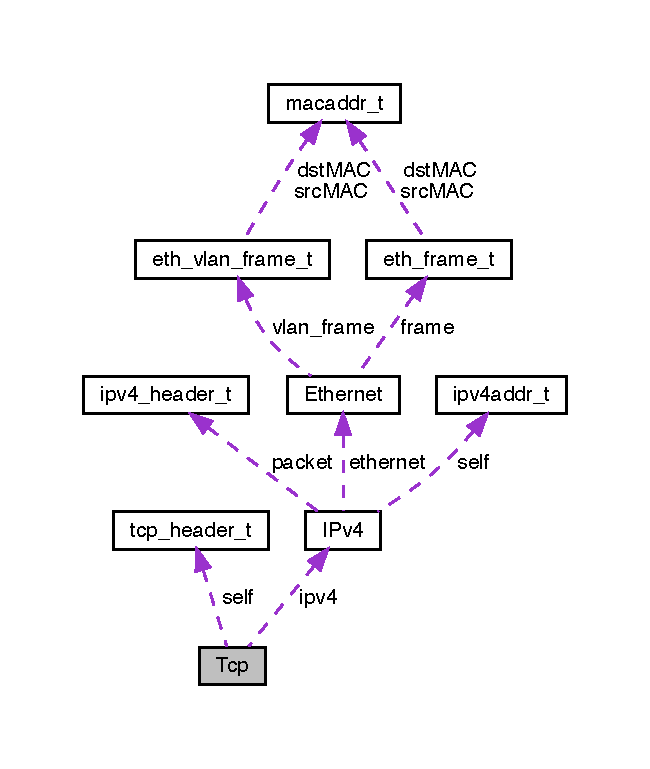
\includegraphics[width=309pt]{classTcp__coll__graph}
\end{center}
\end{figure}
\subsection*{Public Member Functions}
\begin{DoxyCompactItemize}
\item 
\mbox{\Hypertarget{classTcp_aff0ea81b11c297e17b8791a0c03a8589}\label{classTcp_aff0ea81b11c297e17b8791a0c03a8589}} 
void {\bfseries encapsulate} (std\+::vector$<$ u8t $>$ \&payload)
\item 
\mbox{\Hypertarget{classTcp_ac11613828a7a445052a338e521706ffe}\label{classTcp_ac11613828a7a445052a338e521706ffe}} 
std\+::vector$<$ u8t $>$ {\bfseries decapsulate} (std\+::vector$<$ u8t $>$ \&data)
\end{DoxyCompactItemize}
\subsection*{Private Member Functions}
\begin{DoxyCompactItemize}
\item 
\mbox{\Hypertarget{classTcp_a5f8fee77a1e98bbf3e38419e14cd2b20}\label{classTcp_a5f8fee77a1e98bbf3e38419e14cd2b20}} 
u16t {\bfseries gen\+Random\+Port} ()
\end{DoxyCompactItemize}
\subsection*{Private Attributes}
\begin{DoxyCompactItemize}
\item 
\mbox{\Hypertarget{classTcp_a8d534d9756bb2da25562007ea4f7d892}\label{classTcp_a8d534d9756bb2da25562007ea4f7d892}} 
\hyperlink{structtcp__header__t}{tcp\+\_\+header\+\_\+t} {\bfseries self}
\item 
\mbox{\Hypertarget{classTcp_af11f1b485c7082948b0c97d4e1fd1fb5}\label{classTcp_af11f1b485c7082948b0c97d4e1fd1fb5}} 
\hyperlink{classIPv4}{I\+Pv4} {\bfseries ipv4}
\end{DoxyCompactItemize}


The documentation for this class was generated from the following files\+:\begin{DoxyCompactItemize}
\item 
tcp.\+h\item 
tcp.\+cpp\end{DoxyCompactItemize}

\hypertarget{structtcp__header__t}{}\section{tcp\+\_\+header\+\_\+t Struct Reference}
\label{structtcp__header__t}\index{tcp\+\_\+header\+\_\+t@{tcp\+\_\+header\+\_\+t}}
\subsection*{Public Member Functions}
\begin{DoxyCompactItemize}
\item 
\mbox{\Hypertarget{structtcp__header__t_a8059c930a72b7fa280e74c72425c4a2f}\label{structtcp__header__t_a8059c930a72b7fa280e74c72425c4a2f}} 
{\bfseries tcp\+\_\+header\+\_\+t} (\hyperlink{macros_8h_a590a9a8f7df8fabfac6573e21da1922d}{u16t} src\+Port=0, \hyperlink{macros_8h_a590a9a8f7df8fabfac6573e21da1922d}{u16t} dst\+Port=0, \hyperlink{macros_8h_a464a07ed2c6d005d677113cc44750a64}{u32t} seq\+Number=0, \hyperlink{macros_8h_a464a07ed2c6d005d677113cc44750a64}{u32t} ack\+Number=0, \hyperlink{macros_8h_a176a4ab0531a048e0693a4520c550193}{u8t} data\+Offset=0, \hyperlink{macros_8h_a176a4ab0531a048e0693a4520c550193}{u8t} E\+CN=0, \hyperlink{macros_8h_a176a4ab0531a048e0693a4520c550193}{u8t} control\+Bits=0, \hyperlink{macros_8h_a590a9a8f7df8fabfac6573e21da1922d}{u16t} window=0, \hyperlink{macros_8h_a590a9a8f7df8fabfac6573e21da1922d}{u16t} crc=0, \hyperlink{macros_8h_a590a9a8f7df8fabfac6573e21da1922d}{u16t} urgent\+Pointer=0, \hyperlink{macros_8h_a464a07ed2c6d005d677113cc44750a64}{u32t} option\+\_\+pad=0)
\end{DoxyCompactItemize}
\subsection*{Public Attributes}
\begin{DoxyCompactItemize}
\item 
\mbox{\Hypertarget{structtcp__header__t_ab17e30c5b73eda905376cffc6e96b27e}\label{structtcp__header__t_ab17e30c5b73eda905376cffc6e96b27e}} 
\hyperlink{macros_8h_a590a9a8f7df8fabfac6573e21da1922d}{u16t} {\bfseries src\+Port}
\item 
\mbox{\Hypertarget{structtcp__header__t_aa1637617627d696a0d00b7db9a0c3e05}\label{structtcp__header__t_aa1637617627d696a0d00b7db9a0c3e05}} 
\hyperlink{macros_8h_a590a9a8f7df8fabfac6573e21da1922d}{u16t} {\bfseries dst\+Port}
\item 
\mbox{\Hypertarget{structtcp__header__t_acd373805c52a50636660a35adfbd6730}\label{structtcp__header__t_acd373805c52a50636660a35adfbd6730}} 
\hyperlink{macros_8h_a464a07ed2c6d005d677113cc44750a64}{u32t} {\bfseries seq\+Number}
\item 
\mbox{\Hypertarget{structtcp__header__t_a16a113bd0f6979ce68293292cd2a9434}\label{structtcp__header__t_a16a113bd0f6979ce68293292cd2a9434}} 
\hyperlink{macros_8h_a464a07ed2c6d005d677113cc44750a64}{u32t} {\bfseries ack\+Number}
\item 
\mbox{\Hypertarget{structtcp__header__t_a85a41a2af5b99f168ab4521a19230eda}\label{structtcp__header__t_a85a41a2af5b99f168ab4521a19230eda}} 
\hyperlink{macros_8h_a176a4ab0531a048e0693a4520c550193}{u8t} {\bfseries data\+Offset}\+:4
\item 
\mbox{\Hypertarget{structtcp__header__t_a0ecad51922d8f16d7c260bc6979548d4}\label{structtcp__header__t_a0ecad51922d8f16d7c260bc6979548d4}} 
\hyperlink{macros_8h_a176a4ab0531a048e0693a4520c550193}{u8t} {\bfseries reserved}\+:3
\item 
\mbox{\Hypertarget{structtcp__header__t_a93d31f86f389129044eb25ddf8d6c776}\label{structtcp__header__t_a93d31f86f389129044eb25ddf8d6c776}} 
\hyperlink{macros_8h_a176a4ab0531a048e0693a4520c550193}{u8t} {\bfseries E\+CN}\+:3
\item 
\mbox{\Hypertarget{structtcp__header__t_a68fe920f9ea75e505ffaae2c2f459643}\label{structtcp__header__t_a68fe920f9ea75e505ffaae2c2f459643}} 
\hyperlink{macros_8h_a176a4ab0531a048e0693a4520c550193}{u8t} {\bfseries control\+Bits}\+:6
\item 
\mbox{\Hypertarget{structtcp__header__t_a3dab5b7dabccaad92e62208b4bea4f31}\label{structtcp__header__t_a3dab5b7dabccaad92e62208b4bea4f31}} 
\hyperlink{macros_8h_a590a9a8f7df8fabfac6573e21da1922d}{u16t} {\bfseries window}
\item 
\mbox{\Hypertarget{structtcp__header__t_a77f30d1156bb756a032d22ddf7da68be}\label{structtcp__header__t_a77f30d1156bb756a032d22ddf7da68be}} 
\hyperlink{macros_8h_a590a9a8f7df8fabfac6573e21da1922d}{u16t} {\bfseries crc}
\item 
\mbox{\Hypertarget{structtcp__header__t_a276b80e1695467a2e1e0042e2007bb6e}\label{structtcp__header__t_a276b80e1695467a2e1e0042e2007bb6e}} 
\hyperlink{macros_8h_a590a9a8f7df8fabfac6573e21da1922d}{u16t} {\bfseries urgent\+Pointer}
\item 
\mbox{\Hypertarget{structtcp__header__t_aa0942cb51895cd56edbf6e7c38ac001c}\label{structtcp__header__t_aa0942cb51895cd56edbf6e7c38ac001c}} 
\hyperlink{macros_8h_a464a07ed2c6d005d677113cc44750a64}{u32t} {\bfseries option\+\_\+pad}
\item 
\mbox{\Hypertarget{structtcp__header__t_a21fd2ea47b4350e682d309ce6aa8c311}\label{structtcp__header__t_a21fd2ea47b4350e682d309ce6aa8c311}} 
std\+::vector$<$ \hyperlink{macros_8h_a176a4ab0531a048e0693a4520c550193}{u8t} $>$ {\bfseries payload}
\end{DoxyCompactItemize}


The documentation for this struct was generated from the following file\+:\begin{DoxyCompactItemize}
\item 
tcp.\+h\end{DoxyCompactItemize}

\hypertarget{structTime}{}\section{Time Struct Reference}
\label{structTime}\index{Time@{Time}}
\subsection*{Public Attributes}
\begin{DoxyCompactItemize}
\item 
\mbox{\Hypertarget{structTime_aad746065c17bb222dc72c4112828a8f6}\label{structTime_aad746065c17bb222dc72c4112828a8f6}} 
uint32\+\_\+t {\bfseries micro\+Seconds}
\end{DoxyCompactItemize}


The documentation for this struct was generated from the following file\+:\begin{DoxyCompactItemize}
\item 
timer.\+h\end{DoxyCompactItemize}

\hypertarget{classTimer}{}\section{Timer Class Reference}
\label{classTimer}\index{Timer@{Timer}}


Collaboration diagram for Timer\+:\nopagebreak
\begin{figure}[H]
\begin{center}
\leavevmode
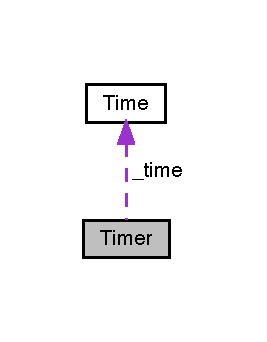
\includegraphics[width=128pt]{classTimer__coll__graph}
\end{center}
\end{figure}
\subsection*{Static Public Member Functions}
\begin{DoxyCompactItemize}
\item 
\mbox{\Hypertarget{classTimer_a00eca12a53538b339a927723a246e2d7}\label{classTimer_a00eca12a53538b339a927723a246e2d7}} 
static void {\bfseries init} ()
\item 
\mbox{\Hypertarget{classTimer_a3a8b5272198d029779dc9302a54305a8}\label{classTimer_a3a8b5272198d029779dc9302a54305a8}} 
static void {\bfseries start} ()
\item 
\mbox{\Hypertarget{classTimer_a63f0eb44b27402196590a03781515dba}\label{classTimer_a63f0eb44b27402196590a03781515dba}} 
static void {\bfseries stop} ()
\item 
\mbox{\Hypertarget{classTimer_a8b32de7275bebb6ecc51385f1f1d1d43}\label{classTimer_a8b32de7275bebb6ecc51385f1f1d1d43}} 
static uint32\+\_\+t {\bfseries now} ()
\end{DoxyCompactItemize}
\subsection*{Static Public Attributes}
\begin{DoxyCompactItemize}
\item 
\mbox{\Hypertarget{classTimer_a831586e44562c0ea423344197dc8e529}\label{classTimer_a831586e44562c0ea423344197dc8e529}} 
static \hyperlink{structTime}{Time} {\bfseries \+\_\+time}
\end{DoxyCompactItemize}
\subsection*{Static Private Attributes}
\begin{DoxyCompactItemize}
\item 
\mbox{\Hypertarget{classTimer_a0a01a2bb877f90195f529562b5f34d9f}\label{classTimer_a0a01a2bb877f90195f529562b5f34d9f}} 
static bool {\bfseries \+\_\+is\+Init} = false
\end{DoxyCompactItemize}


The documentation for this class was generated from the following files\+:\begin{DoxyCompactItemize}
\item 
\hyperlink{timer_8h}{timer.\+h}\item 
timer.\+cpp\end{DoxyCompactItemize}

\hypertarget{classUdp}{}\section{Udp Class Reference}
\label{classUdp}\index{Udp@{Udp}}


The documentation for this class was generated from the following files\+:\begin{DoxyCompactItemize}
\item 
udp.\+h\item 
udp.\+cpp\end{DoxyCompactItemize}

\hypertarget{structudp__header__t}{}\section{udp\+\_\+header\+\_\+t Struct Reference}
\label{structudp__header__t}\index{udp\_header\_t@{udp\_header\_t}}
\subsection*{Public Attributes}
\begin{DoxyCompactItemize}
\item 
\mbox{\Hypertarget{structudp__header__t_a75c64ae2804e9f789e157e914eef7f59}\label{structudp__header__t_a75c64ae2804e9f789e157e914eef7f59}} 
u16t {\bfseries src\+Port}
\item 
\mbox{\Hypertarget{structudp__header__t_a2bd45c541cea7ceba3a45dd50c06f6a3}\label{structudp__header__t_a2bd45c541cea7ceba3a45dd50c06f6a3}} 
u16t {\bfseries dst\+Port}
\item 
\mbox{\Hypertarget{structudp__header__t_a2525804fef03fb73295d27ee6ada737b}\label{structudp__header__t_a2525804fef03fb73295d27ee6ada737b}} 
u16t {\bfseries length}
\item 
\mbox{\Hypertarget{structudp__header__t_a60927678afdb28e824ce916f8299bd01}\label{structudp__header__t_a60927678afdb28e824ce916f8299bd01}} 
u16t {\bfseries crc}
\end{DoxyCompactItemize}


The documentation for this struct was generated from the following file\+:\begin{DoxyCompactItemize}
\item 
udp.\+h\end{DoxyCompactItemize}

\hypertarget{classyanujz_1_1vector}{}\section{yanujz\+::vector$<$ T $>$ Class Template Reference}
\label{classyanujz_1_1vector}\index{yanujz::vector$<$ T $>$@{yanujz::vector$<$ T $>$}}
\subsection*{Public Member Functions}
\begin{DoxyCompactItemize}
\item 
\mbox{\Hypertarget{classyanujz_1_1vector_afc2995df62370c8bffab0952d82e69d1}\label{classyanujz_1_1vector_afc2995df62370c8bffab0952d82e69d1}} 
{\bfseries vector} (T $\ast$ptr, size\+\_\+t size)
\item 
\mbox{\Hypertarget{classyanujz_1_1vector_a4f73ceed1f2fab819718827b77240b31}\label{classyanujz_1_1vector_a4f73ceed1f2fab819718827b77240b31}} 
T {\bfseries get\+Value} (T index)
\item 
\mbox{\Hypertarget{classyanujz_1_1vector_aaecd4b3fb974c266c26cc1ff56b4f9b7}\label{classyanujz_1_1vector_aaecd4b3fb974c266c26cc1ff56b4f9b7}} 
T {\bfseries first} ()
\item 
\mbox{\Hypertarget{classyanujz_1_1vector_ab87af80e5f0ab58ae0a980f9a71535bc}\label{classyanujz_1_1vector_ab87af80e5f0ab58ae0a980f9a71535bc}} 
T {\bfseries last} ()
\item 
\mbox{\Hypertarget{classyanujz_1_1vector_a8e03dc943257d9aa5d8575458706d7ab}\label{classyanujz_1_1vector_a8e03dc943257d9aa5d8575458706d7ab}} 
T $\ast$ {\bfseries begin} () const
\item 
\mbox{\Hypertarget{classyanujz_1_1vector_ac3ae405b734f1b27dac9262f57858fe6}\label{classyanujz_1_1vector_ac3ae405b734f1b27dac9262f57858fe6}} 
T $\ast$ {\bfseries end} () const
\item 
\mbox{\Hypertarget{classyanujz_1_1vector_a8ae16eebf17e251f68741c3bdb6194dc}\label{classyanujz_1_1vector_a8ae16eebf17e251f68741c3bdb6194dc}} 
void {\bfseries push\+Left} (T value)
\item 
\mbox{\Hypertarget{classyanujz_1_1vector_adeb4def36589813d937b60a66bbcfc12}\label{classyanujz_1_1vector_adeb4def36589813d937b60a66bbcfc12}} 
void {\bfseries push\+Left} (T arr\mbox{[}$\,$\mbox{]}, T size)
\item 
\mbox{\Hypertarget{classyanujz_1_1vector_af12781ddff0fc729f68278f76822e25e}\label{classyanujz_1_1vector_af12781ddff0fc729f68278f76822e25e}} 
void {\bfseries push\+Right} (T value)
\item 
\mbox{\Hypertarget{classyanujz_1_1vector_a10bc16f91c1d549cfb2105e4ca9f4f39}\label{classyanujz_1_1vector_a10bc16f91c1d549cfb2105e4ca9f4f39}} 
void {\bfseries insert} (size\+\_\+t index, T arr\mbox{[}$\,$\mbox{]}, size\+\_\+t size)
\item 
\mbox{\Hypertarget{classyanujz_1_1vector_a842a2fee1debbcbfc93acfe2603789f6}\label{classyanujz_1_1vector_a842a2fee1debbcbfc93acfe2603789f6}} 
void {\bfseries insert} (T $\ast$dst, T $\ast$src\+Start, T $\ast$src\+End)
\item 
\mbox{\Hypertarget{classyanujz_1_1vector_a2575a44b1ec73b0e9d733b25cc88d373}\label{classyanujz_1_1vector_a2575a44b1ec73b0e9d733b25cc88d373}} 
void {\bfseries pop\+Right} (size\+\_\+t value=1)
\item 
\mbox{\Hypertarget{classyanujz_1_1vector_a475cb1209615caeff951aaeb3054a9d9}\label{classyanujz_1_1vector_a475cb1209615caeff951aaeb3054a9d9}} 
void {\bfseries pop\+Left} (size\+\_\+t value=1)
\item 
\mbox{\Hypertarget{classyanujz_1_1vector_acadcada884c64b846e3e56920c4dbce8}\label{classyanujz_1_1vector_acadcada884c64b846e3e56920c4dbce8}} 
size\+\_\+t {\bfseries size} () const
\item 
\mbox{\Hypertarget{classyanujz_1_1vector_a972426cdc2a35b7f8eb13ad8fa39b2ce}\label{classyanujz_1_1vector_a972426cdc2a35b7f8eb13ad8fa39b2ce}} 
bool {\bfseries empty} ()
\item 
\mbox{\Hypertarget{classyanujz_1_1vector_af00bcbaec1205084ee5c62e49d7830c9}\label{classyanujz_1_1vector_af00bcbaec1205084ee5c62e49d7830c9}} 
void {\bfseries clear} ()
\item 
\mbox{\Hypertarget{classyanujz_1_1vector_aaf13006bde6bbf9e048c0d686651c799}\label{classyanujz_1_1vector_aaf13006bde6bbf9e048c0d686651c799}} 
T $\ast$ {\bfseries data} ()
\item 
\mbox{\Hypertarget{classyanujz_1_1vector_a4d96fe343042e6c536848ddd929b5bae}\label{classyanujz_1_1vector_a4d96fe343042e6c536848ddd929b5bae}} 
T {\bfseries at} (size\+\_\+t index) const
\item 
\mbox{\Hypertarget{classyanujz_1_1vector_a57bd3e4c1ce3f46a299d72ae3b72a21c}\label{classyanujz_1_1vector_a57bd3e4c1ce3f46a299d72ae3b72a21c}} 
T \& {\bfseries operator\mbox{[}$\,$\mbox{]}} (size\+\_\+t index)
\item 
\mbox{\Hypertarget{classyanujz_1_1vector_afb06d63c6b009adc19b3feffebe1a9f8}\label{classyanujz_1_1vector_afb06d63c6b009adc19b3feffebe1a9f8}} 
\mbox{\hyperlink{classyanujz_1_1vector}{vector}}$<$ T $>$ \& {\bfseries operator=} (const \mbox{\hyperlink{classyanujz_1_1vector}{vector}}$<$ T $>$ \&v)
\item 
\mbox{\Hypertarget{classyanujz_1_1vector_a12fd3f96a48429653425813feaa69b29}\label{classyanujz_1_1vector_a12fd3f96a48429653425813feaa69b29}} 
bool {\bfseries operator==} (const \mbox{\hyperlink{classyanujz_1_1vector}{vector}}$<$ T $>$ \&rhs)
\item 
\mbox{\Hypertarget{classyanujz_1_1vector_a260121ff22a82eb25d56b6ed2e9b256d}\label{classyanujz_1_1vector_a260121ff22a82eb25d56b6ed2e9b256d}} 
bool {\bfseries operator!=} (\mbox{\hyperlink{classyanujz_1_1vector}{vector}}$<$ T $>$ \&rhs)
\end{DoxyCompactItemize}
\subsection*{Private Attributes}
\begin{DoxyCompactItemize}
\item 
\mbox{\Hypertarget{classyanujz_1_1vector_a1483399bbd46921c629ec261bb8121b2}\label{classyanujz_1_1vector_a1483399bbd46921c629ec261bb8121b2}} 
T $\ast$ {\bfseries \+\_\+value}
\item 
\mbox{\Hypertarget{classyanujz_1_1vector_afffae7fe8ce95b099280e12652daf43c}\label{classyanujz_1_1vector_afffae7fe8ce95b099280e12652daf43c}} 
size\+\_\+t {\bfseries \+\_\+size}
\end{DoxyCompactItemize}


The documentation for this class was generated from the following file\+:\begin{DoxyCompactItemize}
\item 
vector.\+h\end{DoxyCompactItemize}

\chapter{File Documentation}
\hypertarget{net__utils_8h}{}\section{net\+\_\+utils.\+h File Reference}
\label{net__utils_8h}\index{net\+\_\+utils.\+h@{net\+\_\+utils.\+h}}
{\ttfamily \#include $<$macros.\+h$>$}\newline
{\ttfamily \#include $<$utils.\+h$>$}\newline
{\ttfamily \#include $<$strutil.\+h$>$}\newline
{\ttfamily \#include $<$string.\+h$>$}\newline
{\ttfamily \#include $<$stdlib.\+h$>$}\newline
{\ttfamily \#include $<$inet\+\_\+global.\+h$>$}\newline
Include dependency graph for net\+\_\+utils.\+h\+:\nopagebreak
\begin{figure}[H]
\begin{center}
\leavevmode
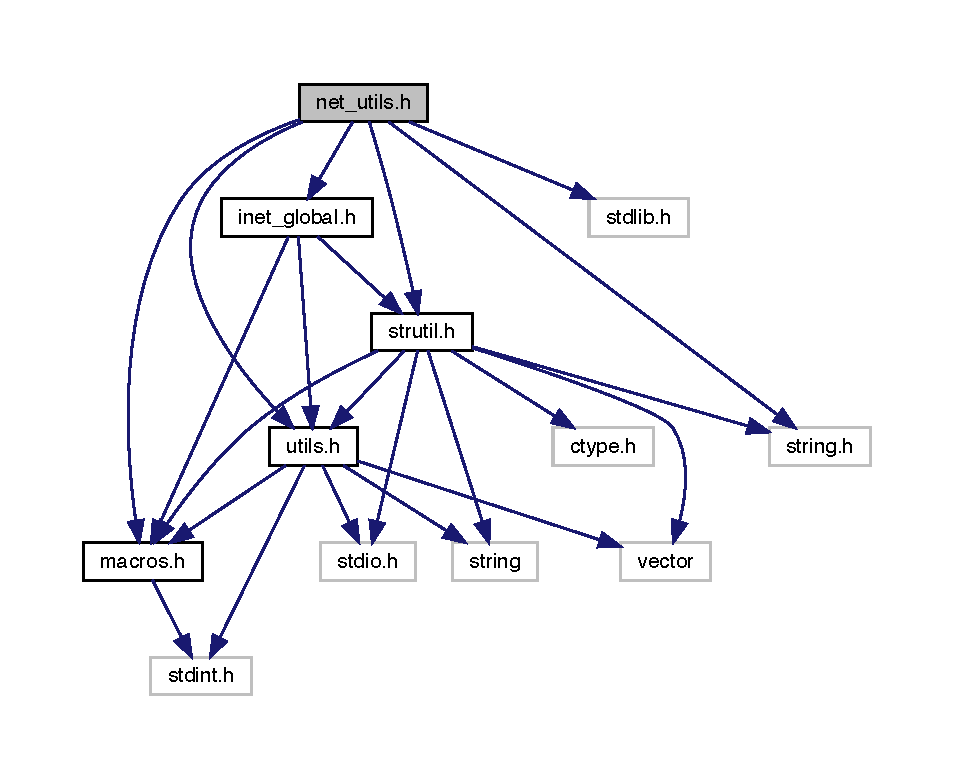
\includegraphics[width=350pt]{net__utils_8h__incl}
\end{center}
\end{figure}
This graph shows which files directly or indirectly include this file\+:
\nopagebreak
\begin{figure}[H]
\begin{center}
\leavevmode
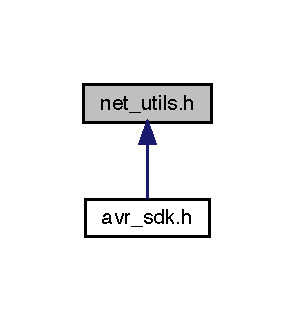
\includegraphics[width=142pt]{net__utils_8h__dep__incl}
\end{center}
\end{figure}
\subsection*{Macros}
\begin{DoxyCompactItemize}
\item 
\mbox{\Hypertarget{net__utils_8h_a7b6f5e01e3645597817cefda60ee53d1}\label{net__utils_8h_a7b6f5e01e3645597817cefda60ee53d1}} 
\#define \hyperlink{net__utils_8h_a7b6f5e01e3645597817cefda60ee53d1}{I\+P\+V4\+\_\+\+S\+T\+R\+\_\+\+M\+I\+N\+\_\+\+L\+EN}~7
\begin{DoxyCompactList}\small\item\em Ex\+: 0.\+0.\+0.\+0. \end{DoxyCompactList}\item 
\mbox{\Hypertarget{net__utils_8h_af4784545f0f0e098c3ac72fe8e6c7150}\label{net__utils_8h_af4784545f0f0e098c3ac72fe8e6c7150}} 
\#define \hyperlink{net__utils_8h_af4784545f0f0e098c3ac72fe8e6c7150}{I\+P\+V4\+\_\+\+S\+T\+R\+\_\+\+M\+A\+X\+\_\+\+L\+EN}~15
\begin{DoxyCompactList}\small\item\em Ex\+: 255.\+255.\+255.\+255. \end{DoxyCompactList}\item 
\mbox{\Hypertarget{net__utils_8h_addad4b01a9d0f943e588e780b5eb27e7}\label{net__utils_8h_addad4b01a9d0f943e588e780b5eb27e7}} 
\#define \hyperlink{net__utils_8h_addad4b01a9d0f943e588e780b5eb27e7}{I\+P\+V4\+\_\+\+N\+E\+T\+M\+A\+S\+K\+\_\+\+S\+T\+R\+\_\+\+M\+I\+N\+\_\+\+L\+EN}~9
\begin{DoxyCompactList}\small\item\em Ex\+: 0.\+0.\+0.\+0/0. \end{DoxyCompactList}\item 
\mbox{\Hypertarget{net__utils_8h_a8b1e7e2f4f87a0d67d046d99bd8e1b5d}\label{net__utils_8h_a8b1e7e2f4f87a0d67d046d99bd8e1b5d}} 
\#define \hyperlink{net__utils_8h_a8b1e7e2f4f87a0d67d046d99bd8e1b5d}{I\+P\+V4\+\_\+\+N\+E\+T\+M\+A\+S\+K\+\_\+\+S\+T\+R\+\_\+\+M\+A\+X\+\_\+\+L\+EN}~18
\begin{DoxyCompactList}\small\item\em Ex\+: 255.\+255.\+255.\+255/32. \end{DoxyCompactList}\item 
\mbox{\Hypertarget{net__utils_8h_a32e2533263ec1945df5b847da2c277bd}\label{net__utils_8h_a32e2533263ec1945df5b847da2c277bd}} 
\#define \hyperlink{net__utils_8h_a32e2533263ec1945df5b847da2c277bd}{N\+E\+T\+M\+A\+S\+K\+\_\+\+M\+I\+N\+\_\+\+L\+EN}~1
\begin{DoxyCompactList}\small\item\em Ex\+: 0.\+0.\+0.\+0/1. \end{DoxyCompactList}\item 
\mbox{\Hypertarget{net__utils_8h_aca9ea32f97406372853faf6b2ef123df}\label{net__utils_8h_aca9ea32f97406372853faf6b2ef123df}} 
\#define \hyperlink{net__utils_8h_aca9ea32f97406372853faf6b2ef123df}{N\+E\+T\+M\+A\+S\+K\+\_\+\+M\+A\+X\+\_\+\+L\+EN}~32
\begin{DoxyCompactList}\small\item\em Ex\+: 0.\+0.\+0.\+0/32. \end{DoxyCompactList}\item 
\mbox{\Hypertarget{net__utils_8h_a96b7f44fce9f4f191054fb9fe6db1988}\label{net__utils_8h_a96b7f44fce9f4f191054fb9fe6db1988}} 
\#define {\bfseries I\+P\+V4\+\_\+\+N\+\_\+\+O\+C\+T\+E\+C\+TS}~4
\end{DoxyCompactItemize}
\subsection*{Functions}
\begin{DoxyCompactItemize}
\item 
\hyperlink{unionipv4addr__t}{ipv4addr\+\_\+t} \hyperlink{net__utils_8h_a2d486ef540262620e61b9a33263d7e50}{\+\_\+\+\_\+inet\+\_\+ipv4\+\_\+get\+Broadcast\+Addr} (\hyperlink{unionipv4addr__t}{ipv4addr\+\_\+t} ip, \hyperlink{unionipv4addr__t}{ipv4addr\+\_\+t} netmask)
\begin{DoxyCompactList}\small\item\em Recovers broadcast address given an ip and netmask. \end{DoxyCompactList}\item 
\hyperlink{unionipv4addr__t}{ipv4addr\+\_\+t} \hyperlink{net__utils_8h_a89bce19ecd33bd9f997ca703d71ad4a7}{\+\_\+\+\_\+inet\+\_\+ipv4\+\_\+get\+Broadcast\+Addr} (const char $\ast$ip)
\begin{DoxyCompactList}\small\item\em Recovers broadcast address given an ip and netmask in format X\+X\+X.\+X\+X\+X.\+X\+X\+X.\+X\+XX/\+XX. \end{DoxyCompactList}\item 
\hyperlink{unionipv4addr__t}{ipv4addr\+\_\+t} \hyperlink{net__utils_8h_aa64426514e1f1bae885e327e797a1762}{\+\_\+\+\_\+inet\+\_\+ipv4\+\_\+get\+Network\+Addr} (\hyperlink{unionipv4addr__t}{ipv4addr\+\_\+t} ip, \hyperlink{unionipv4addr__t}{ipv4addr\+\_\+t} netmask)
\begin{DoxyCompactList}\small\item\em Recovers network address given an ip and netmask. \end{DoxyCompactList}\item 
\hyperlink{unionipv4addr__t}{ipv4addr\+\_\+t} \hyperlink{net__utils_8h_a68a4b28081cbc704c62e62e1adf07775}{\+\_\+\+\_\+inet\+\_\+ipv4\+\_\+get\+Network\+Addr} (const char $\ast$ip)
\begin{DoxyCompactList}\small\item\em Recovers network address given an ip and netmask in format X\+X\+X.\+X\+X\+X.\+X\+X\+X.\+X\+XX/\+XX. \end{DoxyCompactList}\item 
u32t \hyperlink{net__utils_8h_ac3d886dd18ae09307c25a32704ef6b7b}{\+\_\+\+\_\+inet\+\_\+ipv4\+\_\+get\+Subnet} (const char $\ast$ip)
\begin{DoxyCompactList}\small\item\em Recovers subnet address given an ip and netmask in format X\+X\+X.\+X\+X\+X.\+X\+X\+X.\+X\+XX/\+XX. \end{DoxyCompactList}\item 
u32t \hyperlink{net__utils_8h_a2b0fe4a8ea60b422522d37c650d28e8e}{\+\_\+\+\_\+inet\+\_\+ipv4\+\_\+itosubnet} (u8t netmask)
\begin{DoxyCompactList}\small\item\em Converts netmask in notation 1-\/32 to uint32\+\_\+t. \end{DoxyCompactList}\item 
u32t \hyperlink{net__utils_8h_a4463fdfe2a910abc9b392bf035ab4dd0}{\+\_\+\+\_\+inet\+\_\+ipv4\+\_\+get\+Wildcard} (const char $\ast$ip)
\begin{DoxyCompactList}\small\item\em Recovers wildcard address given an ip and netmask. \end{DoxyCompactList}\item 
u32t \hyperlink{net__utils_8h_acdedf596c106aca1b78d447b908fd939}{\+\_\+\+\_\+inet\+\_\+ipv4\+\_\+itowildcard} (u8t netmask)
\begin{DoxyCompactList}\small\item\em Converts netmask in notation 1-\/32 to wildcard. \end{DoxyCompactList}\item 
size\+\_\+t \hyperlink{net__utils_8h_a8925389179a3f838709725e67feae1df}{\+\_\+\+\_\+inet\+\_\+ipv4\+\_\+get\+Number\+Clients} (const char $\ast$ip)
\begin{DoxyCompactList}\small\item\em Get number of client in a network. \end{DoxyCompactList}\item 
void \hyperlink{net__utils_8h_a405eb1f3adb7e6e9e111116bf67f5b76}{\+\_\+\+\_\+inet\+\_\+ipv4\+\_\+netmask\+\_\+split} (u8t $\ast$dst, const char $\ast$ip)
\begin{DoxyCompactList}\small\item\em Converts ip and netmask in format X\+X\+X.\+X\+X\+X.\+X\+X\+X.\+X\+XX/\+XX. Fills dst array. \end{DoxyCompactList}\item 
u8t \hyperlink{net__utils_8h_a01c029b38eed8ea9df3c56bf61de5945}{\+\_\+\+\_\+inet\+\_\+ipv4\+\_\+netmask\+\_\+split} (const char $\ast$ip)
\begin{DoxyCompactList}\small\item\em Recovers netmask from ip and netmask string in format X\+X\+X.\+X\+X\+X.\+X\+X\+X.\+X\+XX/\+XX. \end{DoxyCompactList}\item 
bool \hyperlink{net__utils_8h_aaebdf1d1dd06f7285b0b741a2c59ea1d}{\+\_\+\+\_\+inet\+\_\+ipv4\+\_\+is\+Valid\+IP} (const char $\ast$ip)
\begin{DoxyCompactList}\small\item\em Checks if given ip and netmask string is valid in format X\+X\+X.\+X\+X\+X.\+X\+X\+X.\+X\+XX/\+XX. \end{DoxyCompactList}\item 
\hyperlink{unionipv4addr__t}{ipv4addr\+\_\+t} \hyperlink{net__utils_8h_a02ad2e599436916b9ef5f2e11a82c183}{\+\_\+\+\_\+inet\+\_\+ipv4\+\_\+aton} (const std\+::string \&ip)
\begin{DoxyCompactList}\small\item\em Converts A\+S\+C\+II to Network an ip address. \end{DoxyCompactList}\item 
\hyperlink{unionipv4addr__t}{ipv4addr\+\_\+t} \hyperlink{net__utils_8h_aec1328db0249fbe999df0914e956e99b}{\+\_\+\+\_\+inet\+\_\+ipv4\+\_\+aton} (char $\ast$ip)
\begin{DoxyCompactList}\small\item\em Converts A\+S\+C\+II to Network an ip address. \end{DoxyCompactList}\item 
void \hyperlink{net__utils_8h_a6b4f328429adb76ec55c9bc1c78d24f2}{\+\_\+\+\_\+inet\+\_\+ipv4\+\_\+ntoa} (char $\ast$dst, \hyperlink{unionipv4addr__t}{ipv4addr\+\_\+t} ip)
\begin{DoxyCompactList}\small\item\em Converts Netwok to A\+S\+C\+II an ip address. \end{DoxyCompactList}\item 
std\+::string \hyperlink{net__utils_8h_a35dbe374ad82d07d77cdbbed84b1313e}{\+\_\+\+\_\+inet\+\_\+ipv4\+\_\+ntoa} (\hyperlink{unionipv4addr__t}{ipv4addr\+\_\+t} ip)
\begin{DoxyCompactList}\small\item\em Converts Netwok to A\+S\+C\+II an ip address. \end{DoxyCompactList}\end{DoxyCompactItemize}


\subsection{Function Documentation}
\mbox{\Hypertarget{net__utils_8h_a02ad2e599436916b9ef5f2e11a82c183}\label{net__utils_8h_a02ad2e599436916b9ef5f2e11a82c183}} 
\index{net\+\_\+utils.\+h@{net\+\_\+utils.\+h}!\+\_\+\+\_\+inet\+\_\+ipv4\+\_\+aton@{\+\_\+\+\_\+inet\+\_\+ipv4\+\_\+aton}}
\index{\+\_\+\+\_\+inet\+\_\+ipv4\+\_\+aton@{\+\_\+\+\_\+inet\+\_\+ipv4\+\_\+aton}!net\+\_\+utils.\+h@{net\+\_\+utils.\+h}}
\subsubsection{\texorpdfstring{\+\_\+\+\_\+inet\+\_\+ipv4\+\_\+aton()}{\_\_inet\_ipv4\_aton()}\hspace{0.1cm}{\footnotesize\ttfamily [1/2]}}
{\footnotesize\ttfamily \hyperlink{unionipv4addr__t}{ipv4addr\+\_\+t} \+\_\+\+\_\+inet\+\_\+ipv4\+\_\+aton (\begin{DoxyParamCaption}\item[{const std\+::string \&}]{ip }\end{DoxyParamCaption})}



Converts A\+S\+C\+II to Network an ip address. 


\begin{DoxyParams}[1]{Parameters}
\mbox{\tt in}  & {\em ip} & without netmask in format X\+X\+X.\+X\+X\+X.\+X\+X\+X.\+X\+XX \\
\hline
\end{DoxyParams}
\begin{DoxyReturn}{Returns}

\end{DoxyReturn}
\mbox{\Hypertarget{net__utils_8h_aec1328db0249fbe999df0914e956e99b}\label{net__utils_8h_aec1328db0249fbe999df0914e956e99b}} 
\index{net\+\_\+utils.\+h@{net\+\_\+utils.\+h}!\+\_\+\+\_\+inet\+\_\+ipv4\+\_\+aton@{\+\_\+\+\_\+inet\+\_\+ipv4\+\_\+aton}}
\index{\+\_\+\+\_\+inet\+\_\+ipv4\+\_\+aton@{\+\_\+\+\_\+inet\+\_\+ipv4\+\_\+aton}!net\+\_\+utils.\+h@{net\+\_\+utils.\+h}}
\subsubsection{\texorpdfstring{\+\_\+\+\_\+inet\+\_\+ipv4\+\_\+aton()}{\_\_inet\_ipv4\_aton()}\hspace{0.1cm}{\footnotesize\ttfamily [2/2]}}
{\footnotesize\ttfamily \hyperlink{unionipv4addr__t}{ipv4addr\+\_\+t} \+\_\+\+\_\+inet\+\_\+ipv4\+\_\+aton (\begin{DoxyParamCaption}\item[{char $\ast$}]{ip }\end{DoxyParamCaption})}



Converts A\+S\+C\+II to Network an ip address. 


\begin{DoxyParams}[1]{Parameters}
\mbox{\tt in}  & {\em ip} & without netmask in format X\+X\+X.\+X\+X\+X.\+X\+X\+X.\+X\+XX \\
\hline
\end{DoxyParams}
\begin{DoxyReturn}{Returns}

\end{DoxyReturn}
\mbox{\Hypertarget{net__utils_8h_a2d486ef540262620e61b9a33263d7e50}\label{net__utils_8h_a2d486ef540262620e61b9a33263d7e50}} 
\index{net\+\_\+utils.\+h@{net\+\_\+utils.\+h}!\+\_\+\+\_\+inet\+\_\+ipv4\+\_\+get\+Broadcast\+Addr@{\+\_\+\+\_\+inet\+\_\+ipv4\+\_\+get\+Broadcast\+Addr}}
\index{\+\_\+\+\_\+inet\+\_\+ipv4\+\_\+get\+Broadcast\+Addr@{\+\_\+\+\_\+inet\+\_\+ipv4\+\_\+get\+Broadcast\+Addr}!net\+\_\+utils.\+h@{net\+\_\+utils.\+h}}
\subsubsection{\texorpdfstring{\+\_\+\+\_\+inet\+\_\+ipv4\+\_\+get\+Broadcast\+Addr()}{\_\_inet\_ipv4\_getBroadcastAddr()}\hspace{0.1cm}{\footnotesize\ttfamily [1/2]}}
{\footnotesize\ttfamily \hyperlink{unionipv4addr__t}{ipv4addr\+\_\+t} \+\_\+\+\_\+inet\+\_\+ipv4\+\_\+get\+Broadcast\+Addr (\begin{DoxyParamCaption}\item[{\hyperlink{unionipv4addr__t}{ipv4addr\+\_\+t}}]{ip,  }\item[{\hyperlink{unionipv4addr__t}{ipv4addr\+\_\+t}}]{netmask }\end{DoxyParamCaption})}



Recovers broadcast address given an ip and netmask. 


\begin{DoxyParams}[1]{Parameters}
\mbox{\tt in}  & {\em ip} & \\
\hline
\mbox{\tt in}  & {\em netmask} & \\
\hline
\end{DoxyParams}
\begin{DoxyReturn}{Returns}
Broadcast address 
\end{DoxyReturn}
\mbox{\Hypertarget{net__utils_8h_a89bce19ecd33bd9f997ca703d71ad4a7}\label{net__utils_8h_a89bce19ecd33bd9f997ca703d71ad4a7}} 
\index{net\+\_\+utils.\+h@{net\+\_\+utils.\+h}!\+\_\+\+\_\+inet\+\_\+ipv4\+\_\+get\+Broadcast\+Addr@{\+\_\+\+\_\+inet\+\_\+ipv4\+\_\+get\+Broadcast\+Addr}}
\index{\+\_\+\+\_\+inet\+\_\+ipv4\+\_\+get\+Broadcast\+Addr@{\+\_\+\+\_\+inet\+\_\+ipv4\+\_\+get\+Broadcast\+Addr}!net\+\_\+utils.\+h@{net\+\_\+utils.\+h}}
\subsubsection{\texorpdfstring{\+\_\+\+\_\+inet\+\_\+ipv4\+\_\+get\+Broadcast\+Addr()}{\_\_inet\_ipv4\_getBroadcastAddr()}\hspace{0.1cm}{\footnotesize\ttfamily [2/2]}}
{\footnotesize\ttfamily \hyperlink{unionipv4addr__t}{ipv4addr\+\_\+t} \+\_\+\+\_\+inet\+\_\+ipv4\+\_\+get\+Broadcast\+Addr (\begin{DoxyParamCaption}\item[{const char $\ast$}]{ip }\end{DoxyParamCaption})}



Recovers broadcast address given an ip and netmask in format X\+X\+X.\+X\+X\+X.\+X\+X\+X.\+X\+XX/\+XX. 


\begin{DoxyParams}[1]{Parameters}
\mbox{\tt in}  & {\em ip} & \\
\hline
\end{DoxyParams}
\begin{DoxyReturn}{Returns}
Broadcast address 
\end{DoxyReturn}
\mbox{\Hypertarget{net__utils_8h_aa64426514e1f1bae885e327e797a1762}\label{net__utils_8h_aa64426514e1f1bae885e327e797a1762}} 
\index{net\+\_\+utils.\+h@{net\+\_\+utils.\+h}!\+\_\+\+\_\+inet\+\_\+ipv4\+\_\+get\+Network\+Addr@{\+\_\+\+\_\+inet\+\_\+ipv4\+\_\+get\+Network\+Addr}}
\index{\+\_\+\+\_\+inet\+\_\+ipv4\+\_\+get\+Network\+Addr@{\+\_\+\+\_\+inet\+\_\+ipv4\+\_\+get\+Network\+Addr}!net\+\_\+utils.\+h@{net\+\_\+utils.\+h}}
\subsubsection{\texorpdfstring{\+\_\+\+\_\+inet\+\_\+ipv4\+\_\+get\+Network\+Addr()}{\_\_inet\_ipv4\_getNetworkAddr()}\hspace{0.1cm}{\footnotesize\ttfamily [1/2]}}
{\footnotesize\ttfamily \hyperlink{unionipv4addr__t}{ipv4addr\+\_\+t} \+\_\+\+\_\+inet\+\_\+ipv4\+\_\+get\+Network\+Addr (\begin{DoxyParamCaption}\item[{\hyperlink{unionipv4addr__t}{ipv4addr\+\_\+t}}]{ip,  }\item[{\hyperlink{unionipv4addr__t}{ipv4addr\+\_\+t}}]{netmask }\end{DoxyParamCaption})}



Recovers network address given an ip and netmask. 


\begin{DoxyParams}[1]{Parameters}
\mbox{\tt in}  & {\em ip} & \\
\hline
\mbox{\tt in}  & {\em netmask} & \\
\hline
\end{DoxyParams}
\begin{DoxyReturn}{Returns}
Network address 
\end{DoxyReturn}
\mbox{\Hypertarget{net__utils_8h_a68a4b28081cbc704c62e62e1adf07775}\label{net__utils_8h_a68a4b28081cbc704c62e62e1adf07775}} 
\index{net\+\_\+utils.\+h@{net\+\_\+utils.\+h}!\+\_\+\+\_\+inet\+\_\+ipv4\+\_\+get\+Network\+Addr@{\+\_\+\+\_\+inet\+\_\+ipv4\+\_\+get\+Network\+Addr}}
\index{\+\_\+\+\_\+inet\+\_\+ipv4\+\_\+get\+Network\+Addr@{\+\_\+\+\_\+inet\+\_\+ipv4\+\_\+get\+Network\+Addr}!net\+\_\+utils.\+h@{net\+\_\+utils.\+h}}
\subsubsection{\texorpdfstring{\+\_\+\+\_\+inet\+\_\+ipv4\+\_\+get\+Network\+Addr()}{\_\_inet\_ipv4\_getNetworkAddr()}\hspace{0.1cm}{\footnotesize\ttfamily [2/2]}}
{\footnotesize\ttfamily \hyperlink{unionipv4addr__t}{ipv4addr\+\_\+t} \+\_\+\+\_\+inet\+\_\+ipv4\+\_\+get\+Network\+Addr (\begin{DoxyParamCaption}\item[{const char $\ast$}]{ip }\end{DoxyParamCaption})}



Recovers network address given an ip and netmask in format X\+X\+X.\+X\+X\+X.\+X\+X\+X.\+X\+XX/\+XX. 


\begin{DoxyParams}[1]{Parameters}
\mbox{\tt in}  & {\em ip} & and netmask in format X\+X\+X.\+X\+X\+X.\+X\+X\+X.\+X\+XX/\+XX \\
\hline
\end{DoxyParams}
\begin{DoxyReturn}{Returns}
Network address 
\end{DoxyReturn}
\mbox{\Hypertarget{net__utils_8h_a8925389179a3f838709725e67feae1df}\label{net__utils_8h_a8925389179a3f838709725e67feae1df}} 
\index{net\+\_\+utils.\+h@{net\+\_\+utils.\+h}!\+\_\+\+\_\+inet\+\_\+ipv4\+\_\+get\+Number\+Clients@{\+\_\+\+\_\+inet\+\_\+ipv4\+\_\+get\+Number\+Clients}}
\index{\+\_\+\+\_\+inet\+\_\+ipv4\+\_\+get\+Number\+Clients@{\+\_\+\+\_\+inet\+\_\+ipv4\+\_\+get\+Number\+Clients}!net\+\_\+utils.\+h@{net\+\_\+utils.\+h}}
\subsubsection{\texorpdfstring{\+\_\+\+\_\+inet\+\_\+ipv4\+\_\+get\+Number\+Clients()}{\_\_inet\_ipv4\_getNumberClients()}}
{\footnotesize\ttfamily size\+\_\+t \+\_\+\+\_\+inet\+\_\+ipv4\+\_\+get\+Number\+Clients (\begin{DoxyParamCaption}\item[{const char $\ast$}]{ip }\end{DoxyParamCaption})}



Get number of client in a network. 


\begin{DoxyParams}[1]{Parameters}
\mbox{\tt in}  & {\em up} & and netmask string in format X\+X\+X.\+X\+X\+X.\+X\+X\+X.\+X\+XX/\+XX \\
\hline
\end{DoxyParams}
\begin{DoxyReturn}{Returns}
Number of clients 
\end{DoxyReturn}
\mbox{\Hypertarget{net__utils_8h_ac3d886dd18ae09307c25a32704ef6b7b}\label{net__utils_8h_ac3d886dd18ae09307c25a32704ef6b7b}} 
\index{net\+\_\+utils.\+h@{net\+\_\+utils.\+h}!\+\_\+\+\_\+inet\+\_\+ipv4\+\_\+get\+Subnet@{\+\_\+\+\_\+inet\+\_\+ipv4\+\_\+get\+Subnet}}
\index{\+\_\+\+\_\+inet\+\_\+ipv4\+\_\+get\+Subnet@{\+\_\+\+\_\+inet\+\_\+ipv4\+\_\+get\+Subnet}!net\+\_\+utils.\+h@{net\+\_\+utils.\+h}}
\subsubsection{\texorpdfstring{\+\_\+\+\_\+inet\+\_\+ipv4\+\_\+get\+Subnet()}{\_\_inet\_ipv4\_getSubnet()}}
{\footnotesize\ttfamily u32t \+\_\+\+\_\+inet\+\_\+ipv4\+\_\+get\+Subnet (\begin{DoxyParamCaption}\item[{const char $\ast$}]{ip }\end{DoxyParamCaption})\hspace{0.3cm}{\ttfamily [inline]}}



Recovers subnet address given an ip and netmask in format X\+X\+X.\+X\+X\+X.\+X\+X\+X.\+X\+XX/\+XX. 


\begin{DoxyParams}[1]{Parameters}
\mbox{\tt in}  & {\em ip} & and netmask in format X\+X\+X.\+X\+X\+X.\+X\+X\+X.\+X\+XX/\+XX \\
\hline
\end{DoxyParams}
\begin{DoxyReturn}{Returns}
Subnet address 
\end{DoxyReturn}
\mbox{\Hypertarget{net__utils_8h_a4463fdfe2a910abc9b392bf035ab4dd0}\label{net__utils_8h_a4463fdfe2a910abc9b392bf035ab4dd0}} 
\index{net\+\_\+utils.\+h@{net\+\_\+utils.\+h}!\+\_\+\+\_\+inet\+\_\+ipv4\+\_\+get\+Wildcard@{\+\_\+\+\_\+inet\+\_\+ipv4\+\_\+get\+Wildcard}}
\index{\+\_\+\+\_\+inet\+\_\+ipv4\+\_\+get\+Wildcard@{\+\_\+\+\_\+inet\+\_\+ipv4\+\_\+get\+Wildcard}!net\+\_\+utils.\+h@{net\+\_\+utils.\+h}}
\subsubsection{\texorpdfstring{\+\_\+\+\_\+inet\+\_\+ipv4\+\_\+get\+Wildcard()}{\_\_inet\_ipv4\_getWildcard()}}
{\footnotesize\ttfamily u32t \+\_\+\+\_\+inet\+\_\+ipv4\+\_\+get\+Wildcard (\begin{DoxyParamCaption}\item[{const char $\ast$}]{ip }\end{DoxyParamCaption})\hspace{0.3cm}{\ttfamily [inline]}}



Recovers wildcard address given an ip and netmask. 


\begin{DoxyParams}[1]{Parameters}
\mbox{\tt in}  & {\em ip} & and netmask in format X\+X\+X.\+X\+X\+X.\+X\+X\+X.\+X\+XX/\+XX \\
\hline
\end{DoxyParams}
\begin{DoxyReturn}{Returns}

\end{DoxyReturn}
\mbox{\Hypertarget{net__utils_8h_aaebdf1d1dd06f7285b0b741a2c59ea1d}\label{net__utils_8h_aaebdf1d1dd06f7285b0b741a2c59ea1d}} 
\index{net\+\_\+utils.\+h@{net\+\_\+utils.\+h}!\+\_\+\+\_\+inet\+\_\+ipv4\+\_\+is\+Valid\+IP@{\+\_\+\+\_\+inet\+\_\+ipv4\+\_\+is\+Valid\+IP}}
\index{\+\_\+\+\_\+inet\+\_\+ipv4\+\_\+is\+Valid\+IP@{\+\_\+\+\_\+inet\+\_\+ipv4\+\_\+is\+Valid\+IP}!net\+\_\+utils.\+h@{net\+\_\+utils.\+h}}
\subsubsection{\texorpdfstring{\+\_\+\+\_\+inet\+\_\+ipv4\+\_\+is\+Valid\+I\+P()}{\_\_inet\_ipv4\_isValidIP()}}
{\footnotesize\ttfamily bool \+\_\+\+\_\+inet\+\_\+ipv4\+\_\+is\+Valid\+IP (\begin{DoxyParamCaption}\item[{const char $\ast$}]{ip }\end{DoxyParamCaption})}



Checks if given ip and netmask string is valid in format X\+X\+X.\+X\+X\+X.\+X\+X\+X.\+X\+XX/\+XX. 


\begin{DoxyParams}[1]{Parameters}
\mbox{\tt in}  & {\em ip} & and netmask string is valid in format X\+X\+X.\+X\+X\+X.\+X\+X\+X.\+X\+XX/\+XX \\
\hline
\end{DoxyParams}
\begin{DoxyReturn}{Returns}
True if valid, false if not 
\end{DoxyReturn}
\mbox{\Hypertarget{net__utils_8h_a2b0fe4a8ea60b422522d37c650d28e8e}\label{net__utils_8h_a2b0fe4a8ea60b422522d37c650d28e8e}} 
\index{net\+\_\+utils.\+h@{net\+\_\+utils.\+h}!\+\_\+\+\_\+inet\+\_\+ipv4\+\_\+itosubnet@{\+\_\+\+\_\+inet\+\_\+ipv4\+\_\+itosubnet}}
\index{\+\_\+\+\_\+inet\+\_\+ipv4\+\_\+itosubnet@{\+\_\+\+\_\+inet\+\_\+ipv4\+\_\+itosubnet}!net\+\_\+utils.\+h@{net\+\_\+utils.\+h}}
\subsubsection{\texorpdfstring{\+\_\+\+\_\+inet\+\_\+ipv4\+\_\+itosubnet()}{\_\_inet\_ipv4\_itosubnet()}}
{\footnotesize\ttfamily u32t \+\_\+\+\_\+inet\+\_\+ipv4\+\_\+itosubnet (\begin{DoxyParamCaption}\item[{u8t}]{netmask }\end{DoxyParamCaption})\hspace{0.3cm}{\ttfamily [inline]}}



Converts netmask in notation 1-\/32 to uint32\+\_\+t. 


\begin{DoxyParams}[1]{Parameters}
\mbox{\tt in}  & {\em netmask} & \\
\hline
\end{DoxyParams}
\begin{DoxyReturn}{Returns}
Converted value 
\end{DoxyReturn}
\mbox{\Hypertarget{net__utils_8h_acdedf596c106aca1b78d447b908fd939}\label{net__utils_8h_acdedf596c106aca1b78d447b908fd939}} 
\index{net\+\_\+utils.\+h@{net\+\_\+utils.\+h}!\+\_\+\+\_\+inet\+\_\+ipv4\+\_\+itowildcard@{\+\_\+\+\_\+inet\+\_\+ipv4\+\_\+itowildcard}}
\index{\+\_\+\+\_\+inet\+\_\+ipv4\+\_\+itowildcard@{\+\_\+\+\_\+inet\+\_\+ipv4\+\_\+itowildcard}!net\+\_\+utils.\+h@{net\+\_\+utils.\+h}}
\subsubsection{\texorpdfstring{\+\_\+\+\_\+inet\+\_\+ipv4\+\_\+itowildcard()}{\_\_inet\_ipv4\_itowildcard()}}
{\footnotesize\ttfamily u32t \+\_\+\+\_\+inet\+\_\+ipv4\+\_\+itowildcard (\begin{DoxyParamCaption}\item[{u8t}]{netmask }\end{DoxyParamCaption})\hspace{0.3cm}{\ttfamily [inline]}}



Converts netmask in notation 1-\/32 to wildcard. 


\begin{DoxyParams}[1]{Parameters}
\mbox{\tt in}  & {\em netmask} & \\
\hline
\end{DoxyParams}
\begin{DoxyReturn}{Returns}
Wildcard 
\end{DoxyReturn}
\mbox{\Hypertarget{net__utils_8h_a405eb1f3adb7e6e9e111116bf67f5b76}\label{net__utils_8h_a405eb1f3adb7e6e9e111116bf67f5b76}} 
\index{net\+\_\+utils.\+h@{net\+\_\+utils.\+h}!\+\_\+\+\_\+inet\+\_\+ipv4\+\_\+netmask\+\_\+split@{\+\_\+\+\_\+inet\+\_\+ipv4\+\_\+netmask\+\_\+split}}
\index{\+\_\+\+\_\+inet\+\_\+ipv4\+\_\+netmask\+\_\+split@{\+\_\+\+\_\+inet\+\_\+ipv4\+\_\+netmask\+\_\+split}!net\+\_\+utils.\+h@{net\+\_\+utils.\+h}}
\subsubsection{\texorpdfstring{\+\_\+\+\_\+inet\+\_\+ipv4\+\_\+netmask\+\_\+split()}{\_\_inet\_ipv4\_netmask\_split()}\hspace{0.1cm}{\footnotesize\ttfamily [1/2]}}
{\footnotesize\ttfamily void \+\_\+\+\_\+inet\+\_\+ipv4\+\_\+netmask\+\_\+split (\begin{DoxyParamCaption}\item[{u8t $\ast$}]{dst,  }\item[{const char $\ast$}]{ip }\end{DoxyParamCaption})}



Converts ip and netmask in format X\+X\+X.\+X\+X\+X.\+X\+X\+X.\+X\+XX/\+XX. Fills dst array. 


\begin{DoxyParams}[1]{Parameters}
\mbox{\tt out}  & {\em dst} & The array where is stored the conversion \mbox{[}octect0, octect1, octect2, octect3, netmask\mbox{]} \\
\hline
\mbox{\tt in}  & {\em ip} & The IP string in format X\+X\+X.\+X\+X\+X.\+X\+X\+X.\+X\+XX/\+XX \\
\hline
\end{DoxyParams}
\mbox{\Hypertarget{net__utils_8h_a01c029b38eed8ea9df3c56bf61de5945}\label{net__utils_8h_a01c029b38eed8ea9df3c56bf61de5945}} 
\index{net\+\_\+utils.\+h@{net\+\_\+utils.\+h}!\+\_\+\+\_\+inet\+\_\+ipv4\+\_\+netmask\+\_\+split@{\+\_\+\+\_\+inet\+\_\+ipv4\+\_\+netmask\+\_\+split}}
\index{\+\_\+\+\_\+inet\+\_\+ipv4\+\_\+netmask\+\_\+split@{\+\_\+\+\_\+inet\+\_\+ipv4\+\_\+netmask\+\_\+split}!net\+\_\+utils.\+h@{net\+\_\+utils.\+h}}
\subsubsection{\texorpdfstring{\+\_\+\+\_\+inet\+\_\+ipv4\+\_\+netmask\+\_\+split()}{\_\_inet\_ipv4\_netmask\_split()}\hspace{0.1cm}{\footnotesize\ttfamily [2/2]}}
{\footnotesize\ttfamily u8t \+\_\+\+\_\+inet\+\_\+ipv4\+\_\+netmask\+\_\+split (\begin{DoxyParamCaption}\item[{const char $\ast$}]{ip }\end{DoxyParamCaption})}



Recovers netmask from ip and netmask string in format X\+X\+X.\+X\+X\+X.\+X\+X\+X.\+X\+XX/\+XX. 


\begin{DoxyParams}[1]{Parameters}
\mbox{\tt in}  & {\em ip} & \\
\hline
\end{DoxyParams}
\begin{DoxyReturn}{Returns}
Netmask in range 1 -\/ 32 
\end{DoxyReturn}
\mbox{\Hypertarget{net__utils_8h_a6b4f328429adb76ec55c9bc1c78d24f2}\label{net__utils_8h_a6b4f328429adb76ec55c9bc1c78d24f2}} 
\index{net\+\_\+utils.\+h@{net\+\_\+utils.\+h}!\+\_\+\+\_\+inet\+\_\+ipv4\+\_\+ntoa@{\+\_\+\+\_\+inet\+\_\+ipv4\+\_\+ntoa}}
\index{\+\_\+\+\_\+inet\+\_\+ipv4\+\_\+ntoa@{\+\_\+\+\_\+inet\+\_\+ipv4\+\_\+ntoa}!net\+\_\+utils.\+h@{net\+\_\+utils.\+h}}
\subsubsection{\texorpdfstring{\+\_\+\+\_\+inet\+\_\+ipv4\+\_\+ntoa()}{\_\_inet\_ipv4\_ntoa()}\hspace{0.1cm}{\footnotesize\ttfamily [1/2]}}
{\footnotesize\ttfamily void \+\_\+\+\_\+inet\+\_\+ipv4\+\_\+ntoa (\begin{DoxyParamCaption}\item[{char $\ast$}]{dst,  }\item[{\hyperlink{unionipv4addr__t}{ipv4addr\+\_\+t}}]{ip }\end{DoxyParamCaption})}



Converts Netwok to A\+S\+C\+II an ip address. 


\begin{DoxyParams}[1]{Parameters}
\mbox{\tt out}  & {\em dst} & The resulting string \\
\hline
\mbox{\tt in}  & {\em ip} & without netmask in format X\+X\+X.\+X\+X\+X.\+X\+X\+X.\+X\+XX \\
\hline
\end{DoxyParams}
\mbox{\Hypertarget{net__utils_8h_a35dbe374ad82d07d77cdbbed84b1313e}\label{net__utils_8h_a35dbe374ad82d07d77cdbbed84b1313e}} 
\index{net\+\_\+utils.\+h@{net\+\_\+utils.\+h}!\+\_\+\+\_\+inet\+\_\+ipv4\+\_\+ntoa@{\+\_\+\+\_\+inet\+\_\+ipv4\+\_\+ntoa}}
\index{\+\_\+\+\_\+inet\+\_\+ipv4\+\_\+ntoa@{\+\_\+\+\_\+inet\+\_\+ipv4\+\_\+ntoa}!net\+\_\+utils.\+h@{net\+\_\+utils.\+h}}
\subsubsection{\texorpdfstring{\+\_\+\+\_\+inet\+\_\+ipv4\+\_\+ntoa()}{\_\_inet\_ipv4\_ntoa()}\hspace{0.1cm}{\footnotesize\ttfamily [2/2]}}
{\footnotesize\ttfamily std\+::string \+\_\+\+\_\+inet\+\_\+ipv4\+\_\+ntoa (\begin{DoxyParamCaption}\item[{\hyperlink{unionipv4addr__t}{ipv4addr\+\_\+t}}]{ip }\end{DoxyParamCaption})}



Converts Netwok to A\+S\+C\+II an ip address. 


\begin{DoxyParams}[1]{Parameters}
\mbox{\tt in}  & {\em ip} & without netmask in format X\+X\+X.\+X\+X\+X.\+X\+X\+X.\+X\+XX \\
\hline
\end{DoxyParams}
\begin{DoxyReturn}{Returns}
Ther resulting string 
\end{DoxyReturn}

%--- End generated contents ---

% Index
\backmatter
\newpage
\phantomsection
\clearemptydoublepage
\addcontentsline{toc}{chapter}{Index}
\printindex

\end{document}
